%%%%%%%%%%%%%%%%%%%%%%%%%%%%%%%%%%%%%%%%%%%%%%%%%%%%%%%%%%%%%%%%%%%%%%%%%%%%%%%%%%%%%%%%%%%
%%
%% The updated version of this document should be downloaded from
%%      https://github.com/jp-um/university_of_malta_LaTeX_dissertation_template
%%
%% In case of any difficulties please contact Dr JP Ebejer on jean.p.ebejer@um.edu.mt
%%
%%%%%%%%%%%%%%%%%%%%%%%%%%%%%%%%%%%%%%%%%%%%%%%%%%%%%%%%%%%%%%%%%%%%%%%%%%%%%%%%%%%%%%%%%%%

%% Before you embark on this quest you should probably read some of:
%% Deadly sins - http://mirrors.ctan.org/info/l2tabu/english/l2tabuen.pdf
%% Writing a thesis in LaTeX - http://tug.org/pracjourn/2008-1/mori/mori.pdf

\RequirePackage[l2tabu, orthodox]{nag} % tells you of any bad LaTeX usage
% must be first thing in class (with the exception of comments)

%% There is one option you should define; oneside or twoside
%% Use twoside for your viva docs (examiners hate long docs they need to carry around)
%% and oneside for the final thing you submit to the library.  Note that margins will
%% change accordingly

%\documentclass[twosie]{um}  % custom University of Malta project/dissertation/thesis
\documentclass[]{um}  % custom University of Malta project/dissertation/thesis


%% **************** (Your) Packages (Start) ******************

% \listfiles % uncomment this to know which packages you are using
% the list of packages will be in the bottom of the .log file

%% Note that packges may already be loaded from the um (and memoir) classes.
%% Do not add your packages to the template, but rather add them here.

\usepackage{blindtext} %% for some dummy text, remove in your writeup
\usepackage{coffee4}    %% for some fun
\usepackage{amsmath} %% line breaks equation
\usepackage{float}
\usepackage{multirow} %% for multirow tables
\usepackage{pgfplotstable,filecontents} %% for tables
\usepackage{pgfplots} %% for plots
%\usepackage{tikz} %% for plots
\usepackage{cancel} %% Cancel test
\usepackage{tabularx} %% for tables
\usepackage{booktabs}
\usepackage{makecell}
\usepackage{siunitx}
\usepackage{tcolorbox}
\usepackage{ulem} % to cancel / strikeout text
\usepackage{arydshln} % hdashlines
\usepackage{tabu}% http://ctan.org/pkg/tabu
\usepackage{subcaption}
\usepackage{textcomp}

% Captions for queations
\DeclareCaptionType{equ}[][]


\setlength\intextsep{18pt} % space between figures

\setlength\dashlinedash{0.5pt}
\setlength\dashlinegap{2pt}
\setlength\arrayrulewidth{0.5pt}

%% ***************** (Your) Packages (End) *******************


%% **************** (Your) Data (Start) ******************

\title{Predicting Spring Back in Sheet Metal Forming }
% use \\ here otherwise you get a justified title
% note capitalization of the title (only common
% words in lower case)
\tagline{A Comparative Study of Machine Learning Models and Evaluation of
Interpretability for Enhanced Process Insights}
\author{Philipp Kurrle}            % your full name
\authorID{123456}                   % your University Identifier
\supervisor{Prof. Dr. Ulrike Pado}              % your supervisor(s) name - no . in Dr
\cosupervisor{M. Sc. Peter Lange}                % your cosupervisor(s) name - no . in Dr *OPTIONAL*
\university{Hochschule für Technik}

% simply comment out the above line if absent
\department{Faculty of Measurement, Computer Science and Mathematics}   % your department (e.g. Artificial Intelligence)
\faculty{Master’s Programme in Software Technology}
\degreeName{M.Sc. in Software Technology}       % the degree you are reading
% note the \ after the dot, so not to consider it a fullstop
\doctype{thesis}               % the type of document (fyp, dissertation, thesis)
\degreeDate{\monthyeardate\today}    % when did you submit (officially after your corrections)
%%\subjectcode{ICS5200}                % the study unit-code (currently not used)

%% ***************** (Your) Data (End) *******************

%%
\renewcommand{\chapterheadstart}{\vspace*{\beforechapskip}}
\setlength\beforechapskip{0mm}


%% ******** (Your) Document Settings (Start) *************

% You should have an images directory in every chapX subdir
% NOTE:  Trailing / for subdirs is required.
\graphicspath{{./images/}{./chap1/images/}{./chap2/images/}{./chap3/images/}{./chap4/images/}
        {./chap5/images/}{./appA/images/}}

\makeindex

%% ********* (Your) Document Settings (End) **************

% DOCTOR'S (JP) ORDERS: MAKE SURE TO READ MY TWO BLOG ENTRIES WITH
% CONTENT AND LaTeX TIPS FOR YOUR WRITE-UP.  THESE ARE BASED ON  
% EXAMINER'S FEEDBACK
%
% URLS:
% https://bitsilla.com/blog/2019/03/content-tips-for-your-dissertation-or-project-write-up/
% https://bitsilla.com/blog/2019/01/latex-tips-for-your-dissertation-or-project-write-up/

% end the preamble and start the document

\begin{document}

    % Do not indent paragraphs
    \setlength{\parindent}{0pt}
    \parskip = 8pt

    \frontmatter
    \maketitle
    %\begin{copyrightenv}
\end{copyrightenv}


    %\begin{acknowledgements}
These are the acknowledgements. \blindtext
\end{acknowledgements}   % include an acknowledgements.tex file
    %% For tips on how to write a great abstract, have a look at
%%	-	https://www.cdc.gov/stdconference/2018/How-to-Write-an-Abstract_v4.pdf (presentation, start here)
%%	-	https://users.ece.cmu.edu/~koopman/essays/abstract.html
%%	-	https://search.proquest.com/docview/1417403858
%%  - 	https://www.sciencedirect.com/science/article/pii/S037837821830402X

%\begin{abstract}
\section*{Abstract}
\noindent Sheet metal bending is a widely ued manufacturing process in various industries such as automotive,
aerospace and construction.
One of the challenges in this process is the accurate prediction and compensation of spring back, which occurs
due the elastic recovery of the material after bending.
Inaccurate predictions of spring back can lead do fitting issues, increased costs and reduced product quality.
This study aims to research the potential of Machine Learning (ML) models to predict the spring back in sheet
metal bending using real-world air-bending data.

Three hypotheses were formulated and tested in this study.
First, it was hypothesized that ML models can accurately predict spring back, outperforming traditional trial-and-error methods.
Second, it was hypothesised that specific ML models or combinations of models would yield better performance
based on six Design Principles.
Third, it was hypothesized that ML models with high interpretability can provide valuable insights into the
factors contributing to spring back.

The results of this study support all three hypotheses, demonstrating the effectiveness of ML models in predicting the
spring back in sheet metal bending.
The Multi-Layer-Perceptron and Support Vector Machine models achieved the best performance with a root mean squared
error (RMSE) of 0.2 mm. Multiple models statisfy the highest accuracy level of the ISO 2768.
Additionally non-linear interactions between the different features in the dataset where found and analysed within
the dataset.
The findings also highlight the importance of selecting suitable ML models for specific applications.


In conclusion, this study demonstrates the potential of ML models to accurately predict and compensate for spring
back in sheet metal forming processes, leading to improved product quality and reduced manufacturing costs.
The findings have implications for both the understanding of spring back phenomena and the development of more
effective compensation strategies in the sheet metal forming industry.
%\end{abstract}\if@openright\cleardoublepage\else\clearpage\fi
    \tableofcontents*\if@openright\cleardoublepage\else\clearpage\fi
    \listoffigures*\if@openright\cleardoublepage\else\clearpage\fi
    \listoftables*\if@openright\cleardoublepage\else\clearpage\fi
    %% will only print what is used ... useful.
%% also acronyms are clickable, which is awesome

\chapter{List of Abbreviations} %% \chapter*{List of Abbreviations} not to appear in LoC
\markboth{List of Abbreviations}{List of Abbreviations}
               
\begin{acronym}\itemsep-20pt\parsep-20pt %% if you remove these spacing params this list becomes huge!
\acro{CDMA}{Code Division Multiple Access}
\acro{GSM}{Global System for Mobile communication}
\acro{NAD+}[NAD\textsuperscript{+}]{Nicotinamide Adenine Dinucleotide}
\acro{NUA}{Not Used Acronym}
\acro{TDMA}{Time Division Multiple Access}
\acro{UA}{Used Acronym}
\acro{lox}[\ensuremath{LOX}]{Liquid Oxygen}
\acro{lh2}[\ensuremath{LH_2}]{Liquid Hydrogen}
\acro{IC}{Integrated Circuit}
\acro{BUT}{Block Under Test}
\acrodefplural{BUT}{Blocks Under Test}    
\acro{ML}{Machine Learning}
\acro{SVM}{Support Vector Machine}
\acro{SVR}{Support Vector Regression}
\acro{ANN}{Artificial Neural Network}
\acro{FEM}{Finite Element Method}
\acro{DSR}{Design Science Research}
\acro{DP}{Design Principles}
\acro{GQM}{Goal-Question-Metric}
\acro{RF}{Random forest}
\acro{RFR}{Random Forest Regression}
\acro{DT}{Decision tree}
\acro{RMSE}{Root Mean Squared Error}
\acro{MSE}{mean squared error}
\acro{MAE}{Mean Absolute Error}
\acro{LOOCV}{Leave-one-out Cross Validation}
\acro{CV}{Cross-validation}
\acro{ELA}{Equalized Loss of Accuracy}
\acro{MLA}{Mean Loss of Accuracy}
\acro{BIC}{Bayesian Information Criterion}
\acro{LPOCV}{Leave-P-Out-Cross-Validation}
\acro{LR}{Linear Regression}
\acro{DT}{Decision Tree}
\acro{ET}{Extra Trees}
\acro{MLP}{Multi-layer Perceptron}
\acro{GBT}{Gradient boosted trees}
\acro{FDP}{Feature Dependences Plots}
\acro{PDP}{Partial Dependence Plots}
\end{acronym}
\if@openright\cleardoublepage\else\clearpage\fi

%% Note: always use \input as you cannot nest \includes (amongst other things)
    \pagestyle{umpage}
    \floatpagestyle{umpage}
    \mainmatter
    \chapter{Introduction}

Sheet metal forming has been used for centuries in different manufacturing industries to create a wide range of products for different applications. 
Sheet metal bending and stamping can be considered as the most important variants in the forming industry. \cite[p. 1]{cruz_applicationmachinelearning_2021} 
Therefore these have been continuously improved in recent decades to meet the growing demand especially in  automotive and aircraft industries with the goal to reduce energy efficiency and emissions. \cite[p. 4]{zheng_reviewformingtechniques_2018}

Sprinback is a common phenomenon in sheet metal forming processes. It is a deformation of the sheet metal that occurs when the sheet metal is bent. Therefore, predicting the spring back is important to reduce the number of trial and error cycles in the manufacturing process. \cite[p. 1]{cruz_applicationmachinelearning_2021} 
Sheet metal forming is a complex process that involves a large number of variables and parameters Therefore, it is difficult to predict the spring back accurately, which makes it an interesting case for machine learning.

In order to predict springback with minimium errors, this thesis build and evaluates different machine learning models to predict the springback of a sheet metal. The models are evaluated based on the mean absolute error (MAE) and the root mean squared error (RMSE). The best model is then used to predict the springback of a sheet metal with different parameters. 

% Sheet metal forming is a manufacturing process that is
% commonly used for producing high-volume and low-cost
% components in the automotive, aircraft and home appliance
% industries. In this process, forces are applied to the metallic
% sheet to modify its geometry, enabling the production of
% complex shapes. The forces are applied by tools whose
% geometry dictates the shape of the component. The process
% design is complex because only the final shape of the
% component is known. Moreover, the process is highly
% nonlinear due to the large deformations imposed to the
% metal sheet, which presents plastic behaviour, but also as a
% result of the evolutionary boundary conditions imposed by
% the contact between the tools and the sheet. The conven-
% tional process design is based on empirical knowledge and
% an experimental ‘‘trial-and-error’’ approach. In 
% \cite[]{dib_singleensembleclassifiers_2020}
    \chapter{Theoretical Foundations}\label{ch:theoretical-foundations}


\section{Sheet Metal}\label{sec:sheet-metal}
% Definition
Sheet metal is typically produced through the process of flat rolling various types of metals, resulting in a
characteristic aspect ratio of surface area thickness that typically falls within the range of
0.4\,mm to 6\,mm.
When the value exceeds this particular range, it is classified as a ``plate'', whereas if it falls below the range,
it is classified as a ``foil''
~\cite[p. 405]{groover_fundamentalsmodernmanufacturing_2020}.
% Material
Due to its accessibility, good formability, and sufficient strength for the majority of uses, low-carbon steel is a
regularly used type of sheet metal
~\cite[p. 405]{groover_fundamentalsmodernmanufacturing_2020}.
% Commercial importance
Sheet metals play a vital role in many industries for example automotive and aerospace to reduce the weight of
products~\cite[p. 1]{zheng_reviewformingtechniques_2018}.

\subsection{Sheet Metal Manufacturing}\label{subsec:sheet-metal-manufacturing}
% Manufacturing methods
The process of working with sheet metal is known as sheet-metal press-working and is often done with machine tools
called presses.
Utilizing so called ``punch-and-die tooling'' that is specifically made for these procedures, stamping presses are
employed to complete these processes
~\cite[p. 405]{groover_fundamentalsmodernmanufacturing_2020}.
The punch is a shaped tool that is usually mounted as upper part on the press ram and applies
pressure on the sheet metal to shape it.
The die is a stationary tool that is mounted in the press bed and provides a support surface for
the sheet metal and also defines the shape of the finished
product~\cref{sec:bending}~\cite[p. 412]{groover_fundamentalsmodernmanufacturing_2020}.
\cref{fig:bending-methods} shows the tooling setup together with a sheet metal being bend.
While the term `punch' is quite intuitive, the term ``die'' can cause confusion.
The term `die' is a typically term in metal working to refer to the lower or stationary part of a tooling setup.

Cutting, bending, and drawing are the three main groups of sheet metal forming processes.
While bending and drawing processes are used to mold sheet metal into the desired forms necessary for making certain
parts, cutting is used to separate huge sheets of material into smaller pieces.
~\cite[p. 405]{groover_fundamentalsmodernmanufacturing_2020}.
Drawing involves stretching the metal to create a convex or concave shape
~\cite[p. 416]{groover_fundamentalsmodernmanufacturing_2020}, while bending is ``defined as the straining of the
metal around a straight axis''
~\cite[p. 412]{groover_fundamentalsmodernmanufacturing_2020}.
This study focuses on metal bending and the bending method used in this study (Air Bending) deploys a mixture of
bending and drawing and will be explained in more detail in the next
section~\cite[pp. 416]{groover_fundamentalsmodernmanufacturing_2020}.


\section{Sheet Metal Bending}\label{sec:bending}
% Bending definition and description
Bending is a forming operation that is used to change the shape of a sheet metal by
applying a load to it.
It involves using force to shape the sheet metal into a desired form
~\cite[p. 1]{dib_singleensembleclassifiers_2020}.
The metal is subjected to a load that is greater than its yield strength but less than its ultimate tensile strength
, allowing the metal to be permanently deformed into a different shape.
~\cite[p. 1]{baig_machinelearningprediction_2021}.
% TODO Selbst hergeleitet aber keine Quelle?
This means that a load below the yield strength will not deform the metal, while a load above the utlimate tensile
strength will cause the metal to break.

Sheet metal bending is usually used to produce large quantities of components at low cost in various
industries~\cite[p. 1]{dib_singleensembleclassifiers_2020}.
The metal sheet experiences plastic deformation during the bending process, when the outside fibers are stretched and
the inside fibers are compressed.
As a result, the sheet metal curves in the direction of the applied load.
~\cite[pp. 1--3]{baig_machinelearningprediction_2021}.
The differently loaded cross-sectional areas are separated by a neutral plane in which theoretically no load occurs.
%The bending process creates a neutral plane, which an imaginary surface within the metal sheet where there is
%neither compression nor stretching.
If only the loaded cross-section is considered for simplification, the neutral plane is also referred to as the
neutral axis or neutral line
~\cite[pp. 67]{gustafson1998analytical}.
%It is also called neutral axis or neutral line~\cite[pp. 67]{gustafson1998analytical}.
\cref{fig:neutral-plane} shows the neutral plane after the bending operation, it is
visible, that it is closer to the inside of the bend than to the outside of the bend.
The arrows show where the metal was stretched and where it was compressed.

\begin{figure}[h]
    \begin{tcolorbox}[arc=0pt,boxrule=0.5pt, colback=white]
        \centering
        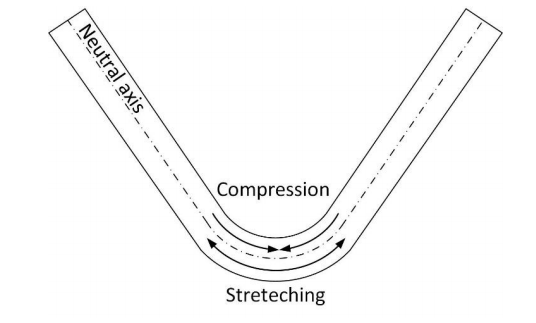
\includegraphics[width=0.6\textwidth]{chap2/images/neutral-plane}
    \end{tcolorbox}
    \caption{Neutral plane and the compression and stretching of a sheet metal
    ~\cite[p. 3]{baig_machinelearningprediction_2021}}
    \label{fig:neutral-plane}
\end{figure}

% TODO How curvature is achieved (keine Quelle?)
The amount of curvature that is achieved in the bending process is determined by the
amount of load applied, the thickness and properties of the metal and the location and length of the neutral plane.
By controlling these factors, it is possible to achieve precise and consistent results in the bending of sheet metal.

\subsection{Air Bending}\label{subsec:air-bending}
In the manufacturing industry, bending sheet metal is a critical process, allowing for the creation of various metal
shapes and configurations.
As can be seen in Groover (2020) V-bending and its variant, Air Bending, are both techniques that utilize punch-and
-die tooling ~\cite[p. 416]{groover_fundamentalsmodernmanufacturing_2020}.
The V-bending process, as shown in Figure~\ref{fig:v-bending}, entails pressing the metal into the shape of the die
to form precise and complex bends.
The die can take various shapes, including U-shaped, Z-shaped, or any other shape required to achieve the desired bend.

In contrast, air bending, as depicted in Figure~\ref{fig:air-bending}, utilizes an open die that only supports the
metal on each side.
This process permits a more extensive range of bend angles since the punch travel distance is not
restricted by the die.
Air bending can also achieve a tighter bend radius compared to V-bending, but it may result in
a slightly rounded bend.

\begin{figure}[h]
    \begin{tcolorbox}[arc=0pt,boxrule=0.5pt, colback=white]
        \centering
        \begin{subfigure}{0.4\textwidth}
            \centering
            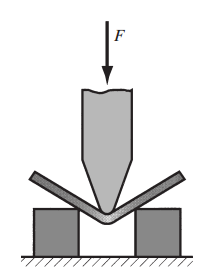
\includegraphics[width=\textwidth]{chap3/images/air-bending}
            \caption{Air bending}
            \label{fig:air-bending}
        \end{subfigure}
        \hfill
        \begin{subfigure}{0.4\textwidth}
            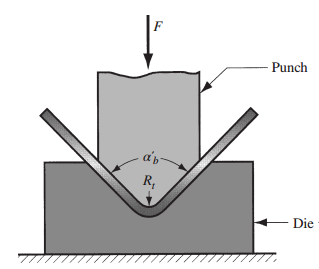
\includegraphics[width=\textwidth]{chap3/images/v-bending}
            \caption{V-Bending}
            \label{fig:v-bending}
        \end{subfigure}
        \hfill
    \end{tcolorbox}
    \caption{Differnt bending methods~\cite[pp. 416]{groover_fundamentalsmodernmanufacturing_2020}}
    \label{fig:bending-methods}
\end{figure}

% Usage of air bending
In the automotive sector, air bending is frequently utilized to create sheet metal components
~\cite[p. 342]{kim_predictionbendallowance_2007}.
Because it is flexible, it can achieve a variety of bending angles with the same punch-and-die tooling, it
is usually the most popular bending technique
~\cite[p. 3]{miranda_formingspringbackprediction_2018}~\cite[p. 1]{cruz_applicationmachinelearning_2021}.

Modern press machines are frequently fitted with "computer numerical control" (CNC) systems, which automatically
regulate the bending process and generate the desired shape.
~\cite[p. 3]{miranda_formingspringbackprediction_2018}
The process parameters are explained in \cref{fig:process_parameters}.

\subsubsection{Spring Back}\label{subsubsec:spring-back}
% How the spring back is created
After the deformation pressure is released, there is still
some elastic energy remaining in the bent part.
As a result, the bent part will partially return to its original
shape, which is known as spring back
~\cite[p. 413--414]{groover_fundamentalsmodernmanufacturing_2020}.

\cref{fig:spring-back} shows the spring back of a metal plate after the punch was removed.
The spring back is determined by the angle of the bent part after the punch is removed compared to the angle when
the punch was still applied.
The solid line shows the metal plate in its original form when the punch was still
applied.
The dashed line shows the metal plate after the punch was removed.

\begin{figure}[h]
    \centering
    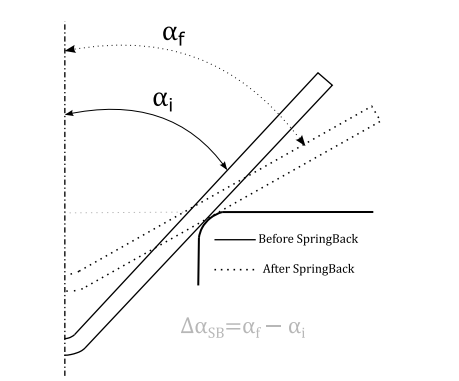
\includegraphics[width=0.5\textwidth]{chap3/images/spring-back}
    \caption{Spring back~\cite[p. 5]{cruz_applicationmachinelearning_2021}}
    \label{fig:spring-back}
\end{figure}

The angle before the spring back is usually denoted as $\alpha_i$ and the angle after spring back as $\alpha_f$.
% Introduce of formula
The spring back ($\Delta \alpha_{SB}$) is therefore the difference between $\alpha_f$ and
$\alpha_i$ as show in equation~\ref*{eq:calculation_springback}~\cite[p. 6]{cruz_applicationmachinelearning_2021}.


\begin{tcolorbox}[arc=0pt,boxrule=0.5pt]
    \begin{equation}
        \delta \alpha_{SB} = \alpha_f - \alpha_i
        \label{eq:calculation_springback}
    \end{equation}
\end{tcolorbox}

To tackle this problem, there are various techniques to compensate for spring back.
One commonly used approach is over bending, wherein the punch angle and radius are fabricated smaller than the
specified angle.
Prerequisite for all compensation methods is that the amount of spring back is known therefore
the accurate prediction of the spring back play an important role in the manufacturing
process ~\cite[p. 114]{groover_fundamentalsmodernmanufacturing_2020}.


\section{Machine Learning}\label{sec:machine-learning}
\cite{muller_introductionmachinelearning_2016} describe machine learning as ``Machine learning is about extracting
knowledge from data.'' and ``it is a research field at the intersection of statistics, artificial intelligence, and
computer science and is also known as predictive analytics or statistical learning.''
~\cite[p. 1]{muller_introductionmachinelearning_2016}.

The purpose of the model is to make predictions or decisions without explicitly requiring programming to do so.
\cite{el2015machine} use programming terms to explain thad ML models rather than being ``hard coded'', are ``soft
coded'', which means that they naturally alter their structure through repetition to increase their performance in
performing the target task ~\cite[pp. 4]{el2015machine}~\cite[pp. 151--170]{koza1996automated}.
``This adaptive process is known as training, and it involves providing the algorithm with input data samples and the
expected outputs, allowing the system to optimize itself to achieve the desired result not only with the training
inputs but also with new, previously unseen data.''
~\cite[pp. 4]{el2015machine}.
The training is the fundamental aspect of \ac{ML} and it can be continuous allowing the algorithm to
learn from new data and its mistakes~\cite[pp. 4]{el2015machine}.

Machine learning algorithms have numerous applications in fields just as example
agriculture (\cite{yoosefzadeh2021application}), computer vision (\cite{hu2020voronoi}) or metal working
(see section~\ref{sec:state-of-research}).

\subsection{Terminology}\label{subsec:terminology}
This study tries to use common terminology for \ac{ML} to make it easier to understand:
To carry out machine learning, a \textit{dataset} (~\cite[p. 3]{zhou_machinelearning_2021}) is required as the
initial foundation.
A dataset is composed of \textit{samples}, with each sample being a single row or observation.
For example, if a dataset contains information about metal sheet bending, each row would represent a single bend.

A \textit{feature} is an individual measurable property or characteristic of the data, and the associated value is
called an \textit{attribute}.
A feature could be, for example, the thickness of a sheet metal component, and the attribute could be 3 mm.
Features used to predict the outcome of a sample are called \textit{independent features} or \textit{input}, while the
outcome feature is referred to as the \textit{dependent feature} or \textit{target}.
In this study, the spring back is the dependent feature, while the other features which will be explained later are
independent features.
The dataset of this study will be explained in~\cref{subsec:dataset-exploration}.

The process of using machine learning algorithms to create a model is called \textit{training} or \textit{fitting}
~\cite[p. 4]{el2015machine}, and the data used for that process is commonly referred to as \textit{training data}.
Usually, the training data is a subset of the whole dataset.
The process of using the model to make predictions on new, unseen data is called
\textit{generalization}
~\cite[pp. 26--27]{muller_introductionmachinelearning_2016}~\cite[p. 4]{zhou_machinelearning_2021}.
The test-train split is described in more detail in section~\ref{subsec:training-test-split}.

The outcome of the learning process is referred to as a \textit{model} that can be used to make predictions on new,
unseen data.\ac{ML} algorithms are also often referred as \textit{learners}.

\subsection{Supervised Learning and Unsupervised Learning}\label{subsec:supervised-learning}
Learning tasks are classified into two types based on whether or not the outcome is already included in the training
data.
There are two types of learning: supervised learning and unsupervised learning.
~\cite[p. 4]{zhou_machinelearning_2021}.

Supervised learning is employed when not only the independent features but also the dependent feature is known.
Since this is the case in the dataset used in this study, supervised learning is the preferred
method
~\cite[p. 2]{muller_introductionmachinelearning_2016}.
To achieve this supervised \ac{ML} algorithms are trained with parts of the dataset, the training data.
Building the training set usually requires human effort but once it is built supervised learning automates the task
and makes it more efficient.
The two main types of supervised learning are classification and regression
~\cite[p. 25]{muller_introductionmachinelearning_2016}, which will be explained in the following section.

\subsection{Classification and Regression}\label{subsec:regression}
Problems that are solved with machine learning can fall in one of two categories: Classifications and regression
problems.
Depending on the nature of the problems different algorithms are performance metrics are used~(see
~\cref{subsec:correctness}).
For classifications the ML model needs to predict a class label from a predefined set of labels which are already
present in the dataset
~\cite[pp. 25--26]{muller_introductionmachinelearning_2016}.
An example could be the prediction of the type of a flower based on its features such as
petal length and width.
The possible outcomes are the different types of flowers, which are the class labels.

On the other hand in regression problems the ML models tries to predict a continuous number
~\cite[pp. 25--26]{muller_introductionmachinelearning_2016}.
An example for a regression problem could be the prediction of the price of a flat based on its features such as
location of rooms and square footage.
The price in ths case is a continuous value, which means that it is not discrete

In this study the goal is to predict the spring back of sheet metal components, which is a continues number and
therefore a regression problem.
One usual problem of regression as well as classification ML models is that they tend to over-fit the training data
which will be explained in the following section.

\subsection{Overfitting and Underfitting}\label{subsec:overfitting-and-underfitting}
The discrepancy between the output predicted by the learning algorithm and the actual output is referred to as the
error.
The error is usually determined on the new for the model unseen samples and therefore is also
called generalization error.
The error calculated on the training set is called empirical error.
~\cite[p. 26]{zhou_machinelearning_2021}.

One of the main goals of Machine Learning is to minimize the generalization error to create a model that performs well
on new, unseen data.
The difficulty is, that the details of new samples are unknown while training the learning algorithm, that means that
only the empirical error can be minimized.
This bears the risk of creating models that perform well on the training data but generalize poorly on new, unseen data.
A usual reason is that the algorithm learns details of the training samples as general properties of the data
which are not true for new samples.
This phenomenon is called overfitting and is the main reason why the generalization error is usually higher than the
empirical error.
The opposite phenomenon is called underfitting and happens when the algorithm fails to learn geneal properties of
the training samples~\cite[p. 26]{zhou_machinelearning_2021}.

Overfitting models are too complex for the amount of data provided and hence do not generalize well, whereas
underfitting models are too simplistic and perform poorly on the training set
~\cite[p. 28]{muller_introductionmachinelearning_2016}.

\cite{badillo2020introduction} makes a good example for overfitting shown in
\cref{fig:overfitting_example}.
The left plot shows a model that is too simple and therefore underfits the data while the most right plot shows a model
that is too complex and therefore overfits the data.
The middle plot shows a model that fits the data well and generalizes well to new samples.

\begin{figure}[h]
    \begin{tcolorbox}[arc=0pt,boxrule=0.5pt]
        \centering
        \includegraphics[trim=left botm right top, width=0.9\textwidth]
        {chap2/images/cross_validation}
        \caption{Variance of cross-validation, source:~\cite[p. 260]{muller_introductionmachinelearning_2016}, own
        illustration }
        \label{fig:overfitting_example}
    \end{tcolorbox}
\end{figure}

The goal is to find the simplest model that captures the variability in the
data~\cite[p. 35]{muller_introductionmachinelearning_2016}.
Overfitting and underfitting can result from two different sources of error in the model: bias and variance, which
will be explained in the following section.

\subsection{Bias-Variance Tradeoff}\label{subsec:bias-variance-tradeoff}
% TODO Keine quelle für acuracy und precision
To explain the bias and variance first some terminology is needed.
Accuracy refers usually to the closeness of the model's predictions to the actual values.
Precision refers to the closeness of the model's predictions to each other, meaning how consistent the model's
predictions
are.
Bias can be though of as the opposite of precision and refers to the systematic error in the model's predictions,
meaning how far off the predictions are from the actual values.
~\cite[p. 2]{doroudi2020bias}.
Applying this on the previous \cref{subsec:overfitting-and-underfitting} high bias can result in underfitting, where
the models is too simple to capture the complexity of the data.
Variance on the other hand is the opposite of precision and refers to the variability of the model's predictions when
trained on different subsets of the data
~\cite[p. 2]{doroudi2020bias}.
High variance can result in overfitting, where the model learns the noise in the training data and therefore does not
generalize well to new data (again \cref{subsec:overfitting-and-underfitting}).

% TODO Keine Quelle
Variance and bias are conflicting because they represent two different sources of error.
Error from bias is due to the model being too simple, while error from variance is due to the model being too
complex.
In order to have good generalization performance of the model a small bias and a small variance is favourable.
%The term ``variance'' refers to the variability in the learning performance cause by changes in the training
%set~\cite[p. 51]{zhou_machinelearning_2021}.
\cite{geman1992neural} describe in their paper that the ``price to pay for achieving low bias is high variance''
~\cite[p. 14]{geman1992neural}.
Therefore, as the model becomes more complex, the bias decreases and the variance increases, and vice vers
~\cite[p. 14]{geman1992neural}.
This is known as the bias-variance tradeoff and goal is to find a model that has a low bias and a low variance
and minimized the overall error.

At this point common errors in ML models are explained and the goal of ML models is to minimize the generalization
error.
The following sections explain how to evaluate and improve ML models and how to find the best model for a given
problem.

\subsection{Evaluation and Improvements of Models}\label{subsec:evaluations-and-improvements-of-models}
There are several methods to evaluate and improve ML models.
In the following sections provide explanations for the most important metrics and methods for this study.

\subsubsection{Regression Evaluation Metrics}\label{subsubsec:regression-metrics}
Commonly used metrics for regression models are the \ac{MAE}, Mean Squared Error \ac{MSE} and \ac{RMSE}.
Their formal description is given in the equations~\ref{eq:mae} and~\ref{eq:rmse} where
$e_i$ is the prediction error which is the difference between the predicted value of the model and the actual value.
While $y_i$ is the actual value and $n$ is the number of samples in the testing data set.

The MAE is a measure of the average magnitude of errors in a set of predictions, without considering their direction.
As it returns the same units as the data, it is easy to interpret.
A lower MAE indicates better model performance~\cite[pp. 1248]{chai2014root}.

\begin{tcolorbox}[arc=0pt,boxrule=0.5pt]
    \begin{equation}
        MAE = \frac{1}{n} \sum_{i=1}^{n} |e_i|
        \label{eq:mae}
    \end{equation}
\end{tcolorbox}

The MSE is computed like shown in \cref{eq:rmse}~\cite[p. 1248]{chai2014root} (only the part inside the root) by
determining the average of the squared differences between the predicted and actual values.
%As it is based on squared differences, it is more sensitive to outliers than the MAE
If the predicted responses closely align with the actual responses, the MSE will be low, but if there is a significant
difference between the predicted and actual responses , the MSE will be high~\cite[p. 30]{hastie2009elements}.
The MSE is expressed in squared units of the data, making it difficult to interpret and therefore the RMSE is preferred.

The RMSE measures the average difference between the predicted and actual values and is calculated as the square root
of the MSE.
Its expression is in the same units as the response variable, making it the most popular metric for assessing the
effectiveness of regression models.
The RMSE and respectively the MSE are more sensitive to outliers than the MAE.

\begin{tcolorbox}[arc=0pt,boxrule=0.5pt]
    \begin{equation}
        \label{eq:rmse}
        MSE = \sqrt{\frac{1}{n} \sum_{i=1}^{n} e_i^2}
    \end{equation}
\end{tcolorbox}

\subsubsection{Cross Validation}\label{subsubsec:cross-validation}
% TODO gut genug paraphrasiert?
Cross-validation is a technique for testing a model's performance by training multiple models on different subsets of
data and comparing their performance.
The most frequent type of cross-validation is k-fold cross-validation, which divides the data into k folds and trains
k models, each with one fold serving as the test set and the remainder serving as the training set.
set
~\cite[p. 252--260]{muller_introductionmachinelearning_2016}.
The accuracy of each model is then assessed, and the average accuracy over all k models is used to quantify the model's
generalization performance.
This process helps to reduce the variability in model performance due to the specific choice of training and test
sets, and is therefore considered to be a more stable and reliable way to evaluate the performance of a
model
~\cite[p. 252--260]{muller_introductionmachinelearning_2016}.

Figure~\ref{fig:cross-validation} shows how the cross-validation process and how the variance
is calculated.
It can be seen that the training data set was divided into multiple folds.
The number of folds is denoted as $k$.
One fold is used as test set (grey) while the remaining folds are used as training set (white).
A model is trained on each iteration and the performance is evaluated with a metric denoted as $E$.
Common metrics that can be used for evaluation are $R^2$, $MSE$, $MAE$ and $RMSE$ which are explained in section
\ref{sec:dp1:-correctness} where they are used.

\begin{figure}[h]
    \begin{tcolorbox}[arc=0pt,boxrule=0.5pt]
        \centering
        \includegraphics[trim=left botm right top, width=0.9\textwidth]
        {chap2/images/cross_validation}
        \caption{Variance of cross-validation, source:~\cite[p. 260]{muller_introductionmachinelearning_2016}, own
        illustration }
        \label{fig:cross-validation}
    \end{tcolorbox}
\end{figure}

\subsubsection{Grid Search}\label{subsubsec:grid-search}
Each machine learning method has a number of parameters that can be tuned to improve the
performance of the model.
Parameters are often not known in advance and must be tuned to the data.
This is a common task in machine learning and therefore there are standard methods like
grid search to find the best parameters.
Grid search is a method of systematically working through multiple combinations of
parameters (called grid), cross-validating as it goes to determine which tune gives the best
performance
~\cite[p. 260--275]{muller_introductionmachinelearning_2016}.


\section{State of research}\label{sec:state-of-research}
Sheet metals are prone to experience spring back after being bend since their elastic properties.
Therefore, extensive research has already been conducted about spring back behavior in sheet metal forming processes.
~\cite[p. 566]{liu2021deep}.
This chapter presents a non-exhaustive overview of the most important research for this study in the field of
spring back prediction in sheet metal forming processes.
The overview focuses on the application of \ac{ML} methods to predict the spring back.

In recent years, there has been a surge in the adoption of \ac{ML} for various applications related to sheet metal
forming, aiming to achieve optimal manufacturing quality.
Both supervised and unsupervised \ac{ML} methods have been employed in these applications
~\cite[p. 2]{cruz_applicationmachinelearning_2021}.
Current research on mitigating spring back in sheet metal forming often use numerical simulations, most notably
finite element analysis (FEA) to generate the data
~\cite[p. 566]{liu2021deep}.
That means that the data used for training the model is generated by a simulation and not generated with real-life
experiments.

\cite{lingbeek2005development} present two methods for compensating spring back in the deep
drawing process, but conclude that more reliable simulations are needed for industrial applications.
Using a Support Vector Machine, Liu et al. predicted spring back in a micro W-bending process.
When compared to experimental results, they demonstrated high prediction accuracy and generalization performance
~\cite[p. 1]{liu_springbackpredictionforming_2019}.

\cite{dib_singleensembleclassifiers_2020} investigated a variety of \ac{ML} algorithms for predicting spring back and
maximum thinning in
U-channel and square cup forming processes.
The Multilayer Perceptron model was discovered to be the most effective
~\cite[]{dib_singleensembleclassifiers_2020}.
Similarly,~\cite{abdessalem2015probabilistic} compared the performance of a quadratic response surface method (RSM)
and two \ac{SVM} models for determining the best surrogate model for probabilistic sheet metal structure optimization.
The \ac{SVM} models both outperformed the RSM model
~\cite[]{abdessalem2015probabilistic}.

It has to be noted that most of the research including \ac{ML} relies on FEA to generate the data for training and
testing the models.
This is due to the fact that it is time consuming to obtain enough experimental data for
sheet metal forming processes.
Dib et al. observe that virtual tryout implementations continue to rely substantially on human experience to make
crucial decisions.
Furthermore, the use of FEM does not guarantee the elimination of unforeseen faults caused by differences in material
properties, tool geometry, and process parameters
~\cite[p. 2]{dib_singleensembleclassifiers_2020}.

\cite{liu_springbackpredictionforming_2019} used a Support Vector Machine \ac{SVM} to predict the spring back of
micro W-Bending operations~\cite[]{liu_springbackpredictionforming_2019}.
\cite{dib_singleensembleclassifiers_2020} compared different \ac{ML} techniques (logistic regression, SVM, KNN
, ANN, Random Forest, Decision Tree, Naive Bayes, MSP) to predict the spring back and the occurrence of
defects in sheet metal~\cite[p. 1]{dib_singleensembleclassifiers_2020}.
The authors conclude that the MLP and the SVM are the best performing algorithms and
suggest further studies of ML regressions models and kriging regression
models~\cite[p. 13]{dib_singleensembleclassifiers_2020}.

\subsection*{Spring Back Prediction Using ANNs}

Because of their great accuracy and generalization capabilities, \ac{ANN}s are used in sheet metal forming.
~\cite[p. 2]{cruz_applicationmachinelearning_2021}.
\cite{narayanasamy_comparisonregressionartificial_2012a} compared neural network and regression models to predict the
spring back of steel sheet metal during the air bending process.
They discovered that ANN could predict the spring back with greater accuracy
~\cite[]{narayanasamy_comparisonregressionartificial_2012a}.
\cite{inamdar_developmentartificialneural_2000} created an ANN for the air bending process that
predicts both spring back and punch travel in
order to
achieve the desired angle in a single stroke.
~\cite{inamdar_developmentartificialneural_2000}.
\cite{kazan_predictionspringbackwipebending_2009} developed an ANN trained with FEM simulation data to predict the
spring back for the wipe-bending process.

Because \ac{ANN}s need a large amount of data to train the model generating the data
with real machines is a time-consuming process.
Therefore, it is common to use \ac{ANN}s trained with Finite Element Method \ac{FEM}simulation data.
    \chapter{Research methodology}\label{ch:research-methodology}

The research methodology employed in this thesis adheres to the Design Science Research (DSR) approach, as detailed
in
~\cite[p. 17]{von2015management}.
DSR is a research paradigm where the researcher, acting as a designer, strives to develop artifacts that address
specific problems or questions
~\cite[p. 10]{hevner_designscienceresearch_2010}.
In the context of DSR, ``design'' is defined by Peffers et al. (2007) as the process of crafting an applicable solution
for a given problem~\cite[p. 47]{peffers2007design}.

As a methodological framework, the design-oriented research approach is particularly well-suited for addressing the
research questions at hand.
The prediction of spring back and bend deduction constitutes a significant issue in practical business applications,
as previously discussed.
Moreover, the development and implementation of machine learning models are inherently design-oriented activities.
% Artifact definition
The term ``artifact'' is deliberately broad, encompassing various forms.
In this study, the artifacts refer to \ac{ML} models that are applied to the problem of predicting spring back.
Therefore the term artifact and machine learning model are used interchangeable in this study.

DSR can be executed through diverse means, with a notable example provided by~\cite{peffers2007design},
as illustrated in Figure~\ref{fig:dsr_process}.
This approach consists of six steps, which are further divided into the overarching phases of ``Build'' and
``Evaluate''.
This thesis adheres to these phases in its research methodology.

\begin{figure}[h]
    \begin{tcolorbox}[arc=0pt,boxrule=0.5pt]
        \centering
        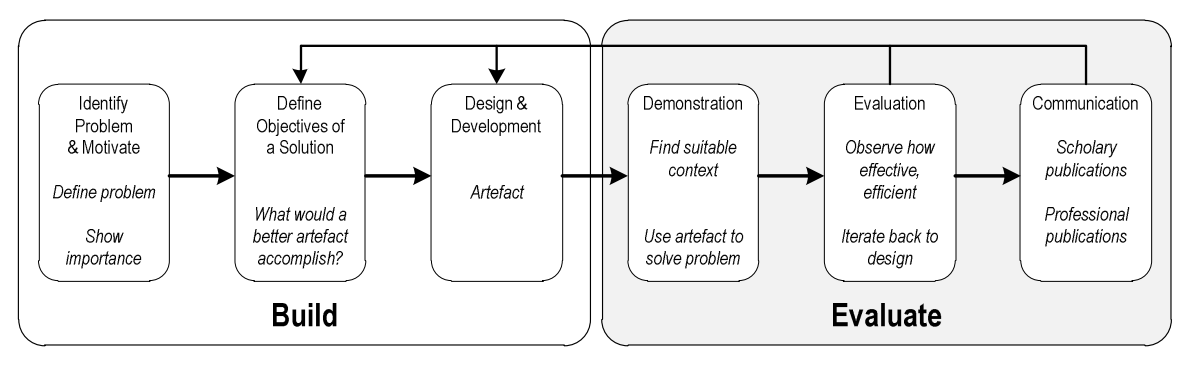
\includegraphics[width=1\linewidth]{chap3/images/dsr_process}
        \caption[DSR Process]{Design Science Research Approach according to Peffers et al.
        Picture:~\cite[p. 72]{sonnenberg2012evaluation}}
        \label{fig:dsr_process}
    \end{tcolorbox}
\end{figure}

\paragraph{``Activity 1 - Problem identification and motivation''~\cite[p. 52]{peffers2007design}:}
``Define the specific research problem and justify the value of a solution.''
~\cite[p. 52]{peffers2007design}

This study aims to improve the prediction of spring back in the air bending process using real world
data with supervised learning.
The value of the solution will be a reduction of trial and error cycles and therefore a reduction of time and cost in
the air bending process.
The problem as well as the motivation for this study was described in the \cref{ch:introduction}
``Introduction'' in more detail.

\paragraph{``Activity 2: Define the objectives for a solution''~\cite[p. 55]{peffers2007design}:}
The goal of a solution comes from the definition of the problem, which takes into account what is possible and feasible.
Objectives can be quantitative or qualitative, and they should be based on the problem specification that was
established in the previous step.
Knowledge about previous solutions and their effectiveness is required~\cite[p. 55]{peffers2007design}.

The objectives for the solution, the different \ac{ML} models, will be to excell in all six Design Principles which
will be introduced in the next chapter.
The Design Principles are a set of criteria that are used to evaluate the performance of the \ac{ML} models.

\paragraph{``Activity 3: Design and development''~\cite[p. 55]{peffers2007design}:}
In this phase, the development of the artifact takes place.
An artifact, which may encompass models, methods, or constructs, serves as a critical element in addressing the
research question.
The process begins with outlining the functionality and architecture of the artifacts, followed by their subsequent
creation~\cite[p. 55]{peffers2007design}.

In this study the artifacts are Machine Learning models.
This steps includes the model selection and the training of the models.
The development of the artifacts is described in the \cref{ch:build} ``Build''.

\paragraph{``Activity 4: Evaluation''~\cite[p. 56]{peffers2007design}:}
In this activity, the effectiveness of the developed artifact in addressing the defined problems from Activity 1 is
examined and assessed.
The evaluator is expected to have knowledge of relevant metrics and analytical techniques.
The evaluation process may vary based on the nature of the problem at hand which is Machine Learning in this
study~\cite[p. 56]{peffers2007design}.
A comparison between the functionality of the artifact and other existing solutions can be conducted.
Additionally, quantifiable parameters can be employed to objectively measure the artifact's
performance~\cite[p. 56]{peffers2007design}.
As already stated in this study the created artifacts are evaluated using six distinct design principles.

\cite{peffers2007design} note that researches are not obligated to follow the order of activities
from 1 to 6
~\cite[p. 56]{peffers2007design}.
In this study the order fo the activities 4 and 5 swapped, in the original DSR approach the evaluation is done after
the demonstration activity, this was changed because the evaluation activity is used to select the best performing
artifacts.
How the \ac{ML} models where evaluated is described in the \cref{sec:evaluation-of-machine-learning-models}.


\paragraph{Activity 5: Demonstration}
The purpose of this activity is to demonstrate the effectiveness of the previously created artifact in solving one or
more problems.
Effective knowledge of the artifact is necessary for this activity
~\cite[p. 55]{peffers2007design}.
Unlike the evaluation activity, which assesses the overall performance of the artifact, demonstration focuses on the
performance of the artifact in specific scenarios.
To achieve this, three scenarios, each comprising two examples (single spring back predictions), are utilized to
compare the best-performing models.
The scenarios are selected to cover the entire attribute space of the problem and are described in detail in
~\cref{ch:evaluation}, \textit{Evaluation}.

\paragraph{Activity 6 - Communication}
The last activity is ued to communicate significance of the problem and the usefulness of the artifacts to a wider
audience
~\cite[p. 56]{peffers2007design}.
In this study this is done in the \cref{sec:results-and-discussion} ``Results and Discussion''.


\section{Design Principles}\label{sec:design-principles}
Recent studies suggest that the desired result of design science endeavors should also be knowledge that takes the
shape of
\ac{DP}~\cite{baskerville2010explanatory, sein2011action, gregor2013positioning}.
They capture knowledge concerning the production of additional examples of objects that belong to the same
category
~\cite[p. 39]{sein2011action}.
Other ML models are examples of the same category in the context of this study.
This information is gathered as the researcher progresses from one instance of the artifact to a more general level
~\cite[p. 37]{chandra2016making}.

In this study \ac{DP}s should provide a set of guidelines for the creation of new artifacts.
% TODO weg weil ich es nicht in der Quelle gefunden habe...
%Also DPs should be abstract enough to be used in later research as well~\cite[p. 37]{sein2011action}.


\section{Evaluation of Machine Learning Models}\label{sec:evaluation-of-machine-learning-models}
The field of software engineering has established standards for determining the quality of software systems and their
components.
One such notable standard is the ISO/IEC 9126, which provides a quality model that is widely used in
software engineering.
These standards are not applicable for evaluating \ac{ML} models, as data-driven software components, such
as \ac{ML} models, have functionalities that is not fully defined by the developer but rather is learnt from data.
As a result, when compared to traditional software engineering, using ML poses unique issues.
~\cite[p. 2]{siebert2022construction}.
Therefore, as noted by~\cite{siebert2022construction}, adaptation is necessary.
They have reinterpreted and expanded upon these existing quality models to make them applicable to the context of
Machine Learning, as stated in their work
~\cite[p. 1]{siebert2022construction}.

In this study, in order to define the Design Principles for the \ac{ML} models in this work, the
considerations of~\cite[]{siebert2022construction} are used.
This allows for a systematic process to assess the quality of the developed models.
\cite{siebert2022construction} consider several quality attributes, including
correctness, relevance, robustness, stability, interpretability and resource utilization.
Alongside these attributes, the authors also provide a set of quality measures to evaluate the
models, but these are not complete and are only used as a starting point for the evaluation of the
models in this work, further evaluation is described in \cref{ch:evaluation}.


\section{Goal Question Metric Approach}\label{sec:goal-question-metric-approach}
To make the defined quality attributes measurable, the Goal-Question-Metric (\ac{GQM})-approach was chosen in this
study.
It is one of the most common approaches in DSR and is divided into three levels~\cite[p. 3]{van2002goal}.

\paragraph{1. Conceptual level (goal):}
``A goal is defined for an object, for a variety of reasons,
with respect to various models of quality, from various points of view, relative to a
particular environment.''
~\cite[p. 3]{van2002goal}

Specific goals are established for a software product (in this case a \ac{ML} model).
These goals consider various quality aspects, perspectives, and contexts.
Clearly defined goals help to guide the direction of the development
~\cite[p. 3]{van2002goal}.
In this study the goals are the Design Principles that are to be established in the next \cref{ch:build}.

\paragraph{2. Operational level (question):}
To achieve the set goals, one or multiple questions are formulated to assess and characterize the objectives.
These questions address the quality attributes and help to understand the object of measurement from the selected
viewpoint.
The questions guide the measurement process by identifying the relevant aspects that need to be
analyzed~\cite[p. 3]{van2002goal}.

\paragraph{3. Quantitative level (metric):}
For each question, a set of metrics is defined to provide quantitative data and answers.
These metrics are used to evaluate the object of measurement, offering precise and objective insights into the
quality aspects being assessed~\cite[p. 3]{van2002goal}.

In this study only one question is formulated for each goal.
The goals, questions and metrics are presented in the next chapter.

    % NOTES 
% Wie ich den sprinback gemssen habe 

\chapter{Build}

\section{Problem Statement} 
The following design principles is a selection of \cite{siebert_constructionqualitymodel_}'s quality parameters for \ac{ML} models.
In this \ac{DSR} work the artifacts are \ac{ML} models therefore these design principles are used to evaluate them.

\subsubsection*{Design Principle 1: Correctness}
\textit{Does the artifact predict the spring back of a sheet metal with a high accuracy and correctness?}
With progression in manufacturing there is a growing demand for high-quality products, that means that the meta parts needs to be produced with high precision and accuracy. Here the sprin back is an undesired side effect which need to be mimimized. \cite[p. 1]{baig_machinelearningprediction_2021}
Sheet metal forming in manufacturing need a high level of quality and precision. Therefore, the spring back of a sheet metal is an important parameter to consider. \cite[p. 1]{cruz_applicationmachinelearning_2021}
Predicting spring back is important to reduce the number of trial and error cycles in the manufacturing process.
Also predicting spring back is complex because of many variables and parameters and often not all of them are known. 
Therefore, a machine learning model should predict the spring back of a sheet metal with a high accuracy and correctness. When using the \ac{ML} model small errors in the prediction can cause fitting problems in the manufacturing process.

% Using an analytical model to compare the artifact. (miranda 2018 paper)

\subsubsection*{Design Principle 2: Appropriateness}
\textit{Is the artifact appropriate for the given problem?}
While selecting a model it is important that it fits the problem/task and can deal with the given data. \cite[p. 16]{siebert_constructionqualitymodel_}


\subsubsection*{Design Principle 3: Relevance}
\textit{Does the artifact achieve a good bias-variance trade-off?}

In addition to measure the correctness it is important to understand "why" the learner has this performance. 
This is important to understand the limitations of the model and to improve it. 
Therefore, it is important to understand the bias-variance trade-off. \cite[p. 50]{zhou_machinelearning_2021}
Bias measures the differences between the learnesrs expected prediction and the ground-truth label. This results in the fitting ability of the learner. 
Variances measures the change of learning performance of the learner because of changes in the training set. This results in the impact of data disturbance on the results. \cite[p. 51]{zhou_machinelearning_2021}

\subsubsection*{Design Principle 4: Robustness}
\textit{How well does the artifact handle outliers, noise and missing data?}

"Noise is common in any real-world data set and may adversely affect classifiers built under the effect of
such type of disturbance. Some of these classifiers are widely recognized for their good performance
when dealing with imperfect data. However, the noise robustness of the classifiers is an important issue
in noisy environments and it must be carefully studied. Both performance and robustness are two
independent concepts that are usually considered separately, but the conclusions reached with one of
these metrics do not necessarily imply the same conclusions with the other. Therefore, involving both
concepts seems to be crucial in order determine the expected behavior of the classifiers against noise.
Existing measures fail to properly integrate these two concepts, and they are also not well suited to
compare different techniques over the same data. This paper proposes a new measure to establish the
expected behavior of a classifier with noisy data trying to minimize the problems of considering
performance and robustness individually: the Equalized Loss of Accuracy (ELA)."


\subsubsection*{Design Principle 5: Stability}
\textit{Does the artifact generate repeatable results when trained on different datasets?}


\subsubsection*{Design Principle 6: Interpretability}
\textit{Is the artifact easy to understand and explain?}

It should be noticed, that there are many parameters and variables involved in the sheet metal forming process. 
That makes the process design quite complex, particularly in the production of components which require several stages, and thus more than one set of tools. \cite[p. 1]{dib_singleensembleclassifiers_2020}
A model which allows conclusions how the results where generated is better.

\subsection*{Design Principle 7: Resource utilization}
\textit{How many resources does the artifact need to train and predict?}

Conventional processes are often based on empirical trial and error approaches. \cite[p. 1]{dib_singleensembleclassifiers_2020}
A common approach is to experimentally create so named 'technology tables' which contain the bending parameters and the resulting spring back. (Quelle: Hochstrate?)
This process is time and cost intensive and therefore often not suitable for the production of high-volume and low-cost components.
Therefore, one of the benefits of using machine learning should be the reduction of the number of trial and error cycles in the manufacturing process. 
Furthermore, training the model should take not too much time and resources.
As mentioned before often FEM-simulation are used to virtually try out metal forming processes. However, fully exploring the design space is computationally expensive and often not possible. \cite[p. 3]{dib_singleensembleclassifiers_2020} 
The number of experiments can be reduced using a meta-model like \ac{ANN}. \cite[p. 3]{dib_singleensembleclassifiers_2020}
A approach fully based on \ac{ML} should perfor



\section{Dataset generation}
For the dataset generation, bending experiments were performed on metal sheets with different thicknesses.
% material
The material used is cold rolled steel sheets of the norm DIN EN 10130. The thicknesses used were 0.5mm, 1mmm and 2mm.
The material was used because it is commonly used in bending processes and its high availability. In previous tests, it was observed, that the spring back are well observable with this material.
Using this material, 200 single bending pieces of the dimension 20×100 mm have been cut.
Each piece was bend one time using a \textit{Zwick} three-point-bending machine.

Python script where developed to covert the output data format from the machine to CSV files.
The following describes the experimental setup used for the experiments performed.

\subsection{Preliminary Tests}
A number of preliminary tests were conducted to determine the influence of the punch penetration on the spring back.

\subsubsection{Multiple Cycles}
One approach was to test if multiple spring back can be measure using only one sheet.
Therefore, the machine was programmed to perform multiple cycles in one attempt and bend the metal sheet multiple times. The benefit of this approach would have been a faster generation of the dataset because spring backs could be measured in on attempt, also less material would have been used.

Figure~\ref{springback_multiple} shows one of these attempts. The metal sheet was bent 4 times using $y_p$ values from 5 to 8. The results show, that 4 different spring backs can be measured, but the spring back does not vary like expected. It was observed as well, that the spring backs are different in every attempt, this is shown in Figure~\ref{springback_multiple_inconsistent_results}.
Bending 4 different metal sheets each only one time returned very different results.
A possible explanation could be the cold deformation of the steel, which is not reversible. Because this approach did not work, the machine was programmed to perform one cycle at a time.

\captionsetup{width=0.45\textwidth}

\begin{figure}[H]
    \centering
    \begin{minipage}[b]{0.5\textwidth}
        \centering
        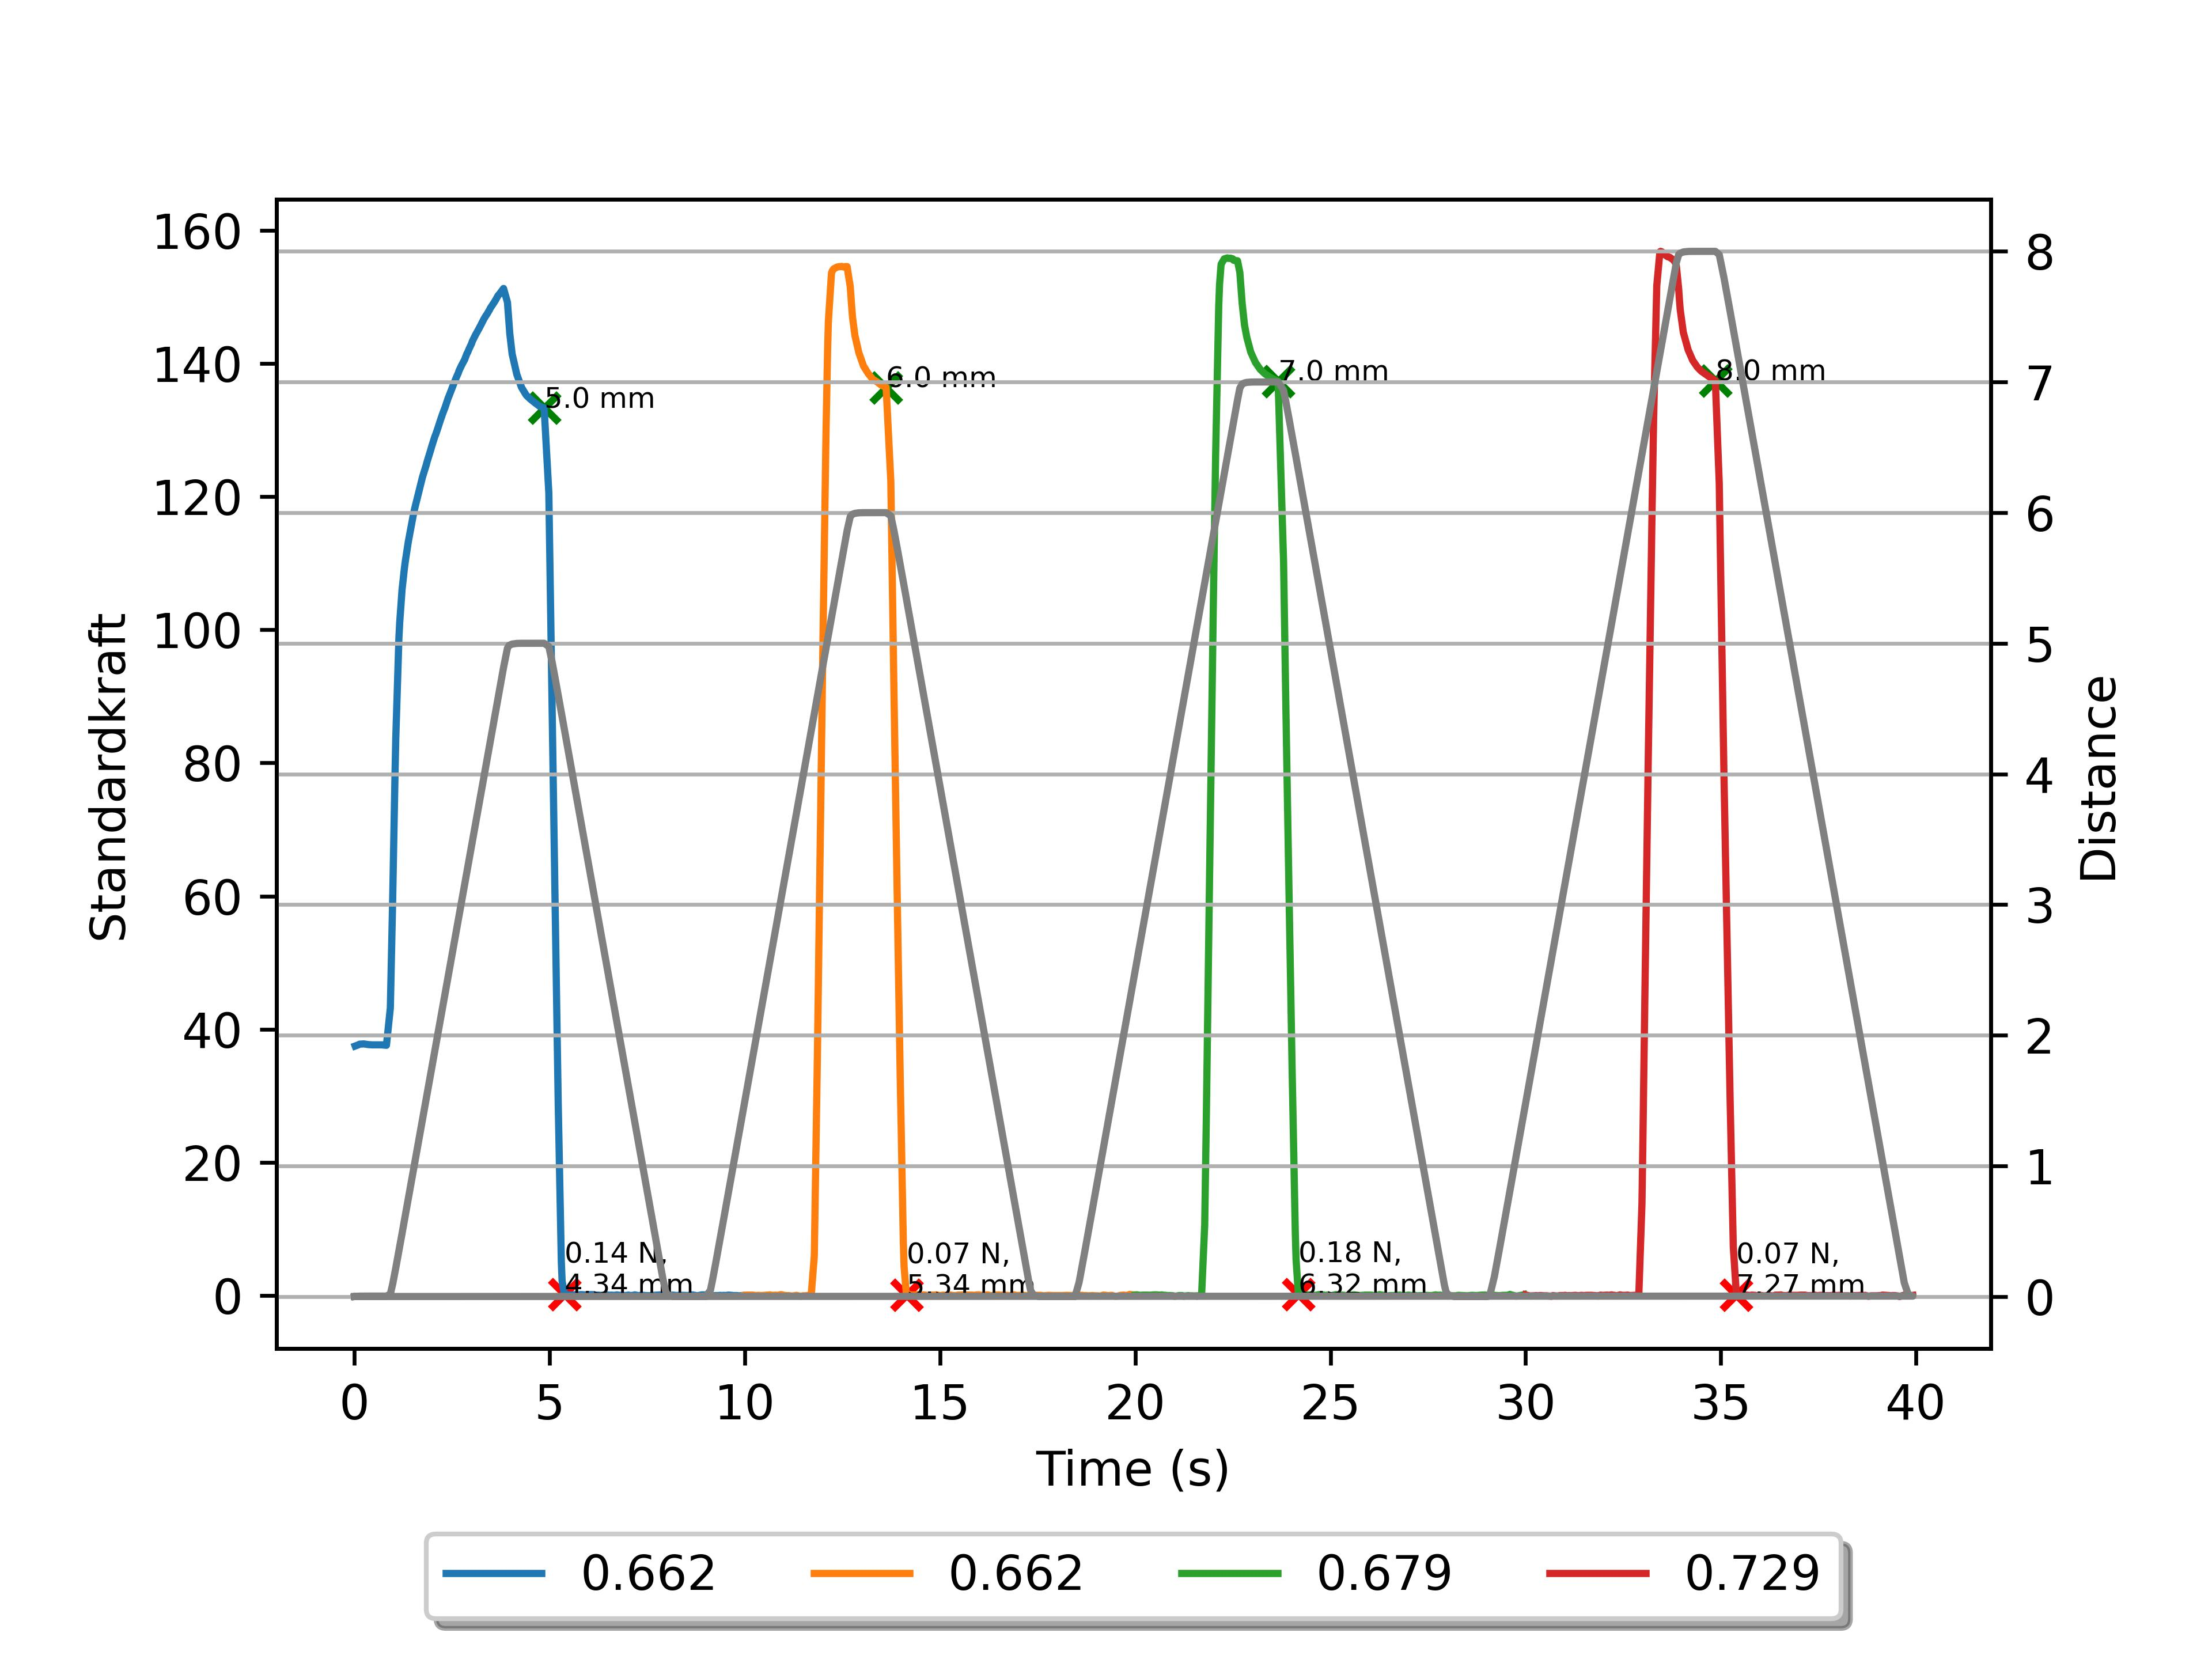
\includegraphics[width=0.9\textwidth]{springback_multiple.jpg} % first figure itself
        \caption{Experiment: Bending one metal sheet multiple times with different $y_p$ values.}
        \label{springback_multiple}
    \end{minipage}\hfill
    \begin{minipage}[b]{0.5\textwidth}
        \centering
        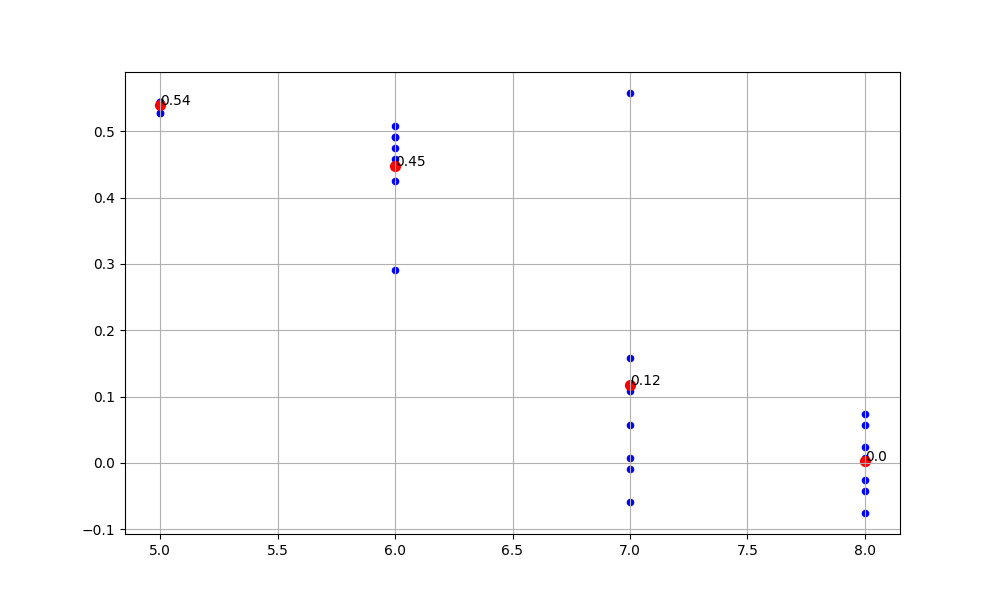
\includegraphics[width=1.1\textwidth]{springback_multiple_inconsistent_results.png} % second figure itself
        \caption{Inconsisten results bending one metal sheet mutliple times. The spread of the results is very large.}
        \label{springback_multiple_inconsistent_results}
    \end{minipage}
    \label{fig:springback_multiple_overview}
\end{figure}

\subsubsection{Brake Bending Machine}
Before using the three point bending machine, a brake bending machine was used to test the influence of the bending on the spring back. The brake bending machine is a machine used to bend metal sheets. It is a very common machine in the industry and is used to bend metal sheets to a specific radius. The brake bending machine used is a \textit{Bendmaster 1000} from \textit{Bendmaster}.

After a series of bends it was observed, that the spring back values where much higher than expected. The explanation for that behavior was, that altering the position the bending beam of that specific machine was not enough to get the desired angle. Thus, the machine excluded for the generation of the data and the three point bending machine was used instead.

Despite the inaccurate data, it was later observed, that the distribution of the spring backs was very similar to the later experiments with the three point bending machine.


\subsection{Experimental setup}
The setup consists of a three-point-bending machine with a punch and a die with no bottom. The machine used is the \textit{Zwick MX 25A} material testing machine.
The machine is equipped with a load cell and a displacement sensor. The load cell is used to measure the force applied to the sheet and the displacement sensor is used to measure the displacement of the punch.
The machine is controlled by a computer and a software called \textit{ZwickRoell TestXpert}. The software is used to control the machine and to save the output data.

The experimental setup and the process parameters are shown in Figure~\ref{fig:setup} where $V$ is the die opening, $y_p$ is the punch penetration which is the distance the punch is moved into the sheet.
The paramter $t$ is the sheet thickness,  $\alpha$ is the sheet corresponding bending angle. Parameter $r_p$ is the punch radius which is the radius of the tip of the punch and $r_m$ is the die radius.


\begin{figure}[H]
    \centering
    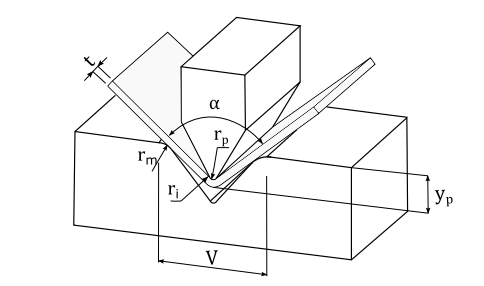
\includegraphics[width=0.6\textwidth]{setup}
    \caption{Process parameters: Sheet bending angle ($\alpha$), sheet thickness ($t$), punch penetration ($y_p$), die opening ($V$), punch radius ($r_p$), die radius ($r_m$), inside bending radius ($r_i$).}
    \label{fig:setup}
\end{figure}

In order to get consistent results, a number of constant and variable parameters were chosen.
The parameters include the punch-and-die tooling made of steel where die punch had a radius ($r_p$) of 5 mm and and die radius ($r_m$) of 10 mm. The die opening $V$ was varied between 10 and 50 mm and the punch penetration $y_p$ was varied between 0 and 20 mm.
The machine was configured to move the punch with a constant speed of 100 mm/min until it measured a resistance of 1 N. That meant, that the punch reached the metal plate and the actual bending process can start. After a hold time of 1 second the punch was moved with a slower speed of 8 mm/min until the specified punch penetration was reached.
The length and width of the metal sheet was 100 mm and 20 mm respectively. The sheet thickness was varied between 0.5 and 3 mm.
The constant parameters are shown in Table~\ref{tab:constant_parameters} and the varying parameters are shown in Table~\ref{tab:verying_parameters}.

\begin{table}[H]
    \centering
    \begin{tabular}{|l|l|l|}
        \hline
        \textbf{Parameter} & \textbf{Value}                      & \textbf{Unit} \\ \hline
        Punch penetration  & 2.5, 5, 7.5, 10, 12.5, 15, 17.5, 20 & mm            \\
        Die opening        & 10, 20, 30, 40, 50                  & mm            \\
        Thickness          & 0,5, 1, 1.5, 2, 2.5, 3              & mm            \\
        \hline
    \end{tabular}
    \caption{Experimental setup varying parameters}
    \label{tab:verying_parameters}
\end{table}

\begin{table}[H]
    \centering
    \begin{tabular}{|l|l|l|}
        \hline
        \textbf{Parameter}            & \textbf{Value} & \textbf{Unit} \\ \hline
        Punch radius                  & 5              & mm            \\
        Die radius                    & 5              & mm            \\
        Sheet thickness               & 0.5, 1, 2      & mm            \\
        Sheet width                   & 20             & mm            \\
        Sheet length                  & 100            & mm            \\
        Punch speed                   & 100            & mm/min        \\
        Punch speed after penetration & 8              & mm/min        \\
        Punch force                   & 1              & N             \\
        \hline
    \end{tabular}
    \caption{Experimental setup constant parameters}
    \label{tab:constant_parameters}
\end{table}


\subsection{Measuring The Spring Back}
The output data contained different data points, which were used to calculate the spring back.
Important parameters for the calculation are the force, punch penetration and testing time.
As shown in Figure~\ref{fig:springback_measured} at the $yp$ maximum the punch penetration and the force are maximized as well. The punch stays at that position for 1 second and then moves back with a slower speed. This hold time a limitation of the machine and can not be changed.
After the punch is moved back, the force is reduced and the punch penetration is reduced as well, until the punch is at the initial position. For a short time after the lift, the load  cell still measures a force. That is because the metal sheet springs back and the punch is still in contact with the sheet. This was measured using a python script, the green and the yellow point represent the resulting spring back distance.

\begin{figure}[H]
    \centering
    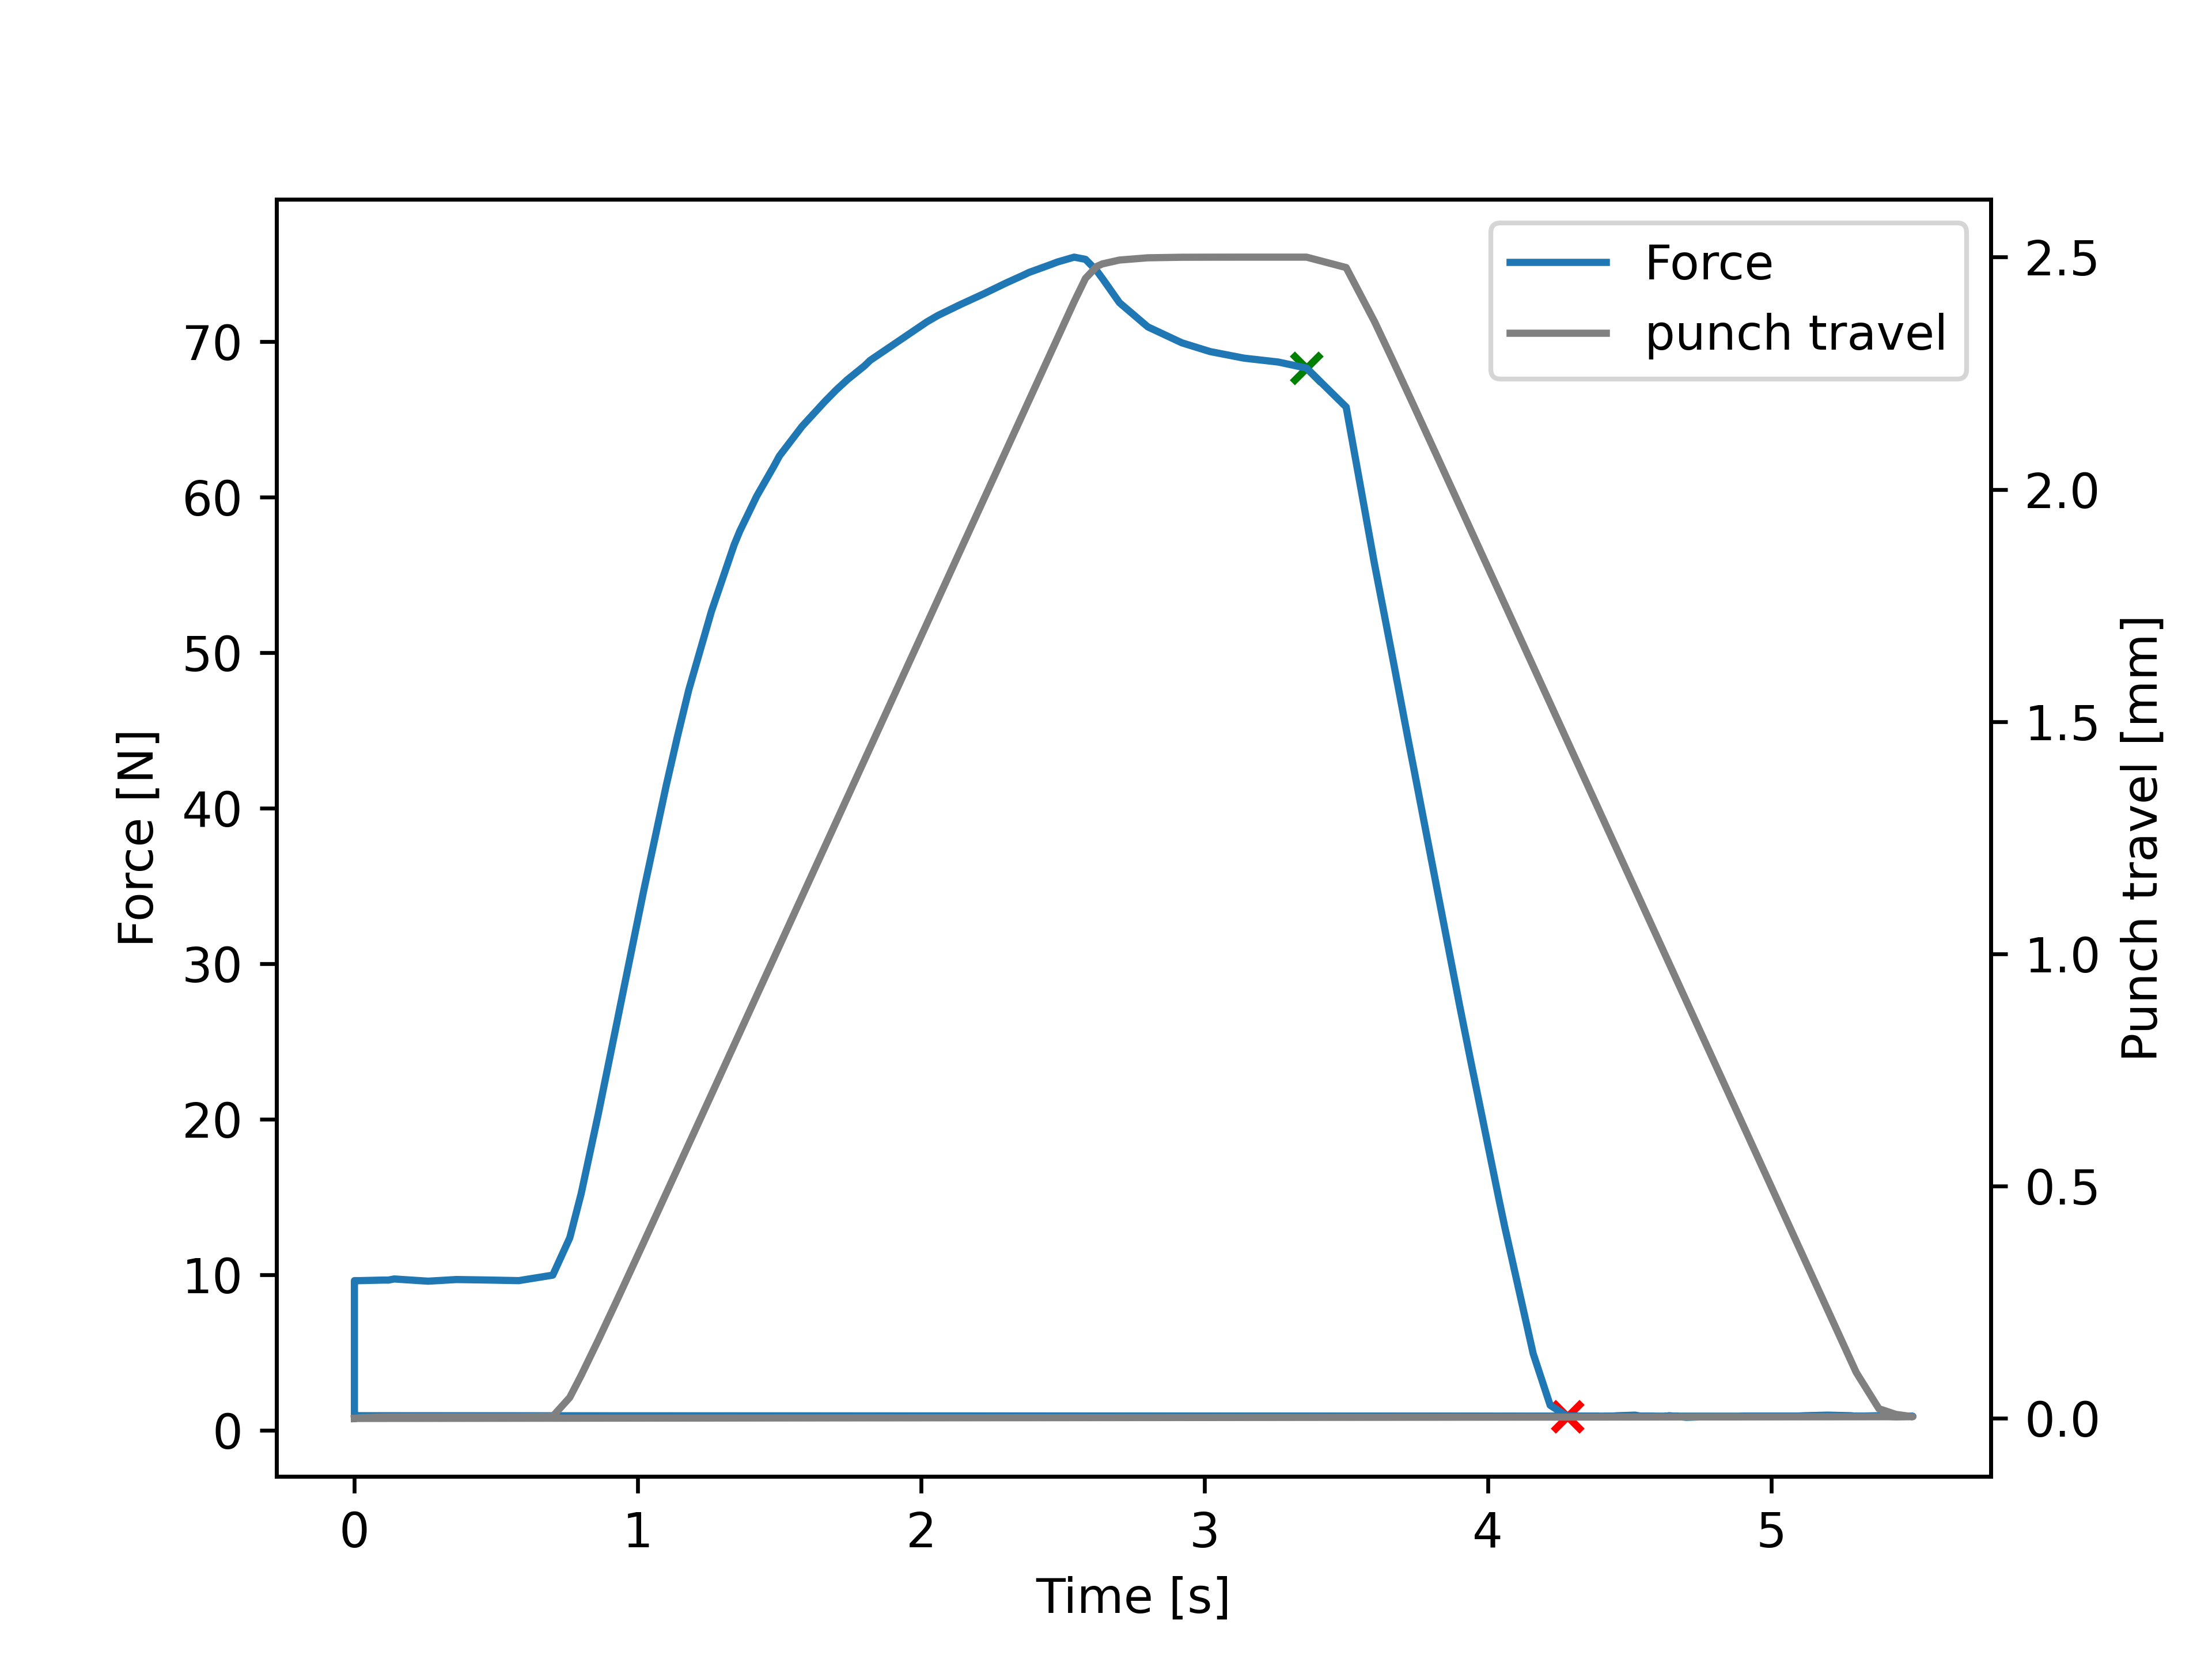
\includegraphics[width=0.6\textwidth]{springback_measured}
    \caption{A steel metal sheet was bent with a punch penetration of 5 mm the spring back is 0.37 mm. The blue line shows the force and the blue line shows the punch penetration.}
    \label{fig:springback_measured}
\end{figure}

% \paragraph{Bend deduction:}
% Measuring the bend deduction is more complex. After a metal sheet is bent, it is hard to measure the flat pattern length because the material is malformed at the bent. 
% As a result, the neutral axis is not in the center of the sheet and hard to measure, but it can be calculated using different approaches. %quelle und ausführlicher und grunlagen teil  
% There are multiple ways to measure the bend deduction described earlier. 
% % K-Faktor Muss noch in theorie teil 
% In this setup, the method described in the DIN6395 was used. This method uses a k-factor which is an approximated value and therefore and therefore it can be inaccurate. (Equation~\ref{eq:kfactor}). % cite DIN norm 

% \begin{equation}\label{eq:kfactor}
%     k=0.65+\frac{1}{2}\log{\frac{r}{s}}
% \end{equation}

% \begin{figure}[ht!] % supposedly places it here ...
% 	\centering
% 	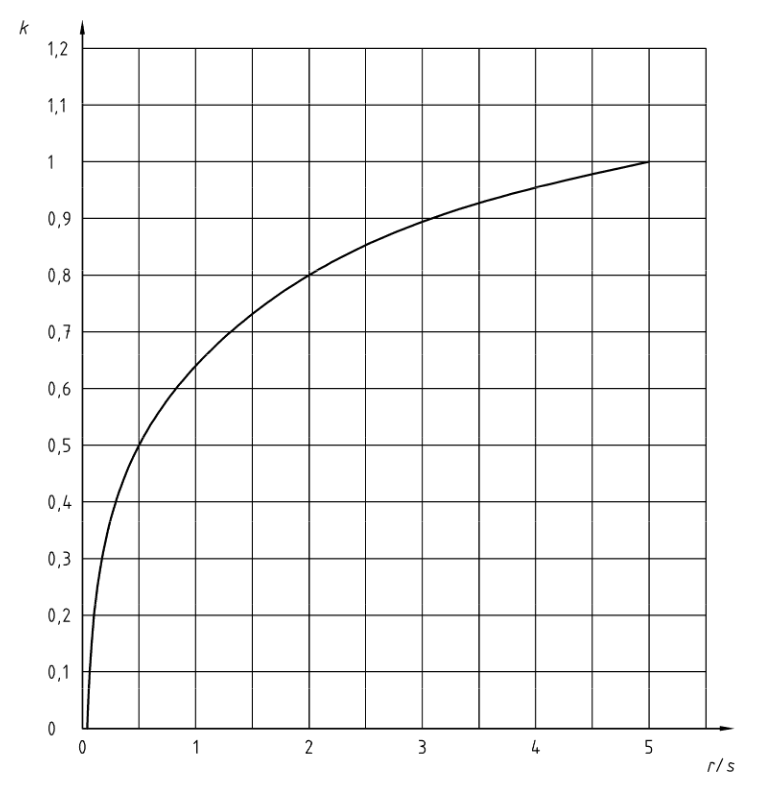
\includegraphics[width=0.5\linewidth]{k-factor}
% 	\caption[Graphical representation of the correction factor]{Graphical representation of the correction factor.}
% 	\label{fig:test1}
% \end{figure}

% The DIN 6935 used the formula for the stretched length, $length=a+b+v$ where \textit{a} and \textit{b} are the side lengths of the sheet and \textit{v} is a correction value for the deduction. \cite{din6935}
% The stretched length is measured different depending on the bending angle.

% \paragraph{Opening angle $\beta 0^\circ$ to $90^\circ$} 
% For opening angles between $0^\circ$and $90^\circ$ the side lengths \textit{a} and \textit{b} are dimensioned from the tangent of the bend to the edge. 
% To calculate the compensation value \textit{v} (Equation~\ref{eq:v1}) is used
% \cite{din6935}.

% \begin{equation}\label{eq:v1}
%         v=\pi*(\frac{180^\circ-}{180^\circ})*(r+\frac{s}{2}*k)-2(r+s)
% \end{equation}

% \begin{figure}[H]
% 	\centering
% 	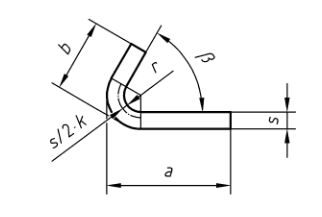
\includegraphics[width=0.5\linewidth]{bending-angle-90}
% 	\caption[Opening angles $\beta 0^\circ$ to $90^\circ$]{Opening angles $\beta 0^\circ$ to $90^\circ$ \cite{din6935}}
% 	\label{fig:v1-image}
% \end{figure}

% \paragraph{Bending angle $\beta90^\circ$ to $165^\circ$} (Equation~\ref{eq:v1})
% For opening angles between $90^\circ$ and $165^\circ$ the side lengths \textit{a} and \textit{b} are dimensioned from the apex to the edge. 
% To calculate the compensation value \textit{v} (Equation~\ref{eq:v1}) is used. 
% \cite{din6935}

% \begin{equation}\label{eq:v2}
%     v=\pi*(\frac{180^\circ-}{180^\circ})*(r+\frac{s}{2}*k)-2(r+s)+\tan{\frac{180^\circ-\beta}{2}}
% \end{equation}

% \begin{figure}[!ht]
% 	\centering
% 	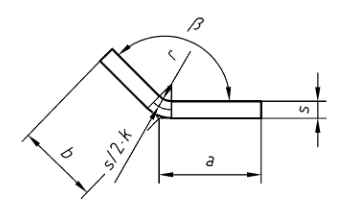
\includegraphics[width=0.5\linewidth]{bending-angle-165}
% 	\caption[Opening angles $\beta90^\circ$ to $165^\circ$]{Opening angles $\beta90^\circ$ to $165^\circ$ \cite{din6935}}
% 	\label{fig:v2-image}
% \end{figure}

% For opening angles between $165^\circ$ and $180^\circ$ the compensation value \textit{v} is 0. The values for v would be negligibly small. \cite{din6935} The side lengths \textit{a} and \textit{b} where measured using the software \textit{ImageJ}. 

% Edge cracking is not measured for now because the steel used has no high-strength and with machine in usage it was not possible to create edge cracking.

% \begin{figure}[!ht]
% 	\centering
% 	\includegraphics[width=0.5\linewidth]{example-image}
% 	\caption[Screenshot ImageJ]{Screenshot ImageJ}
% 	\label{fig:imagej-screenshot}
% \end{figure}


\subsection{Computational Setup}
For training the machine learning models a ThinkPad X1 Carbon 2019 with an Intel Core i7-10610U CPU @ 1.80GHz and 16 GB RAM was used. The operating system used is Ubuntu 20.04.2 LTS. The code for the model is written in Python 3.8.5 using the IDE PyCharm The libraries used are mentioned in Table

\captionsetup{width=1\textwidth}

\begin{table}[H]
    \centering
    \begin{tabular}{|ll|}
        \hline
        \textbf{Library} & \textbf{Version} \\
        \hline
        numpy        & 1.23.2  \\
        pandas       & 1.5.1   \\
        matplotlib   & 3.6.2  \\ \hline 
    \end{tabular}
    \label{table:libraries}
    \caption{Libraries used for the machine learning models.}
\end{table}

\subsection{Data Preprocessing}
% "Although the dataset collected from the experimental setup includes seven features (parameters), the 
% first three parameters; load tonnage, load holding time, and gap between the punch and the die, are 
% combined to form a single feature, "Machine". It is because different combinations of these factors may 
% be combined to form a single machine setting parameters. The other parameters are; blank material, 
% thickness, width and initial bend angle. Hence, there are five features of the dataset, which levels are 
% shown in Table 4. Two of which, namely machine and material, are treated as categorical features, so 
% using scikit-learn's OrdinalEncoder these features were encoded into an integer array. While the 
% remaining three features were treated as continuous features, for standardizing these features scikit-
% learn's StandardScaler was used. It transformed the data so that for each feature, its distribution 
% will have a mean value of 0 and a standard deviation of 1. The formula used for this is as follows Eq 
% (1)." 
% \cite[p. 7]{baig_machinelearningprediction_2021}

\section{Model Selection}

\begin{itemize}
    \item Multi-layer Perceptron (MLP)
    \item Decision Tree (DT)
    \item Random forest (RF)
    \item Naive Bayes (NB)
    \item Support vector machine (SVM)
    \item K-Nearest neighbors (KNN) 
    \item Logistic Regression (LR)
\end{itemize}

\section{Model Training}









    \chapter{Evaluation}\label{ch:evaluation}
% take a step back and put your results from 4 into context. 
This chapter conducts a comprehensive analysis of the \ac{ML} models implemented in
the preceding chapter.
An overview of the quality metrics used for the evaluation is presented in
Table~\ref{tab:evaluation_criteria}.
The quality metrics have been structures based on
the \ac{GQM}approach mentioned in subsection~\ref{subsec:goal-question-metric-approach}.

The quality metrics are aligned with the quality model
from~\cite{siebert2022construction}, which in turn is based on the ISO/IEC 9126 standard for
software quality evaluation.
The standard has been adapted by \cite{siebert2022construction} to meet the specific
requirements of machine learning models, as described in section~\ref{sec:evaluation-of-machine-
learning-models}.

As~\cite{siebert2022construction} mostly focuses on the evaluation of classification
models, the quality metrics have been adapted to fit the requirements of the regression
models implemented in this thesis.
This is elaborated in each individual quality metric section.

Table~\ref{tab:evaluation_criteria} shows the quality metrics used for the evaluation
of the \ac{ML} models.
The \ac{GQM} approach is used to structure the evaluation of the \ac{ML} models.
To each goal a question or one or more metrics where assigned.
The following subsections follow this structure and describe the quality metrics in more
detail.

\captionsetup{margin={5pt,5pt}}
\begin{table}[{}]
    \begin{tcolorbox}[arc=0pt,boxrule=0.5pt]
        \centering
        {\renewcommand{\arraystretch}{1}
            \begin{tabular}{p{2cm}p{8cm}p{3cm}}
                \toprule
                \thead{\textbf{Goal}} & \thead{\textbf{Question}}
                & \thead{\textbf{Metric}} \\
                \toprule
                \textbf{Correctness} & Ability of the model to perform the
                current task measured on the development dataset and the runtime dataset~\cite[p
                . 16]{siebert2022construction}
                &
                MAE, \newline MSE, \newline RMSE
                \\
                \hdashline
                \textbf{Relevance} & Does the model achieve a good bias-variance
                tradeoff? Which means neither overfitting or unterfitting the
                data.~\cite[p. 16]{siebert2022construction}
                & Variance of CV, \newline $R^2$
                \\
                \hdashline
                \textbf{Robustness} & Ability of the model to outliers, noise
                and other data quality issues~\cite[p. 16]{siebert2022construction}
                & Loss of Accuracy, \newline Average Loss
                \\
                \hdashline
                \textbf{Stability} & Does the artifact generate repeatable
                results when trained on different data?~\cite[p. 16]{siebert2022construction}
                & LOOCV stability
                \\
                \hdashline
                \textbf{Interpret- ability} & How well can the model be
                explained?~\cite[p. 16]{siebert2022construction}
                & Linearity, \newline monotonicity, \newline  interaction
                \\
                \hdashline
                \textbf{Resource utilization} & How much resources are
                required to train and run
                the model?~\cite[p. 16]{siebert2022construction}
                & Training time, \newline runtime, \newline storage space
                \\
                \bottomrule
            \end{tabular}
        } % renew command
    \end{tcolorbox}
    \caption{Overview of the goals, questions and metrics for the
    evaluation of artifacts
    following the \ac{GQM} approach.}
    \label{tab:evaluation_criteria}
\end{table}


\section{DP1: Correctness}\label{sec:dp1:-correctness}
% Ability of the model to perform the current task measured on the
% development dataset and the
% runtime dataset

The model must be able to perform well on the selected task.
\cite{siebert2022construction} used the classification metrics precision, recall and F-
score to evaluate the correctness models.
As the regression models implemented in this thesis are not able to predict
the class of a sample, these metrics are not applicable.

Commonly used metrics for regression models are the mean absolute error \ac{MAE},
\ac{MSE} and \ac{RMSE}.
Their formal description is given in~\ref{eq:mae},~\ref{eq:mse} and~\ref{eq:rmse} where
\(e_i\) being the prediction error which is the difference between the predicted value
by the model and the acutal value.
\(y_i\) is the actual value and \(n\) is the number of samples in the testing data set.

For the evaluatoins the \texttt{sci-kit learn}~(\cite{scikit-learn}) implementation of
these metric was
used.

\textbf{Mean Absolute Error (MAE)}

\begin{tcolorbox}[arc=0pt,boxrule=0.5pt]
    \begin{equation}
        MAE = \frac{1}{n} \sum_{i=1}^{n} |e_i|
        \label{eq:mae}
    \end{equation}
\end{tcolorbox}

The MSE is the average of the squared differences between the predicted and
the actual values.
The MSE is more sensitive to outliers than the MAE.

\textbf{Mean Squared Error (MSE)}

\begin{tcolorbox}[arc=0pt,boxrule=0.5pt]
    \begin{equation}
        \label{eq:mse}
        MSE = \frac{1}{n} \sum_{i=1}^{n} e^2
    \end{equation}
\end{tcolorbox}

The RMSE is the square root of the MSE. The RMSE is the most popular metric
for evaluating the
performance of regression models. The RMSE is interpretable in the same units
as the response
variable. The RMSE is more sensitive to outliers than the MAE.
The MAE is the average of the absolute difference between the predicted and
actual values.

\textbf{Root Mean Squared Error (RMSE)}

\begin{tcolorbox}[arc=0pt,boxrule=0.5pt]
    \begin{equation}
        \label{eq:rmse}
        RMSE = \sqrt{MSE}
    \end{equation}
\end{tcolorbox}

For a full overview about the performance all three metrics are sued for the
evaluation.

% \subsection{Goal Hierarchy}

% The correctness describes the ability of the model to perform on the
% selected task. Concrete,
% the model has to predict the spring back as correct as possible. The goal
% hierarchy for the
% correctness is shown in Figure~\ref{fig:goal_hierarchie_correctness}.

% \begin{figure}[H]
%     \centering
%     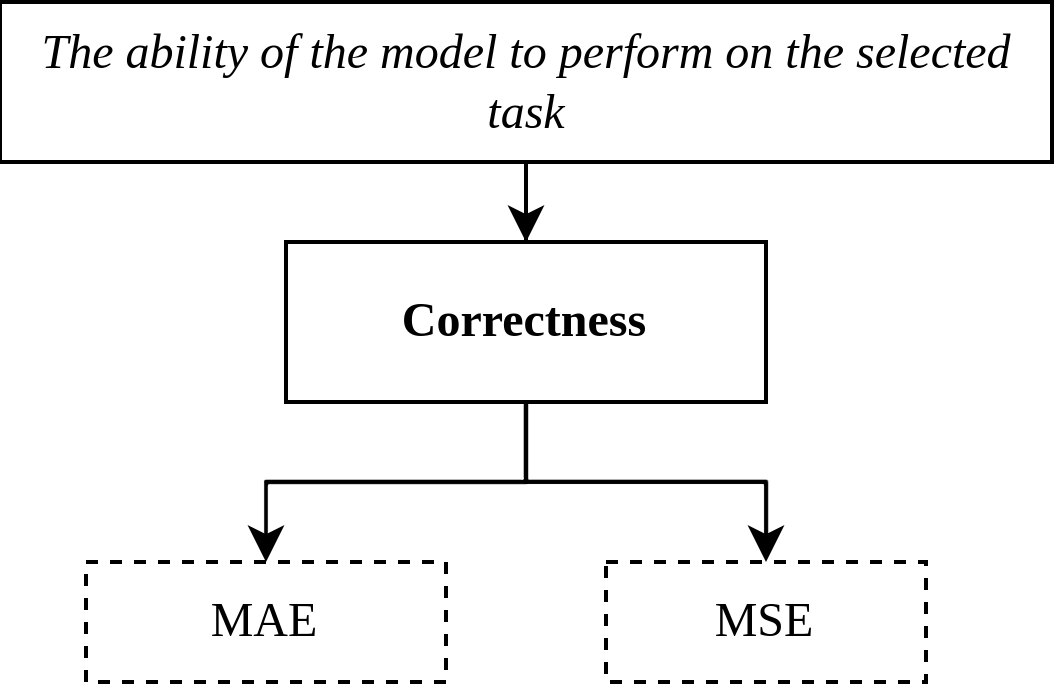
\includegraphics[width=0.6\textwidth]{goal_hierarchie_correctness}
%     \caption{Goal hierarchy: Correctness}
%     \label{fig:goal_hierarchie_correctness}
% \end{figure}

\subsection{Results}\label{subsec:results}
The Table~\ref{tab:results-correctness} shows the results of the
evaluation of the models for the correctness.

Looking at the \ac{RMSE} all models except the \ac{LR} and \ac{DC} models show a
relatively equal performance.
The \ac{MLP} has a slight advantage over the other models, with an \ac{RMSE} of 0.201.
Therefore it could be interesting to investigate the performance of neural networks /
deep learning in the future.

It's worth mentioning that the \ac{SVM} model has a slightly better \ac{MAE}, while
still maintaining a comparable \ac{MSE} compared to the other models.
This could be due to the fact that the errors made by the \ac{SVM} are evenly
distributed across instances, or that the errors made by the other models are large for
a few instances but smaller for the rest.

The algorithms \ac{LR} does perform worse than the other models.
A likely reason is, that the relationship between the independent and dependent
variables is not linear.
This can result in an inadequate fit and reduced predictive power (Source).

\ac{DT} on the other hand, can perform poorely when they overfit the training data.
Also, they are pron to instability, both problems are mitigates by using ensemble methods
like \ac{RF} and \ac{GBT} which can overcome the limitations of individual
decision trees.

Because the simple \ac{DT} as well as the \ac{LR} are not able to predict the
spring back correctly, they are not considered for the next steps of the evaluation.

% Table wit hall used machine learning models and their metrics
\begin{table}[H]
    \begin{tcolorbox}[arc=0pt,boxrule=0.5pt]
% \sisetup{group-minimum-digits = 4}
        \centering
        \begin{tabular}{llll}
            \toprule
            \thead{\textbf{Model Name}} & \thead{\textbf{MAE}}
            & \thead{\textbf{MSE}}
            & \thead{\textbf{RMSE}} \\
            \toprule
            \textbf{LR}  & 0.199 & 0.092 & 0.303 \\
            \hdashline
            \textbf{DT}  & 0.193 & 0.076 & 0.266 \\
            \hdashline
            \textbf{RF}  & 0.183 & 0.060 & 0.244 \\
            \hdashline
            \textbf{ET}  & 0.126 & 0.040 & 0.201 \\
            \hdashline
            \textbf{AB}  & 0.163 & 0.040 & 0.209 \\
            \hdashline
            \textbf{GBT} & 0.189 & 0.058 & 0.242 \\
            \hdashline
            \textbf{SVM} & 0.09  & 0.04  & 0.20  \\
            \hdashline
            \textbf{MLP} & 0.114 & 0.041 & 0.201 \\
            \bottomrule
        \end{tabular}
        \caption{Overview of the used machine learning models and their
        metrics.}
        \label{tab:results-correctness}
    \end{tcolorbox}
\end{table}


\section{DP2: Relevance}\label{sec:relevance}
% Does the model achieve a good bias-variance tradeoff? Which means neither
% overfitting or
% unterfitting the data.

% Bias variane trade-off
A model is considered relevant when it achieves a balance between bias and
variance, avoiding both overfitting and underfitting of the training data.
The relevance of the model can be quantified through the \textit{variance of
cross-validation}, which proves insight into how the model performs when trained and
evaluated on different subsets of data and how generalizes.

% Explanation interpretation of variance
A low variance indicates that the model's performance is consistent across
different folds,suggesting that the model is not overfitting the training data.
Conversely, a high variance implies that the performance can vary significantly
depending on the specific data points used the test set, indicating a potential
overfitting problem.

Figure~\ref{fig:variance-of-cv} shows how the variance of cross-validation
was calculated.
The parameter \(E\) denotes to the estimator which is used to calculate the
\ac{CV} score.
The parameter \(k\) denotes to the number of folds, which was set to 5 in this
context.
As estimator for the trained models \(R^2\) was used.
The \(R^2\) is a statistical measure of how close the data are to the fitted regression
line.

\begin{figure}[h]
    \begin{tcolorbox}[arc=0pt,boxrule=0.5pt]
        \centering
        \includegraphics[trim=left botm right top, width=0.9\textwidth]
        {chap5/images /cross_validation}
        \caption{Variance of cross-validation}
        \label{fig:variance-of-cv}
    \end{tcolorbox}
\end{figure}

\begin{equation}
    \label{eq:r2}
    R^2 = \frac{Explained\_variance}{Total\_variance\_targert\_variable}
\end{equation}

The value of the \(R^2\) is the percentage of the response variable variation that is
explained by a linear model.
It returns a score between 0 and 1, where 0 means that the model does not
explain any of the variance in the response variable around its mean, and 1 means that
the model explains all the variance in the response variable around its mean~\cite[p.
43]{muller_introductionmachinelearning_2016}.
Special in sci-kit learns implementations is that the score can be negative if the model
performs poorly.
If a model always predicts the expected value of y, regardless of the
input features, it would receive an R^2 score of 0.0~\cite{_sklearnmetricsr2_}.

Therefore, a high \(R^2\) indicated a good model fir and good bias-variance
tradeoff\cite[p. 43]{muller_introductionmachinelearning_2016}.

\subsection{Results}\label{subsec:results3}

Table~\ref*{tab:results_relevance} shows the variance of cross-validation
and the \(R^2\) for all used machine learning models.
To calculate the variance of cross-validation the variance of Scikit-Learn's
\texttt{cross\_val\_score} was calculated.
Five-fold cross-validation was used to calculate the variance of
cross-validation.
The \(R^2\) was calculated with the formula~\ref{eq:r2}.

It can be observed that most of the models have relatively low variance, indicating
consistent performance across different folds, however, two models stand out - \ac{GBT}
and ac{MLP}.

For the \ac{GBT} model, the variance is high, which implies that its performance
fluctuates significantly across different folds.
This inconsistency is a typical sign of overfitting, where the model is overly complex
and has learned the noise in the data rather than the underlying pattern.
The individual cross-validation scores for the GBT model also confirm this assumption,
with a negative score on the first fold and relatively high scores on the subsequent
folds.
Given this poor performance, the GBT model cannot be considered relevant for the given
task.

Similarly, the \ac{MLP} model has a relatively high variance score, which suggests that
its performance also fluctuates across different folds. The individual scores for the MLP
model show that it performs poorly on a few folds.

This performance inconsistency could be due to either overfitting or high variability
in the data.

Overall, it's important to consider the cross-validation scores in conjunction with
the other other metrics to get a more complete picture of how well your model is
performing.
This will be done in later sections.

\begin{table}[H]
    \begin{tcolorbox}[arc=0pt,boxrule=0.5pt]
% \sisetup{group-minimum-digits = 4}
        \centering
        \begin{tabular}{llll}
            \toprule
            \thead{\textbf{Model Name}} & rs & \thead{\textbf{Variance of CV}}
            & \thead{\textbf{\(R^2\)}} \\
            \toprule
            \textbf{RF}  & - & 0.068 & 0.8   \\
            \textbf{RF}  & x & 0.071 & 0.805 \\
            \hdashline
            \textbf{ET}  & - & 0.064 & 0.832 \\
            \textbf{ET}  & x & 0.352 & 0.82  \\
            \hdashline
            \textbf{GBT} & - & 0.425 & 0.775 \\
            \textbf{GBT} & x & 0.426 & 0.866 \\
            \hdashline
            \textbf{SVM} & - & 0.061 & 0.838 \\
            \textbf{SVM} & x & 0.061 & 0.798 \\
            \hdashline
            \textbf{MLP} & - & 0.146 & 0.839 \\
            \textbf{MLP} & x & 0.146 & 0.871 \\
            \bottomrule
        \end{tabular}
        \caption{Performance of the used machine learning models according
        relevance.}
        \label{tab:results_relevance}
    \end{tcolorbox}
\end{table}


\section{DP3: Robustness}\label{sec:robustness}
% Ability of the model to outliers, noise and other data quality issues
% Variance of cross-validation, fit

%It should be noted that the original definition of the ``Robustness`` metric was limited
%to classification models.
%To address this limitation, the definition of the metric has been altered to fit the
%requirements of the regression models implemented in this thesis. This is further
%described
%in the section ``Robustness``~\ref{sec:robustness}.

% Also sibert et all uses Equalized Loss of Accuracy (ELA) which was changed

% Definition of robustness
The IEEE standard glossary of software engineering terminology describe
robustness as ``The degree
to which a system or component can function correctly in the presence of
invalid inputs or
stressful environmental conditions''~\cite[p. 64]{terminology1990ieee}.
\cite{saez2016evaluating} extend this definition to fit machine learning
models and describe it
as the ``capability of an algorithm to build models that are insensitive to
data corruptions and
suffer less from the impact of noise''~\cite[p.
2]{saez_evaluatingclassifierbehavior_2016}.
\cite{siebert2022construction} specifically mention data quality issued like
outliers or noise~\cite[p. 16]{siebert2022construction}.

Unlike \ac{DP} Correctness(\ref{sec:dp1:-correctness}), robustness is a
non-functional characteristic of a \ac{ML} model.
A way to evaluate the robustness is to check the correctness of the model with
added noise to the data~\cite[p. 18]{zhou_machinelearning_2021}, if the model
is still able to predict the correct values, it is considered robust.

As mentioned in section~\ref{subsec:dataset-exploration} the data set
was generated in a controlled environment does not contain many data quality
issues and noise.
This offers the opportunity to test the robustness of the models by manipulating the
data set to introduce the data quality issues missing values and noise.

\subsection{Missing Data}\label{subsec:missing-data}
When applying the model to real-world data, it is possible that some values
are missing.
Looking at the available dataset two scenarios or missing data can occur:
Missing \(Vt\)-pairings and missing values.

In the first scenario, there may be no data available for a specific die
opening, which can be due to the die opening was never being used before or a
lack of recorded
information.
In the second scenario, while data may exist for the desired \(Vt\)
combination, certain values may
be missing or the dataset may not be complete.

To address these scenarios, the following tests were conducted:

\subsubsection{Missing values}
%To assess the ability of the model to handle missing data, three experiments were
%conducted.

Initially, the use of the \ac{LPOCV} method was considered.
However, this approach was omitted due to computational constraints, as it generates all possible
training and test sets by removing \(p\)samples from the complete dataset, resulting in a large
number of overlapping test sets and a high computational cost.

As an alternative, regular \ac{CV} was applied, with an increasing number of folds.
The minimum number of folds was 2 and the maximum was equal to the total number of samples in the
dataset.
However, this experiment did not provide distinguishable results and was therefore not
included in the results.

The third and final experiment utilized random sampling to create different train-
test data compositions, allowing for the evaluation of the model's handling of missing data.
Split rations from 90:10 to 10:90 were used, with a step size of 10. This approach was inspired by a
similar method used in a previous study~\cite[p. 570--574]{liu2021deep}  which used thee different
split ratios to evaluate the performance of a deep learning model.


The results of this experiment provided valuable insights into the model's performance under
different data compositions, particularly when dealing with missing
data, and were used in conjunction with other metrics to gain a comprehensive understanding of
the model's overall performance.

%\begin{table}[H]
%    \begin{tcolorbox}[arc=0pt,boxrule=0.5pt]
%% \sisetup{group-minimum-digits = 4}
%        \centering
%        \begin{tabular}{lllll}
%            \toprule
%            \thead{\textbf{Model }} & rp &
%                {\thead{\textbf{80\% train} \\ \unit{MSE}}} &
%                {\thead{\textbf{50\%train} \\ \unit{MSE}}} &
%                {\thead{\textbf{20\%train} \\ \unit{MSE}}}
%            \\
%            \toprule
%            \textbf{RF} & - & 0.106 & 0
%            .099 & 0.012 \\
%            \textbf{RF} & x & 0.064 & 0
%            .089 & 0.114 \\
%            \hdashline
%            \textbf{ET} & - & 0.75 & 0
%            .116 & 0.094 \\
%            \textbf{ET} & x & 0.059 & 0
%            .093 & 0.079 \\
%            \hdashline
%            \textbf{GBT} & - & 0.045 & 0
%            .055 & 0.069 \\
%            \textbf{GBT} & x & 0.045 & 0
%            .055 & 0.069 \\
%            \hdashline
%            \textbf{SVM} & - & 0.071 & 0
%            .086 & 0.074 \\
%            \textbf{SVM} & x & 0.071 & 0
%            .086 & 0.074 \\
%            \hdashline
%            \textbf{MLP} & - & 0.053 & 0.057 & 0.45 \\
%            \textbf{MLP} & x & 0.053 & 0.057 & 0.54 \\
%            \bottomrule
%        \end{tabular}
%        \label{tab:ml_models_relevance}
%    \end{tcolorbox}
%    \caption{Performance of the used machine learning models according
%    relevance.}
%\end{table}

Figure~\ref{fig:results-missing-values} shows how the models performed when trained on
continuously less data.

It can be seen that all models perform well when trained with on 90\% of the data.
However, when trained on 50\% of the data, the \ac{MLP}  and \ac{GBT} models start to perform
better than the
other models.
When trained on 20\% of the data and less all models significantly underperform.
Also the \ac{ET} model stays relatively stable when trained on less data.

Looking at the variances the the \ac{SVM} and \ac{MLP} models perform the and seem to be the most
robust models when trained on less data.
It has to be noted, that as seen in sub-figure (a) the most variances comes from training on
below 20\% of the data.

Overall the \ac{MLP} model seems to be the most robust model, as it performs well on all data
compositions and has the lowest variance.

\begin{figure}[H]
    \begin{tcolorbox}[arc=0pt,boxrule=0.5pt]
        \centering
        \begin{subfigure}{0.4\textwidth}
            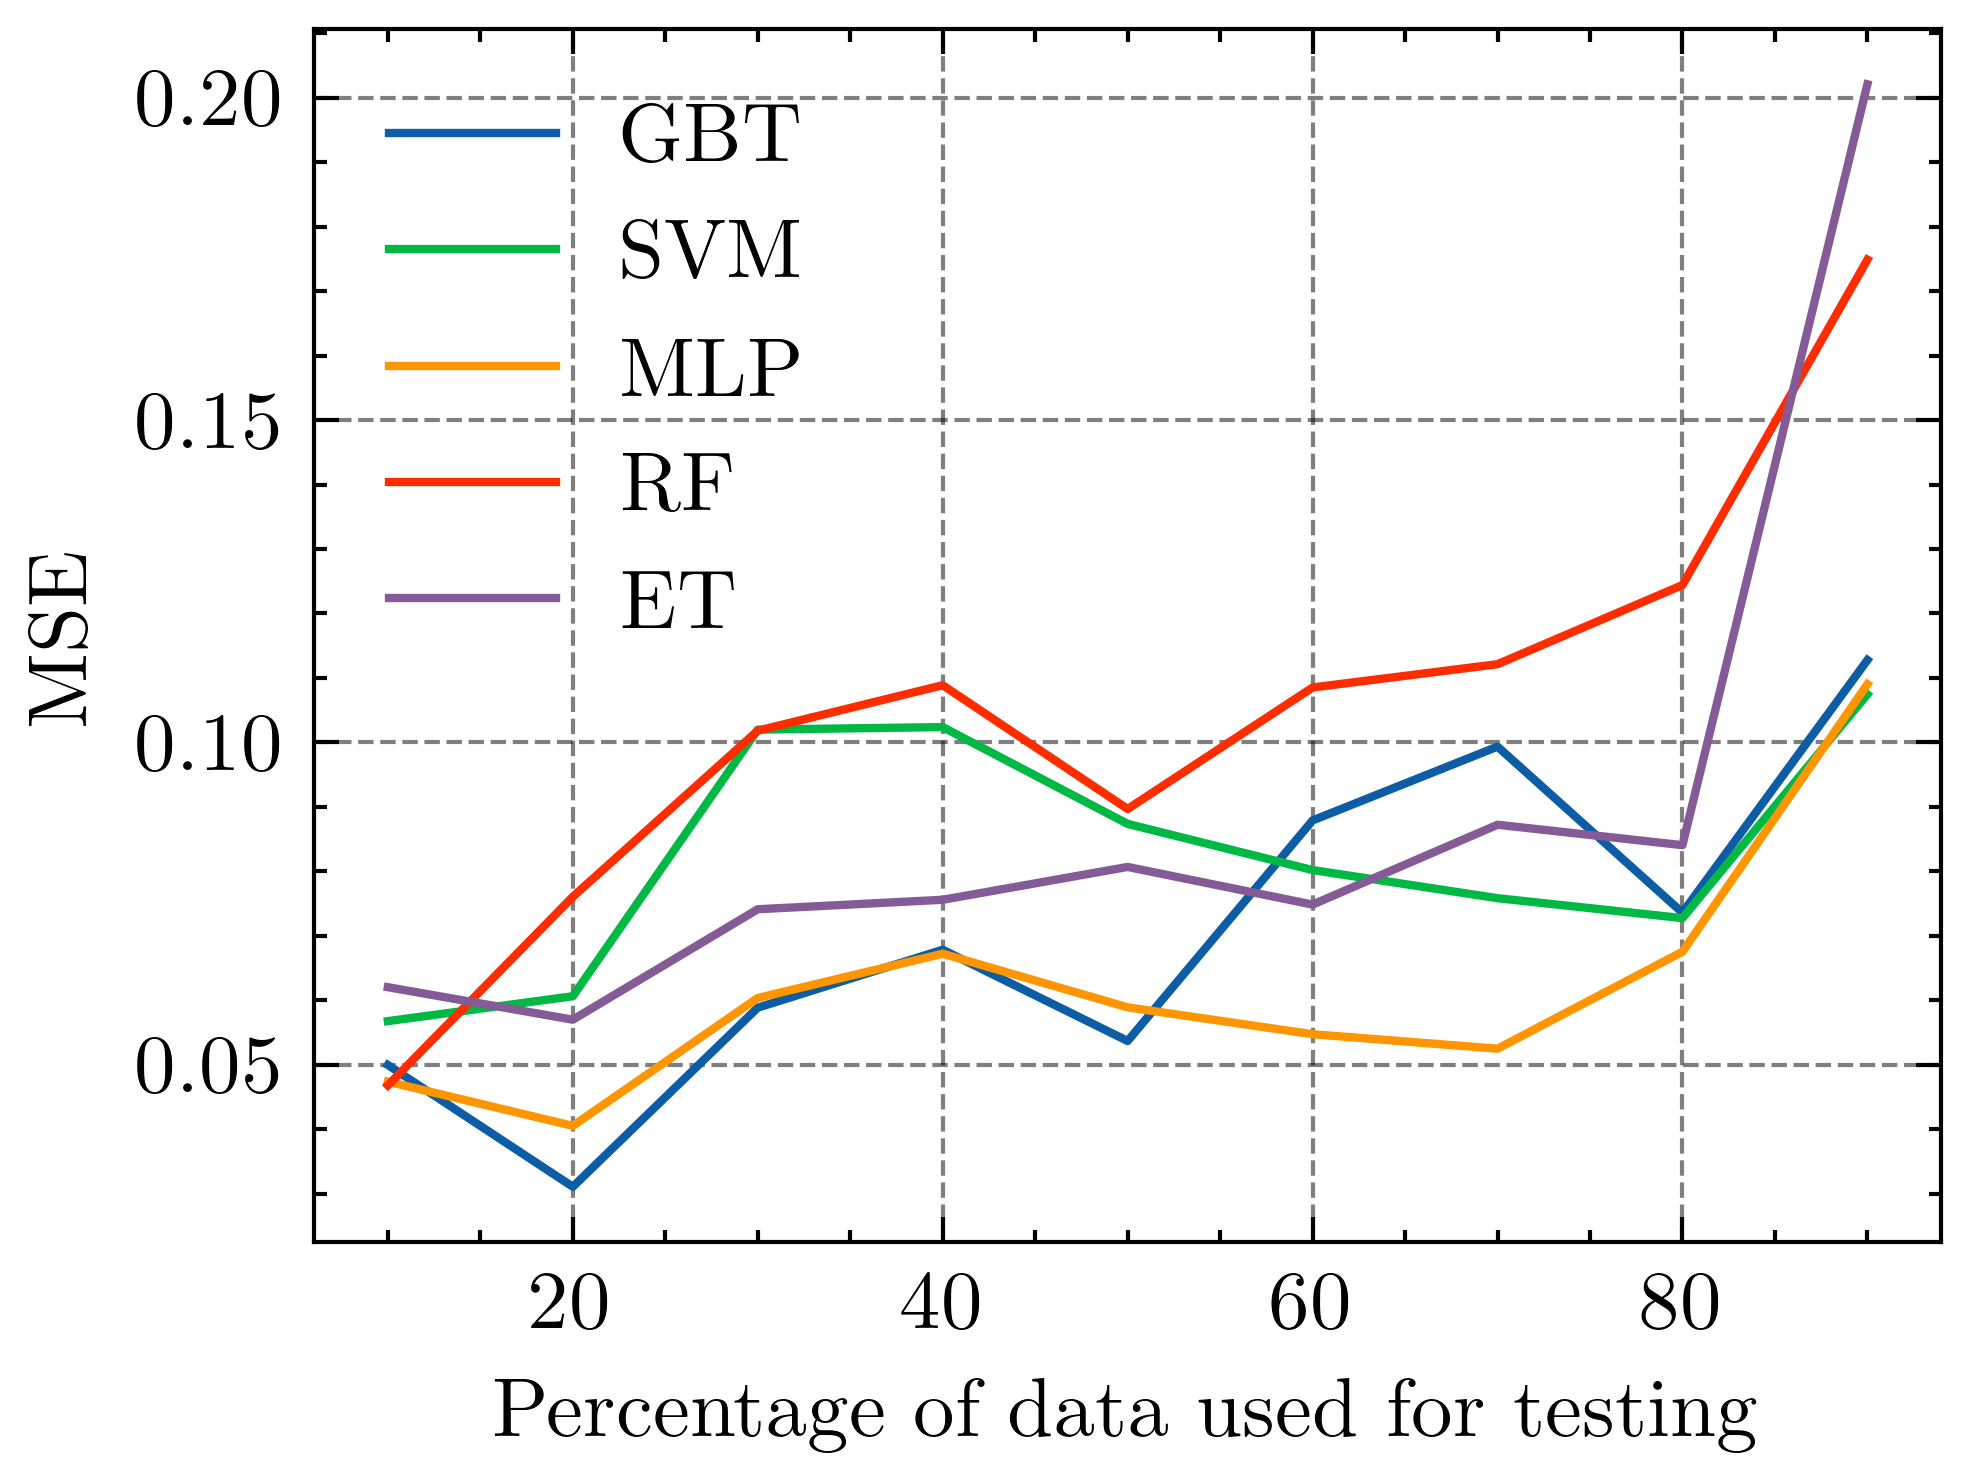
\includegraphics[width=\textwidth]{chap5/images/missing_values_plot}
            \caption{}
            \label{fig:first}
        \end{subfigure}
        \hfill
        \begin{subfigure}{0.4\textwidth}
            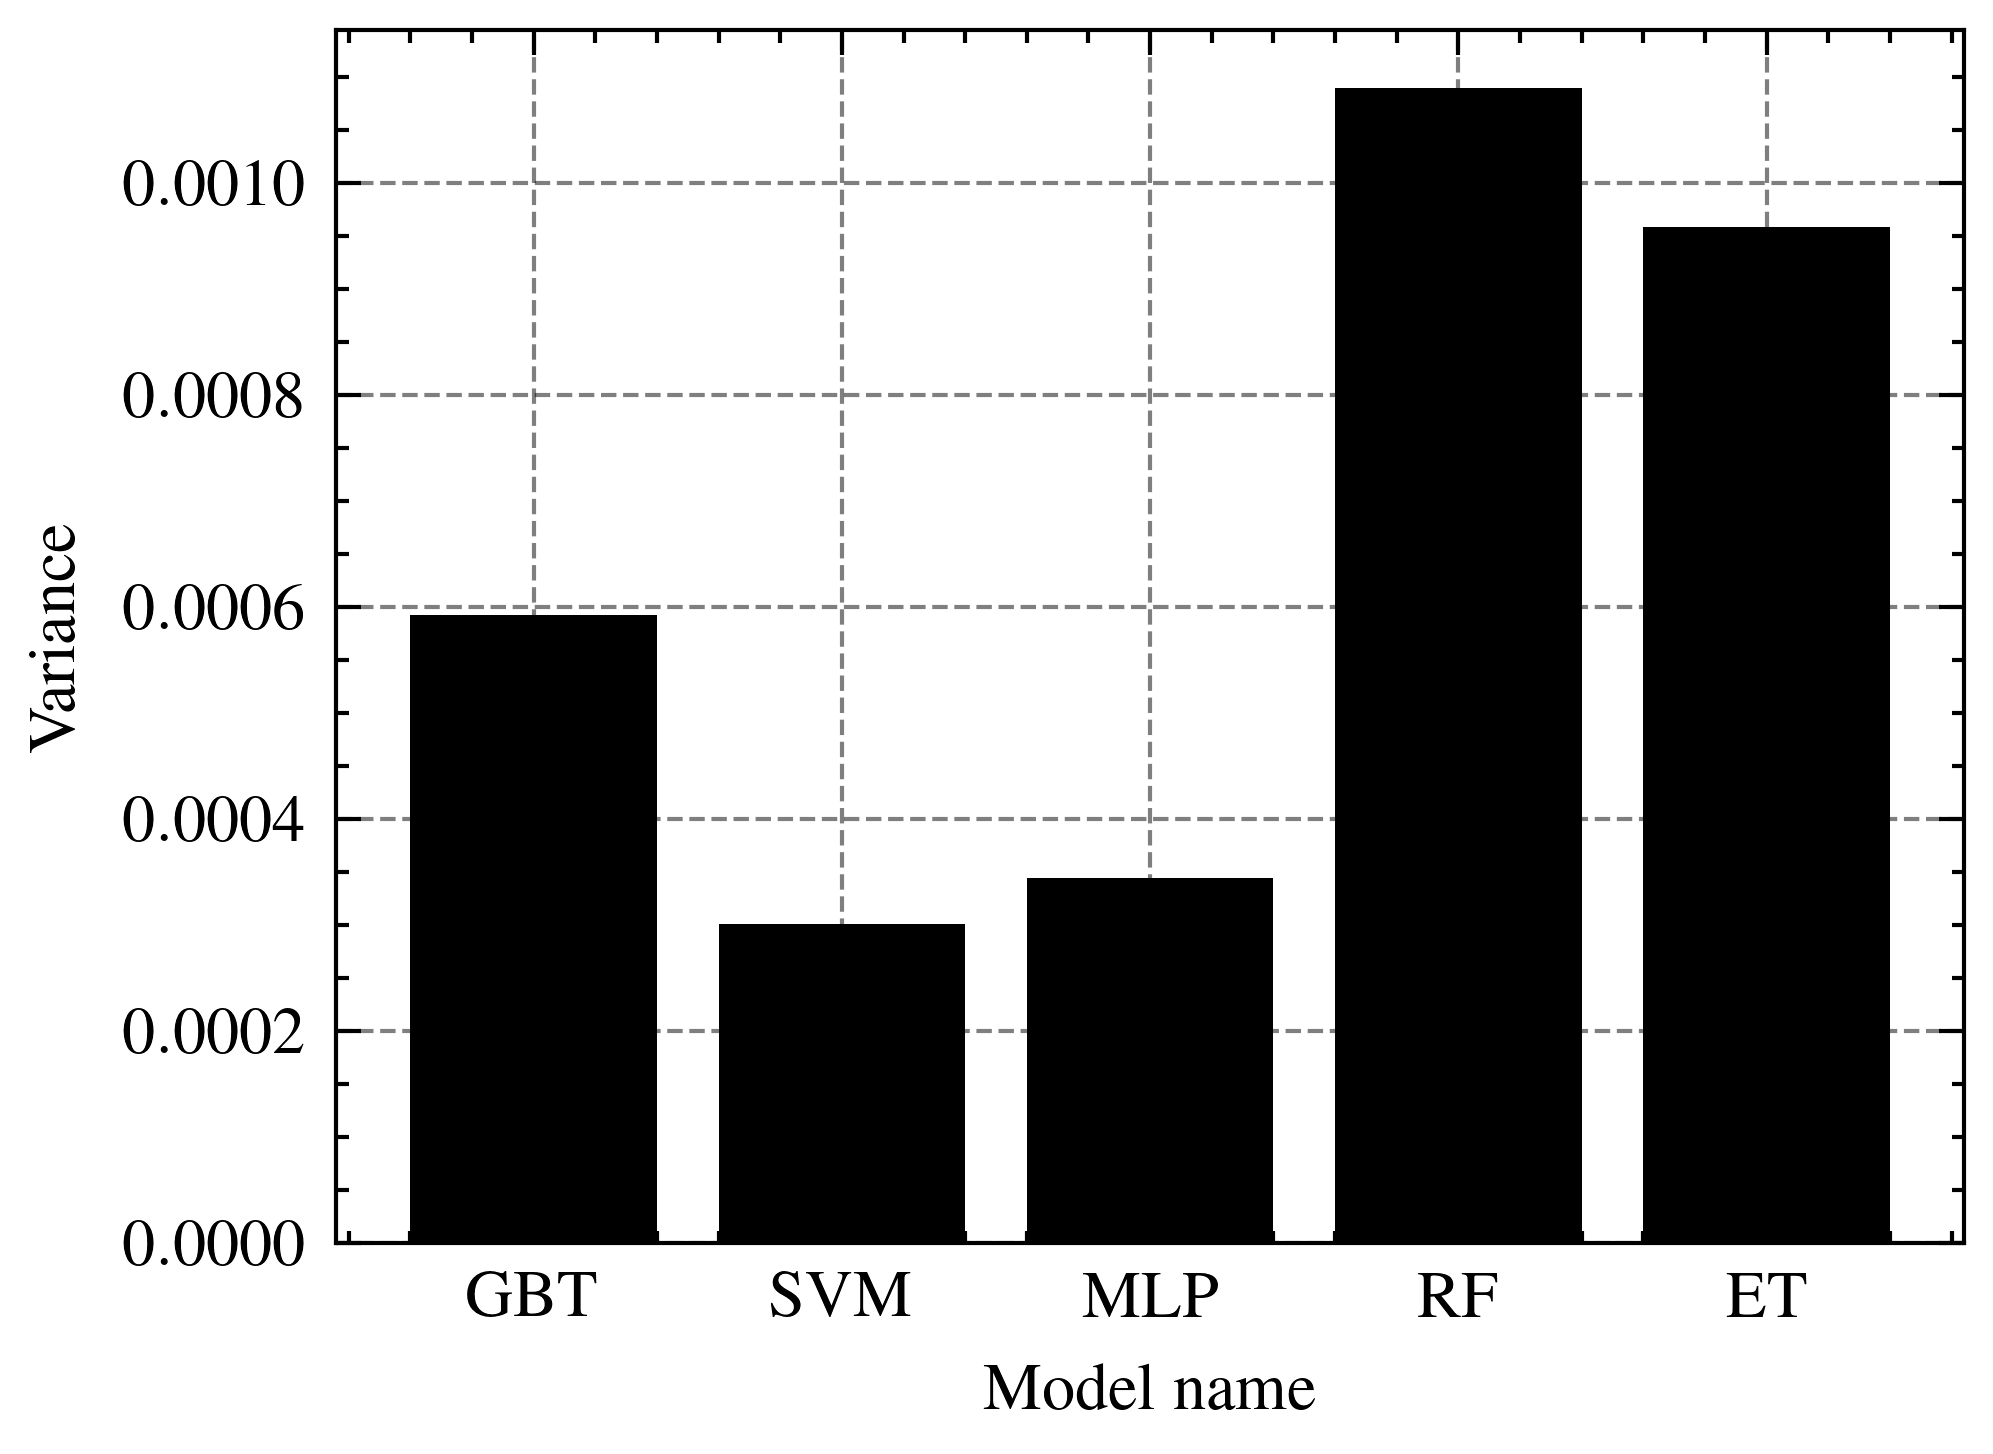
\includegraphics[width=\textwidth]{chap5/images/variance_missing_values}
            \caption{}
            \label{fig:second}
        \end{subfigure}
        \hfill
        \label{fig:results-missing-values}
    \end{tcolorbox}
    \caption{Figure (a) shows the comparison of performance on less data. Figure (b) shows the
    variance of the models when trained on less data.}
\end{figure}

%\begin{tcolorbox}[arc=0pt,boxrule=0.5pt]
%    \begin{equation}
%        \label{eq:average_loss}
%        \text{Loss of Accuracy} = \frac{1}{N} \sum_{i=1}^{N} |\text{RMSE}i -
%        \text{RMSE}{avg}|
%    \end{equation}
%\end{tcolorbox}

%Where \(N\) is the toal number of folds, \(i\) is the index of the current folds.
%
%It is worth noting that imputations of missing values can be used to mitigate
%the loss
%caused by missing data.
%However, this approach was not used in this thesis as the goal
%was to measure the robustness of the model to missing values specifically,
%rather than to
%artificially improve its performance through imputation techniques.

\subsection{Noise}\label{subsec:noise}
A common practise in \ac{ML} is to add noise to the training data to improve
the model's generalization abilities.
In the following section Gaussian Noise will be added to the data set to evaluate the robustness
of the model.

There is no standard approach to adding noise to the data.
In this thesis, the noise was added to the training data only.

To add the noise, \textit{numpy.random.normal} function was used, which
generate random numbers with a Gaussian distribution~\cite{scikit-learn}.
The mean and standard deviation of each feature were calculated based on the
original data, and the function was used to generate noisy values for each feature.

To study the model's reaction to increasing amounts of noise, the noise added
to the training data was gradually increased starting from 1\% to 50\%, which means that the
last iteration contains as many noisy as ``clean'' samples.

The difference between all \ac{RMSE} between iterations was defined as loss.
The total loss was calculated by averaging the difference of these values as shown in Equation~\ref{eq:noise}.

\begin{tcolorbox}[arc=0pt,boxrule=0.5pt]
    \begin{equation}
        \text{Average Loss} = \frac{1}{N} \sum_{i=1}^{N} |\text{RMSE}i -
        \text{RMSE}{avg}|\label
        {eq:noise}
    \end{equation}
\end{tcolorbox}

\begin{itemize}
    \item \textit{Does the calculation of the loss make sense?}
\end{itemize}

\subsection{Results}\label{subsec:results-robustness}

\begin{table}[H]
    \begin{tcolorbox}[arc=0pt,boxrule=0.5pt]
% \sisetup{group-minimum-digits = 4}
        \centering
        \begin{tabular}{llll}
            \toprule
            \thead{\textbf{Model Name}} & rs & {\thead{\textbf{Noise} \\ \unit{loa}}}
            \\
            \toprule
            \textbf{LR} & - & 0.070 & 0.251 \\
            .071 & 0.224 \\
            \hdashline
            \textbf{Random Forest} & x & 0.241 \\
            \hdashline
            \textbf{SVM} & - & 0.251 \\
            \hdashline
            \textbf{MLP} & - & 0.451 \\
            \bottomrule
        \end{tabular}
        \caption{Results of used machine learning models regarding the design
        principle robustness.}
        \label{tab:results_robustness}
    \end{tcolorbox}
\end{table}


\section{DP4: Stability}\label{sec:stability}
% Does the artifact generate repeatable results when trained on different data?
% Leave-one-out cross-validation stability 
Stability is defined as the ability of the model to generate repeatable
results when trained on different data~\cite[p. 16]{siebert2022construction}.

One appropriate way to measure the stability of a model is to use \ac{LOOCV},
which is a a form of \ac{CV} where one sample is used for validation and the remaining
data is used for training~\cite[p. 200--201]{gareth2013introduction}.
LOOCV is a technique where the observation set is divided into two parts, but instead of having
two subsets of comparable size, one sample is used for validation, while the rest form the
training set.

In order to evaluate the model the \ac{LOOCV} was repeated for all samples in
the dataset resulting in a total of \(n\) iterations.
The stability of the model was determined by calculating the average prediction error across all
iterations, using the equation provided in Equation~\ref{eq:loocv} which is taken from~\cite[p.
201]{gareth2013introduction}.

\begin{tcolorbox}[arc=0pt,boxrule=0.5pt]
    \begin{equation}
        CV_{(n)} = \frac{1}{n} \sum_{i=1}^{n} \text{MSE}_{i}\label{eq:loocv}
    \end{equation}
\end{tcolorbox}

The resulting \ac{MSE} is a poor estimate of the model's generalization error because only one
sample is used for validation~\cite[p. 201]{gareth2013introduction}, but it can be used to make a
statement about the stability.

The stability of the model can be evaluated by examining the standard derivation of the cross
validations scores.
A low standard derivation across all folds indicated that the model can generated consitent
results when trained on different datasets, suggesting are more sable model.

It is important to note that there are many different ways to measure the modelstability.
In this work LOOCV was chosen for three reasons.
%Another common approach is to use regular Cross-Validatoin, there are three reasons why LOOCV was
%chosen for this work.
Firstly, \ac{LOOCV} uses nearly all available data for training, while K-fold CV resevers a
portion o f the data for testing.
as the dataset used is relatfively small, it is an advantage to use all data for training.
Secondly, \ac{LOOCV} tends to have a lower bias due to the larger training set.
Lastly, multiple approaches have been tried to measure the model stabilty, and LOOCV delivered
he most stable and interpretable results.
The main drawback of the chose method is that it is computationally expensive as it required n
iterations.

Table~\ref{subsec:results-stability} shows the cross-validation score and the standard derivation
of each model. The focus relied more on the standard derivation, as it is a better indicator of
the stability of the model. As already mentioned the \ac{CV} score with using LOOCV is a poor
estimator.

---

\subsection{Results}\label{subsec:results-stability}

\begin{table}[H]
    \begin{tcolorbox}[arc=0pt,boxrule=0.5pt]
% \sisetup{group-minimum-digits = 4}
        \centering
        \begin{tabular}{ll}
            \toprule
            \thead{\textbf{Model Name}} & \thead{\textbf{std of CV scores (MSE)}}
            \\
            \toprule
            \textbf{Random Forest}          & 0.047 (0.891) \\
            \textbf{Random Forest}          & 0.200 (0.047) \\
            \hdashline
            \textbf{Gradient Boosting}      & 0.044 (0.922) \\
            \textbf{Gradient Boosting}      & 0.190 (0.039) \\
            \hdashline
            \textbf{Extra Trees}            & 0.46  (0.877)   \\
            \textbf{Extra Trees}            & 0.199 (0.053) \\
            \hdashline
            \textbf{Support Vector Machine} & 0.050 (0.853) \\
            \textbf{Support Vector Machine} & 0.266 (0.061) \\
            \hdashline
            \bottomrule
        \end{tabular}
    \end{tcolorbox}
    \caption{Results of the stability of the models.}
    \label{tab:results-stability}
\end{table}


\section{DP5: Resource utilization}\label{sec:resource-utilization}
% How much resources are required to train and run the model?
% Training time, runtime, storage space

To measure the resource utilization of the model, the following metrics are
used:

% From Copilot
\paragraph*{Training time}
Measured in seconds. Refers to the time it takes to train the model.
Training a model requires resources such as memory, CPU, and GPU, therefore
the longer it takes
to train a model, the more resources are required. According to resources
utilization a shorter
training time is desirable.

The training time is measured using the \texttt{time.time} function in python
. The function
returns the time in seconds since the epoch. The time is measured before and
after the model is
fitted. The difference between the two times is the training time.

\textbf{Inference time}
Measured in milliseconds. It refers to the time it takes to make a prediction
on data once it has
been trained.
It is an important measure not only for real-world application but also a
faster runtime uses
less resources and is therefore more efficient.

\textbf{Inference time}
Measured in milliseconds. Time it takes to make 100 predictions.
A model that takes longer to make predictions may be more complex than a
model that is able to
make predictions more quickly.
Measured using the \texttt{time.time} function in python. 100 valuees are
picked out of the teset
set and the time is measured before and after the prediciton is made.

\textbf{Memory space}
Measured in Mb.
It refers to the amount of memeory required to run the model.
The more storage space required to store the model, the more resources are
required to store it.
Therefore, a smaller storage space is desirable.
To measure the memory usage the \texttt{memory\_usage} function from the
\texttt{memory\_profiler}
package is used.


\begin{table}[H]
    \begin{tcolorbox}[arc=0pt,boxrule=0.5pt]
        \centering
        \begin{tabular}{lllll}
            \toprule
            \thead{\textbf{Model Name}} & {\thead{\textbf{rs}}} & {\thead{\textbf{
                Training
                time} \\
            \unit[]{ms}}}
            & {\thead{\textbf{Inference time} \\ \unit[]{ms}}} &
                {\thead{\textbf{Memory
            Usage} \\
            \unit{kb}}}
            \\
            \toprule
            \textbf{LR} & - & 3.14 & 0.982 & 269.887 \\
            \textbf{LR} & x & 3.558 & 1.157 & 269.887 \\
            \hdashline
            \textbf{DT} & - & 2.743 & 1.136 & 174.0 \\
            \textbf{DT} & - & 3.455 & 1.212 & 174.008 \\
            \hdashline
            \textbf{RF} & - & 25.205 & 2.886 & 173.219 \\
            \textbf{RF} & x & 26.821 & 2.269 & 173.266 \\
            \hdashline
            \textbf{ET} & - & 19.62 & 1.725 & 173.121 \\
            \textbf{ET} & x & 20.854 & 1.887 & 173.156 \\
            \hdashline
            \textbf{SVM} & - & 309.721 & 2.789 & 195.734 \\
            \textbf{SVM} & x & 310.018 & 2.793 & 195.746 \\
            \hdashline
            \textbf{MLP} & - & 19100.697 & 11.663 & 180.949 \\
            \textbf{MLP} & x & - & 19100.697 & 11.663 & 180.949 \\
            \bottomrule
        \end{tabular}
        \caption{Overview of the used machine learning models and their
        metrics.}
        \label{tab:resutls_resource_utilization}
    \end{tcolorbox}
\end{table}

As can be seen in Table~\ref{tab:resutls_resource_utilization}, the \ac{ET} is faster
than to th conventional \ac{RF}.
This expected since the most-time intensive part of the \ac{RF} is the splitting of the
nodes with determining the optimal threshold for each feature at each node
(see section~\ref{subsubsec:extra-trees}).
It has been observed, that this advantage is lost when the \texttt{n\_estimators}
parameter is set above 10.

The \ac{MLP} is the slowest model to train and to make predictions.
Most certainly this is because an \ac{MLP} typically has more parameters to learn and
has a deeper architecture, which means that it requires mor computations to train and
predict.
Also the training algorithm used is backpropagation, wich can be more computationally
intensive.
Also an \ac{MLP} trains all data at once and therefore cant parallelize the process.
It has to be noted, that tuning the hyperparameters is a time-consuming steps and the
chosen parameters might not be the optimal ones.


\section{DP6: Interpretability}\label{sec:interpretability}
% How well can the model be explained?
% Complexity measures (e.g., no. of parameters, depth)

% Sieber et al used
% %
%& Complexity measures (e.g., no. of parameters, depth) \\
% These metrics where changed
When following definitions of interpretability used in
section~\ref{sec:objectives-of-a-solution}, it is clear that it is not possible to
measure interpretability in a quantitative way, but other metohds can beu sed to measure the
interpretability of a model.
%Interpretable models allow the usage of global model-agnostic evaluation
%methods which will be used later in the evaluation of the models (see
%Section~\ref{sec:evaluation}).


According to~\cite{molnar2020interpretable} one way to make a model interpretable is to limit the
choice of algorithms to those that produce interpretable results.
Example of such algorithms include linear regression, logistic regression and decision
trees~\cite[p. 35]{molnar2020interpretable}.

%\cite{molnar2020interpretable} defines three properties of interpretable models: linearity,
%monotonicity and interactions.
%A linear model expresses the relationship between features and the target outcome aa a linerar
%equation~\cite[]{molnar2020interpretable}.
%Monotonocitiy constraints ensure that there is a consistent relationship between a feature and
%the target outcome across the etnire renage of the feature. This can make it easier to understand
%the relationship.
%Some models automatically include interactions between features to improve prediciotn, while
%other require the manual creation of interaction features. However, inlcuding too many or complex
%interactions can make the model more difficult to interpret~\cite{molnar2020interpretable}.

%In the model selection for this thesis the focuses mostly on interpretable models,
%as they are easier to understand and explain, therefore mostly models are chosen which fulfill
%all three properties.
%
%Later in the thesis, the interpretability of the models is used to explain
%the results.

\subsection{Interpretable Models}\label{subsec:interpretable-models}
Linear Regression and Decision Trees are considered as interpretable models and offer good
model-specific explanations by default~\cite{molnar2020interpretable}.
As mentioned in section~\ref{sec:dp1:-correctness}, both algorithms perform not good enough
to be considered as a solution for the problem.
Therefore the focus is on model agnostic methods to explain the predictions of the models.

Also~\cite{molnar2020interpretable} differentiates between global and local
interpretability. Global
interpretability refers to the ability to understand the overall behavior of
the model, while local interpretability refers to the ability to understand the behavior of the
model for a specific instance.

As seen in the previous sections six different models were trained.
It does not make sense to apply model-agnostic method on all six models, it makes more sense to
apply the methods on the best performing models.
Therefore in a first step in the section~\ref{subsec:overall-comparison-model-performance} the
best performing models
are identified and in a second step model-agnostic interpretability methods are applied to
explain the predictions of the models.

For the current dataset, the V/t ratios range from 3.3 to 100. The highest ratio can be achieved
by bending a 0.5 mm thin metal sheet using a 50 mm wide die opening, while the lowest ratio is
achieved by bending a 3 mm thick sheet on the same die opening.

Recommended V/t ratios in industrial practices are between 6 and 10~\cite[p.7]{
    cruz_applicationmachinelearning_2021}.
Bending operations performed outside of this range of recommended ratios may result in
high spring back.

The selected representative instances for the local methods are from one of three cases:
\begin{itemize}
    \item Case A includes instances with V/t ratios below the recommended range.
    \item Case B includes instances within the recommended range of V/t ratios.
    \item Case C includes instances with V/t ratios above the recommended range.
\end{itemize}

Chosen instances from each case are shown in Table~\ref{tab:representative-instances}.

\begin{table}[H]
    \begin{tcolorbox}[arc=0pt,boxrule=0.5pt]
        \centering
        \begin{tabular}{lllll}
            \toprule
            \textbf{Case} & \textbf{\(V\) } & \textbf{\(t\)} & \textbf{\(y_p\)} & \textbf{V/t} \\
            \toprule
%            A             & 10              & 2.0            & ?                & 5            \\
            A             & 20              & 3              & ?                & 6.66         \\
            \hdashline
            \hdashline
            B             & 30              & 2              & ?                & 15           \\
            B             & 20              & 1              & ?                & 20           \\
%            B             & 30              & 1.5            & ?                & 20           \\
            \hdashline
            C             & 50              & 1              & ?                & 50           \\
            C             & 50              & 0.5            & ?                & 100          \\
            \bottomrule
        \end{tabular}
    \end{tcolorbox}
    \caption{Representative instances for the local methods.}
    \label{tab:representative-instances}
\end{table}

\subsection{Comparison of the Models}\label{subsec:overall-comparison-model-performance}
This section will showcase the outcomes generated by the trained models in more detail and
will also discuss the results in relation to the research questions.
This is done in this section to find out the best perfoming models.
These models will be researched in more detail later with the help of model-agnostic
methods to explain the predictions of the models.

In order to evaluate the model's performance without bias, each test case where removed
from the training data set so that the model has not seen the test case before.
This results in a small but notable performance decrease in the test cases, but makes sure that the
results are not biased.

For the interpretation of the next picutres it is relevant to nkow that the target values
repesent the man of all values.
The quality the dataset is but not perfect, and it is possible that there are some outliers in the
dataset.

Figure~\ref{fig:performance-case-a} shows show two chosen test cases for case A with a
V/t-ratio of 20 (\ref{fig:performance-20-1} and 6.6 (\ref{fig:performance-20-3}.

Case~\ref{fig:performance-20-1} with a V/t-ratio of 20 demonstrates the models'
ability to predict the spring with high accuracy.
However, the performance decreases in case b)\ref{fig:performance-20-3} with a V/t-ratio
of 6.6, particularly when predicting the spring backs.
It is likely that there is a measurement error at V = 7.5 in case
b)~\ref{fig:performance-20-3}, causing some models to potentially predict the correct
spring back.

\begin{figure}[H]
    \begin{tcolorbox}[arc=0pt,boxrule=0.5pt]
        \begin{subfigure}{0.5\textwidth}
            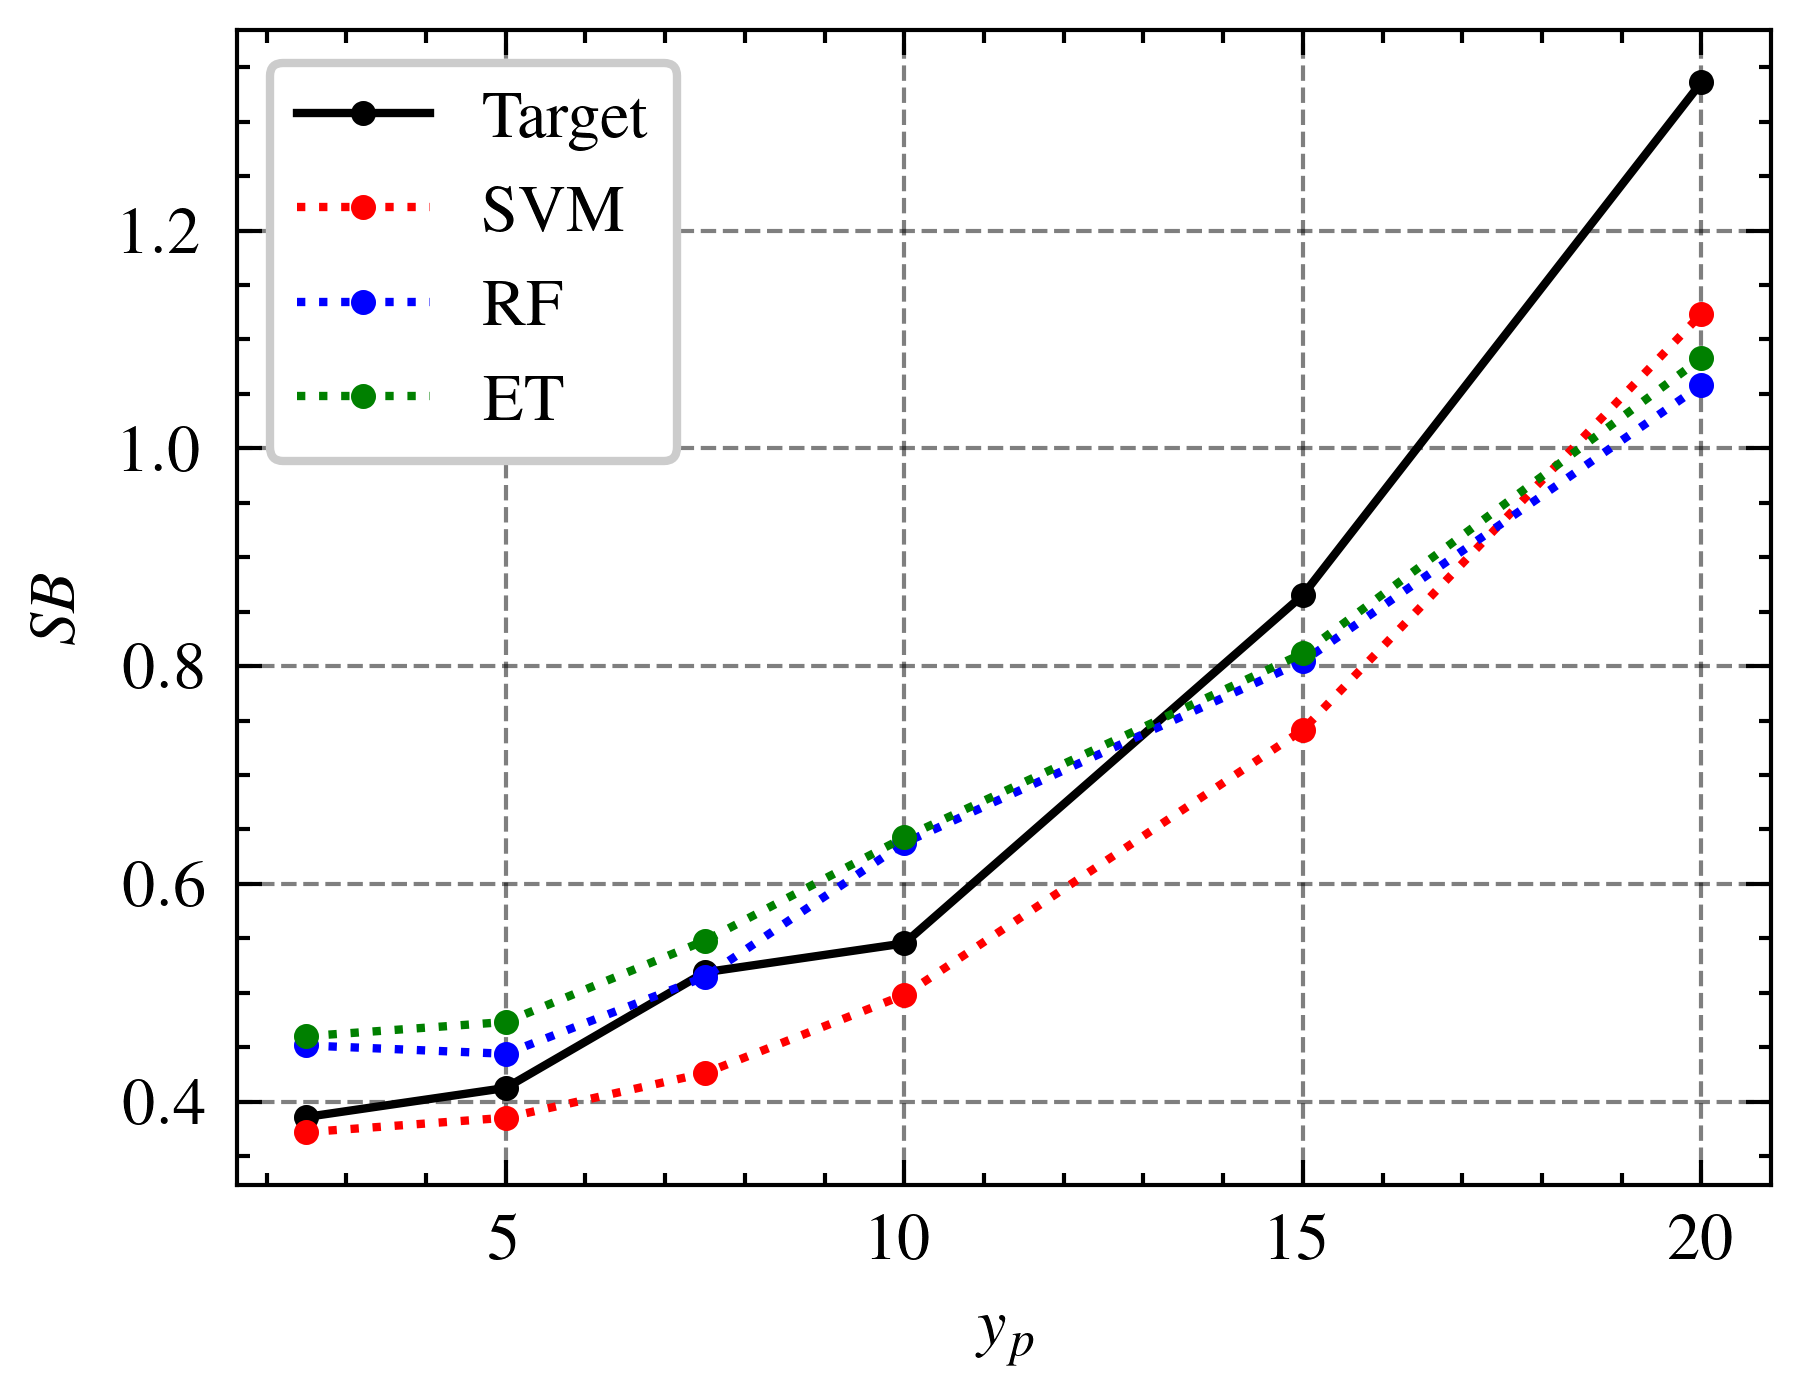
\includegraphics[width=\textwidth]{chap5/images/performance_20_3}
            \caption{V: 20, t: 1}
            \label{fig:performance-20-3-1}
        \end{subfigure}
        \hfill
        \begin{subfigure}{0.5\textwidth}
            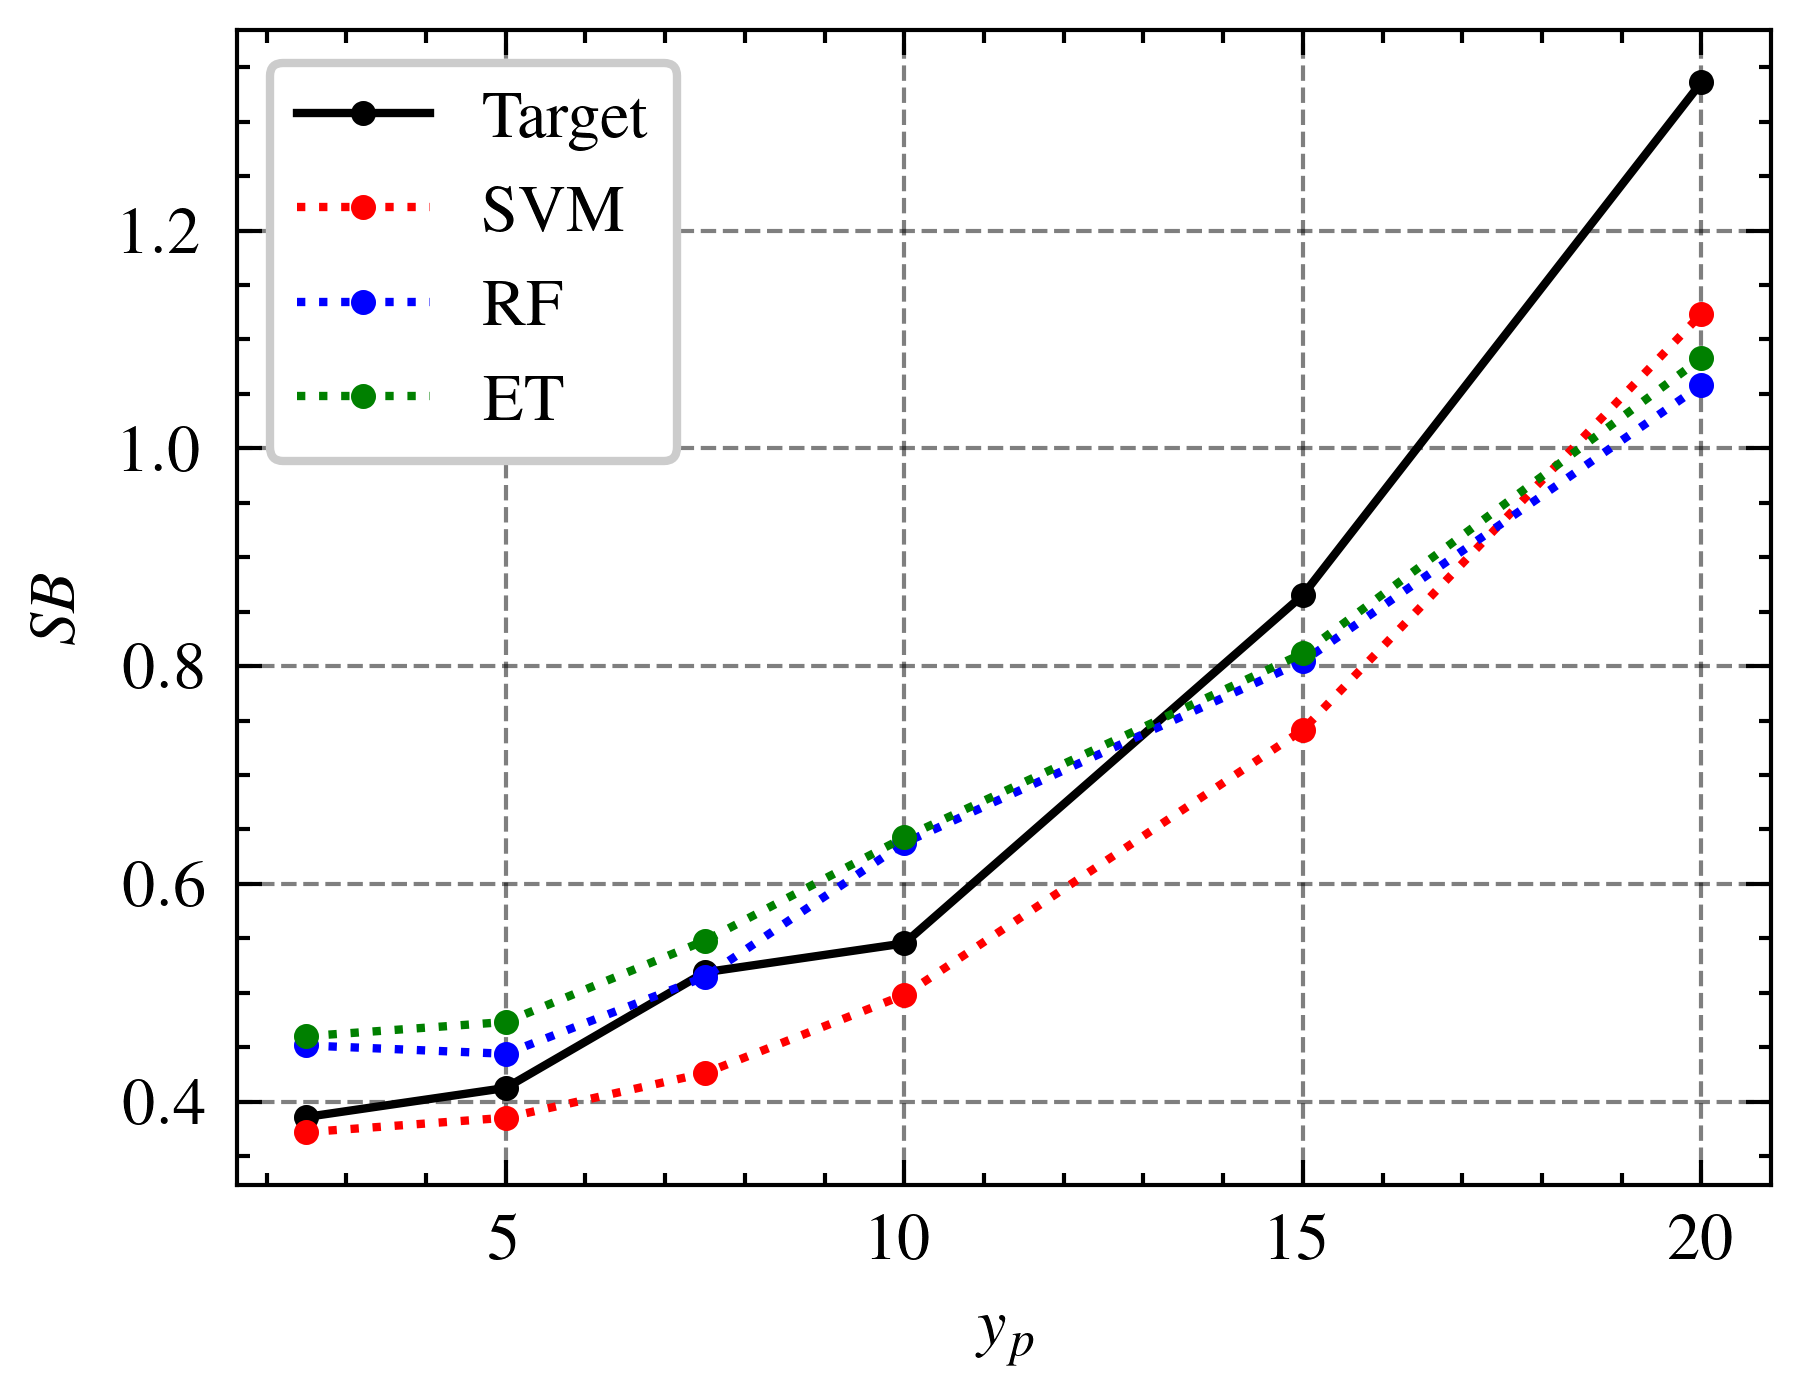
\includegraphics[width=\textwidth]{chap5/images/performance_20_3}
            \caption{V: 20, t: 3}
            \label{fig:performance-20-3-2}
        \end{subfigure}
    \end{tcolorbox}
    \caption{Performance plots for case A}
    \label{fig:performance-case-a}
\end{figure}


Figure~\ref{fig:performance-case-b} displays two selected test series for case B, which indicates
that the V/t ratios fall within the recommended range. These test series produced the best
results compared to cases A and C.

As depicted in figure~\ref{fig:performance-20-1}, both models accurately predicted the spring
back with high precision. The \ac{RF}, \ac{SVM}, and \ac{MLP} models demonstrated similar
performance and produced usable results. Similar findings were observed for figure~\ref{fig
:performance-30_2.0}, where the V/t ratio was different. In this case, the \ac{MLP} model
performed well for \(y_p\) values of 5 and 10, but became inaccurate for higher values. On the
other hand, the \ac{SLP} model consistently produced better results, while the \ac{ET} model
still struggled to perform well.

Overall, it is challenging to identify a clear favorite model based on the performance of the
models in these test series.
While some models performed better than others for specific variables or scenarios, the
differences were not significant enough to identify a clear winner.
Therefore, selecting an appropriate model will be decided by the other two cases A and C.

\begin{figure}[H]
    \begin{tcolorbox}[arc=0pt,boxrule=0.5pt]
        \begin{subfigure}{0.5\textwidth}
            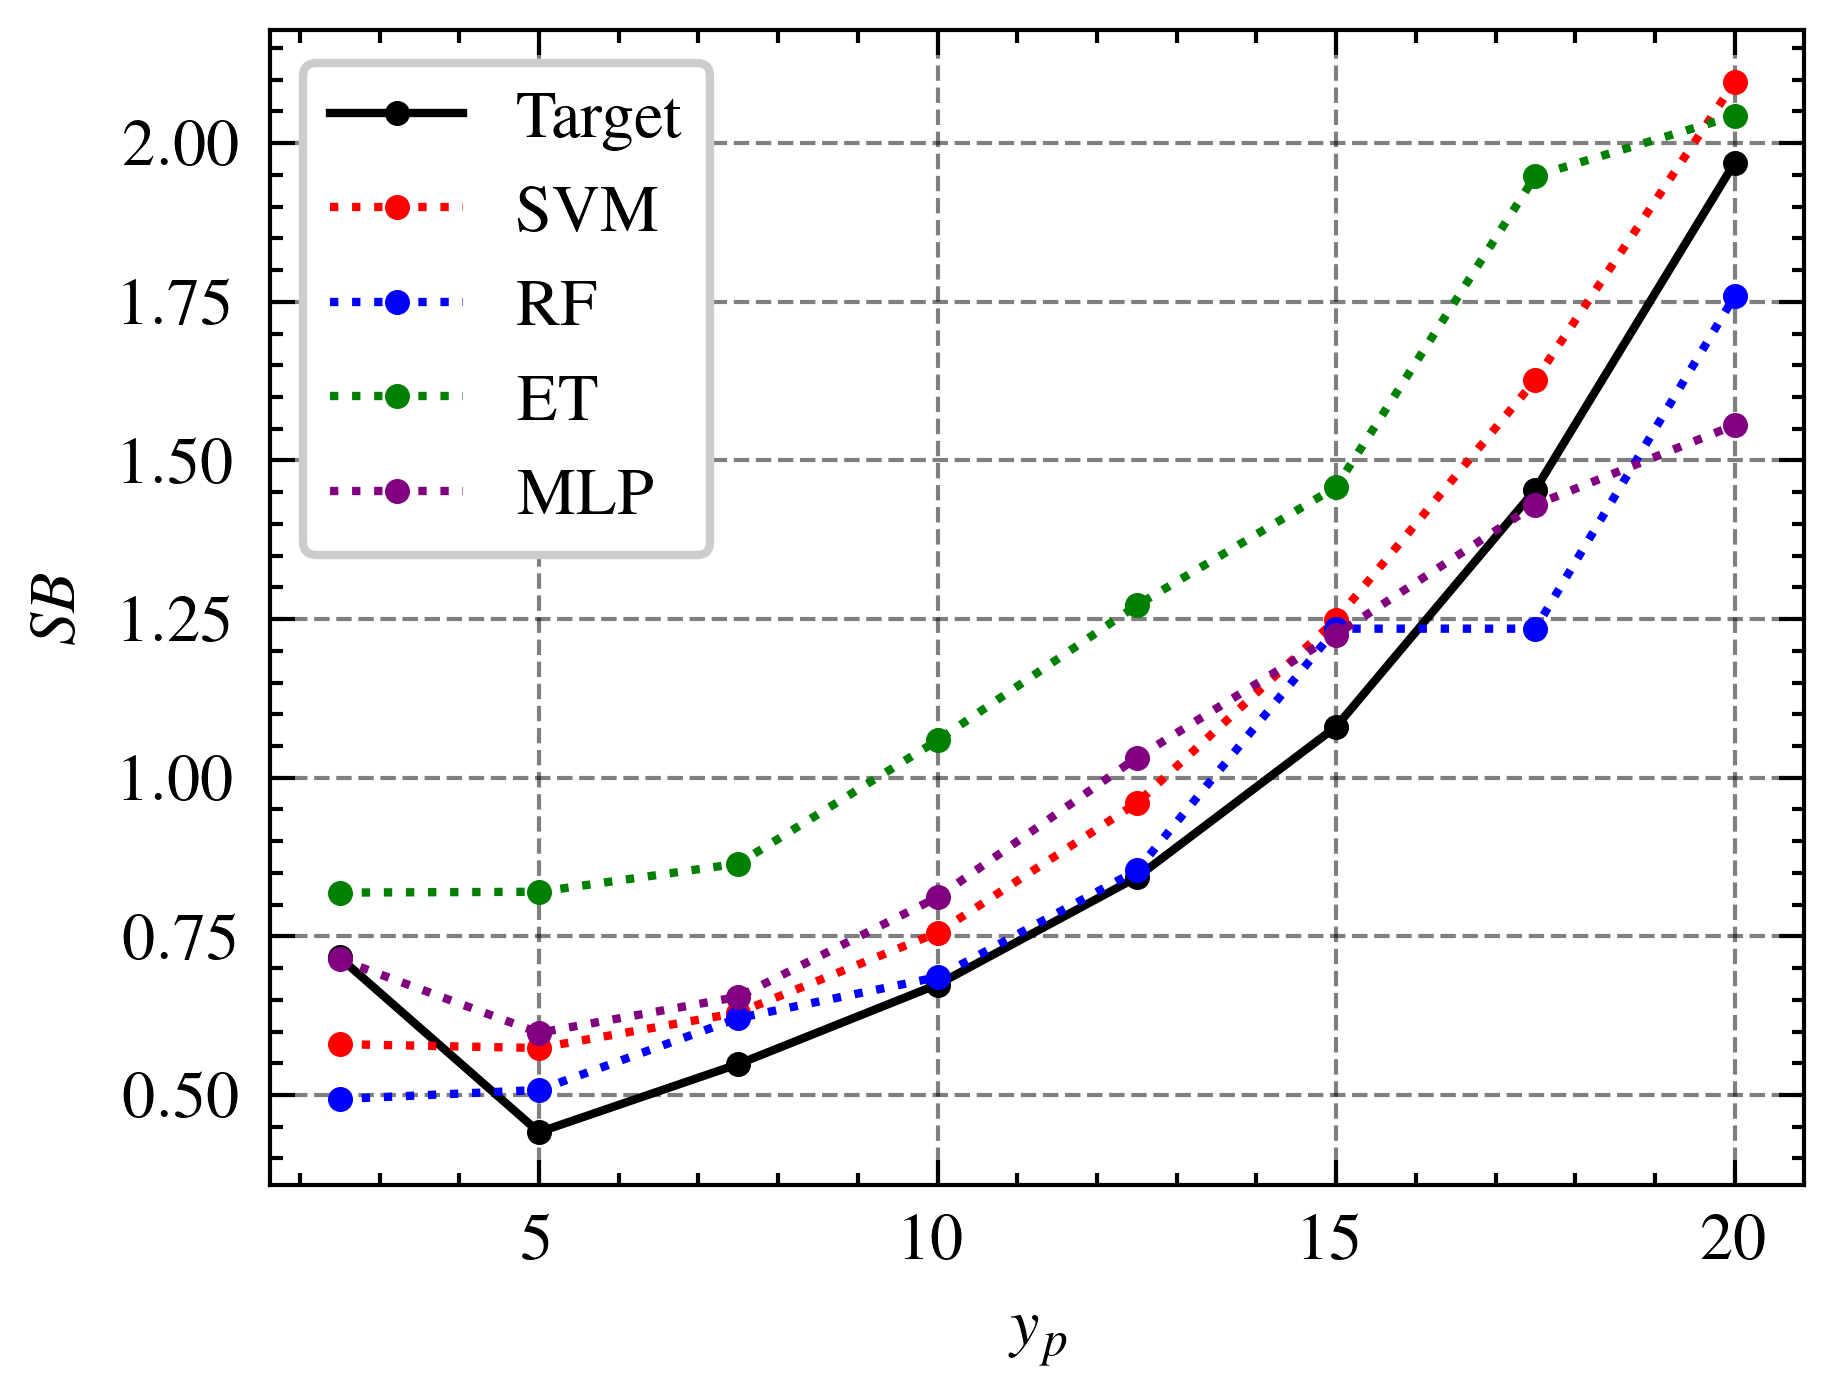
\includegraphics[width=\textwidth]{chap5/images/performance_20_1}
            \caption{V: 20, t: 1}
            \label{fig:performance-20-1}
        \end{subfigure}
        \hfill
        \begin{subfigure}{0.5\textwidth}
            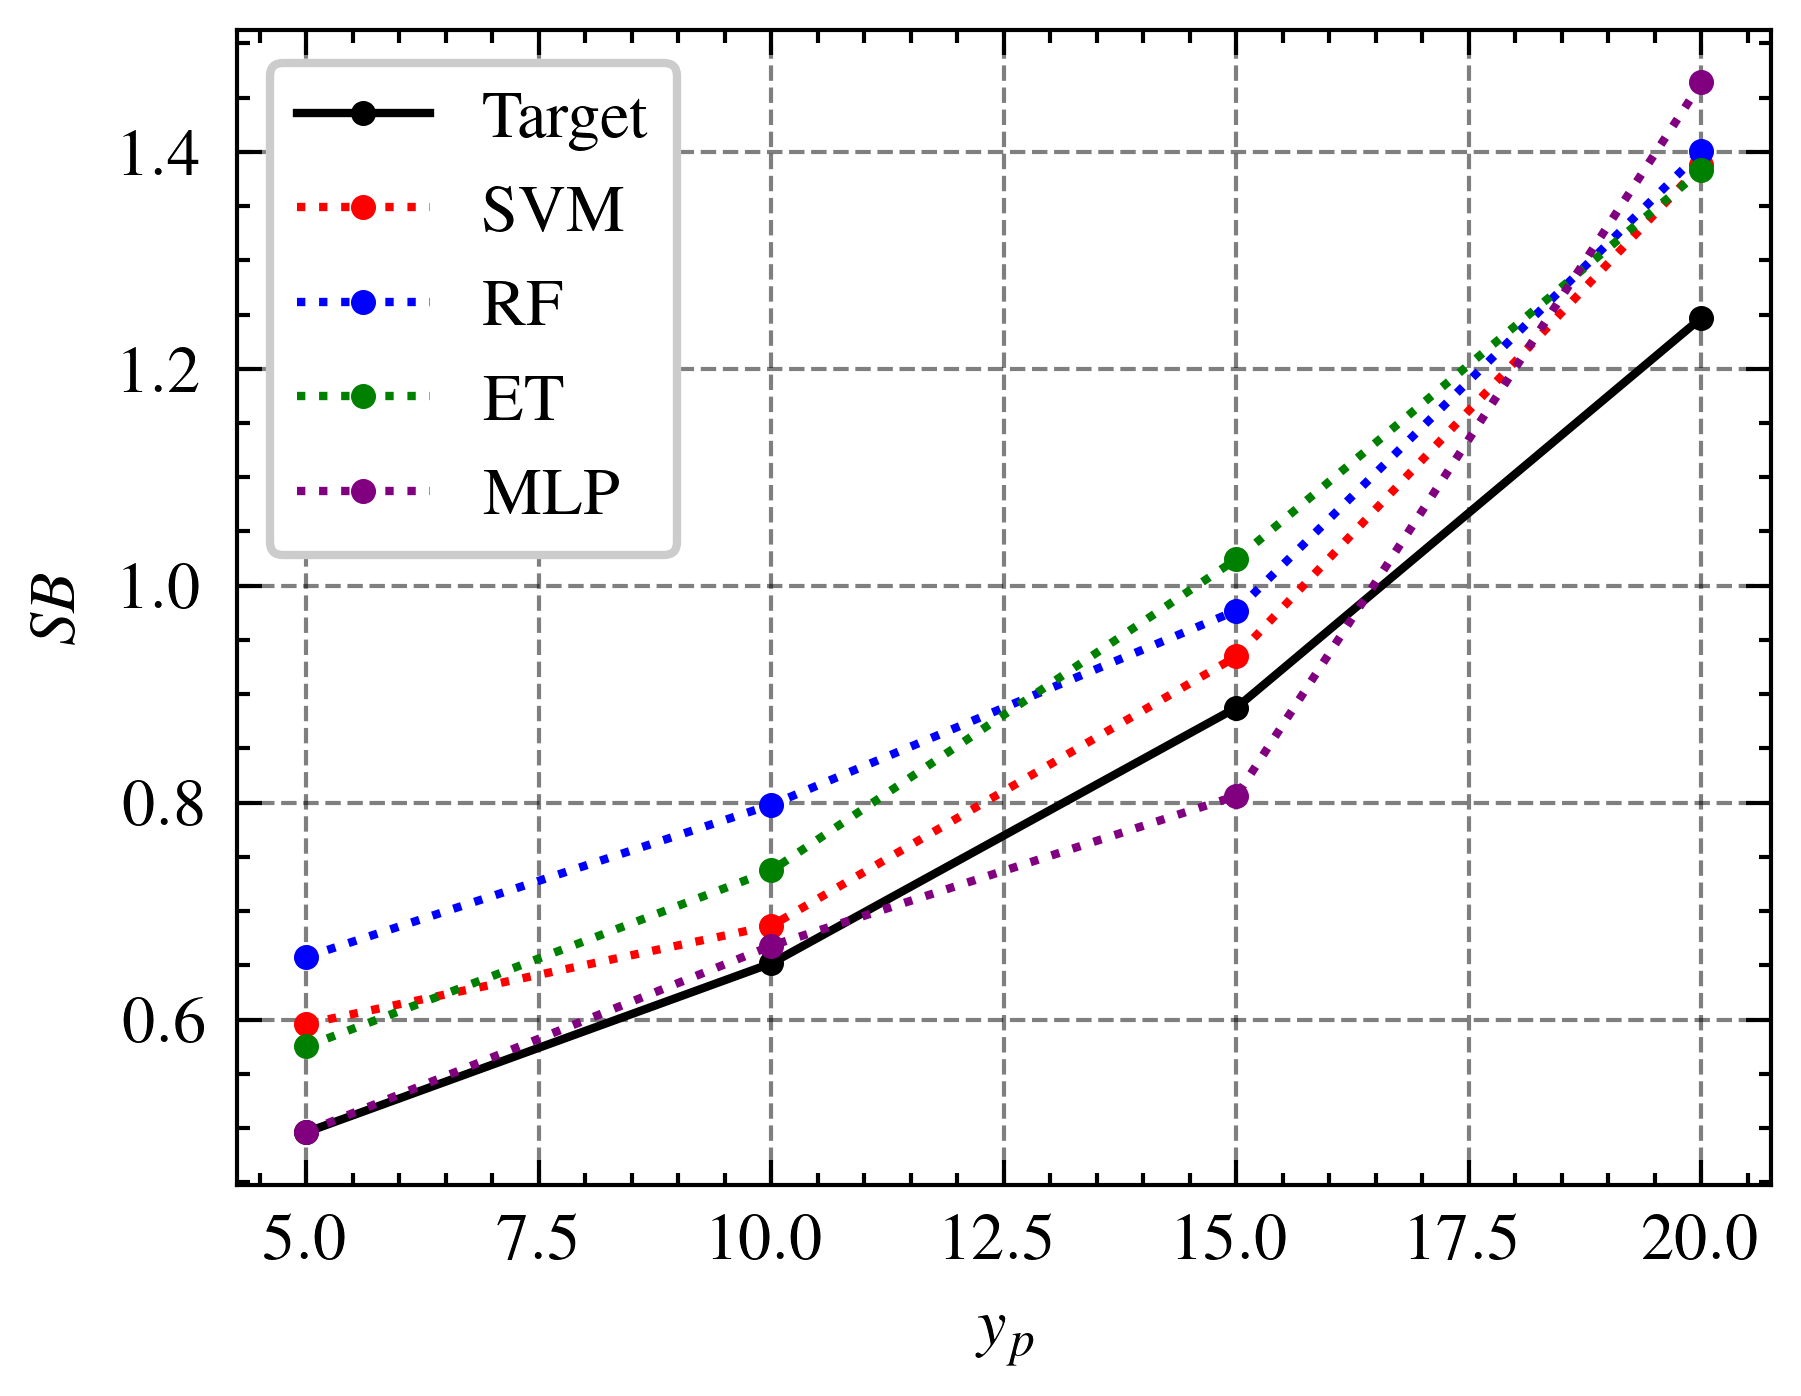
\includegraphics[width=\textwidth]{chap5/images/performance_30_2}
            \caption{V: 30, t: 2}
            \label{fig:performance-30_2.0}
        \end{subfigure}
    \end{tcolorbox}
    \caption{Performance plots for case B}
    \label{fig:performance-case-b}
\end{figure}

Case C is the most challenging case, as the V/t ratios are not within the recommended range.
Figure~\ref{fig:performance-case-c} shows the performance of the models for two test series
with V/t ratios of 50 and 100.

The results shown in figure~\ref{fig:performance-50_0.5} are clear.
The results are unusable, as the models are not able to predict the spring back.
In figure ~\ref{fig:performance-50_1} the results look better, the \ac{RF} and \ac{SVM} model
seem to be the most consistent models?

\begin{figure}[H]
    \begin{tcolorbox}[arc=0pt,boxrule=0.5pt]
        \begin{subfigure}{0.5\textwidth}
            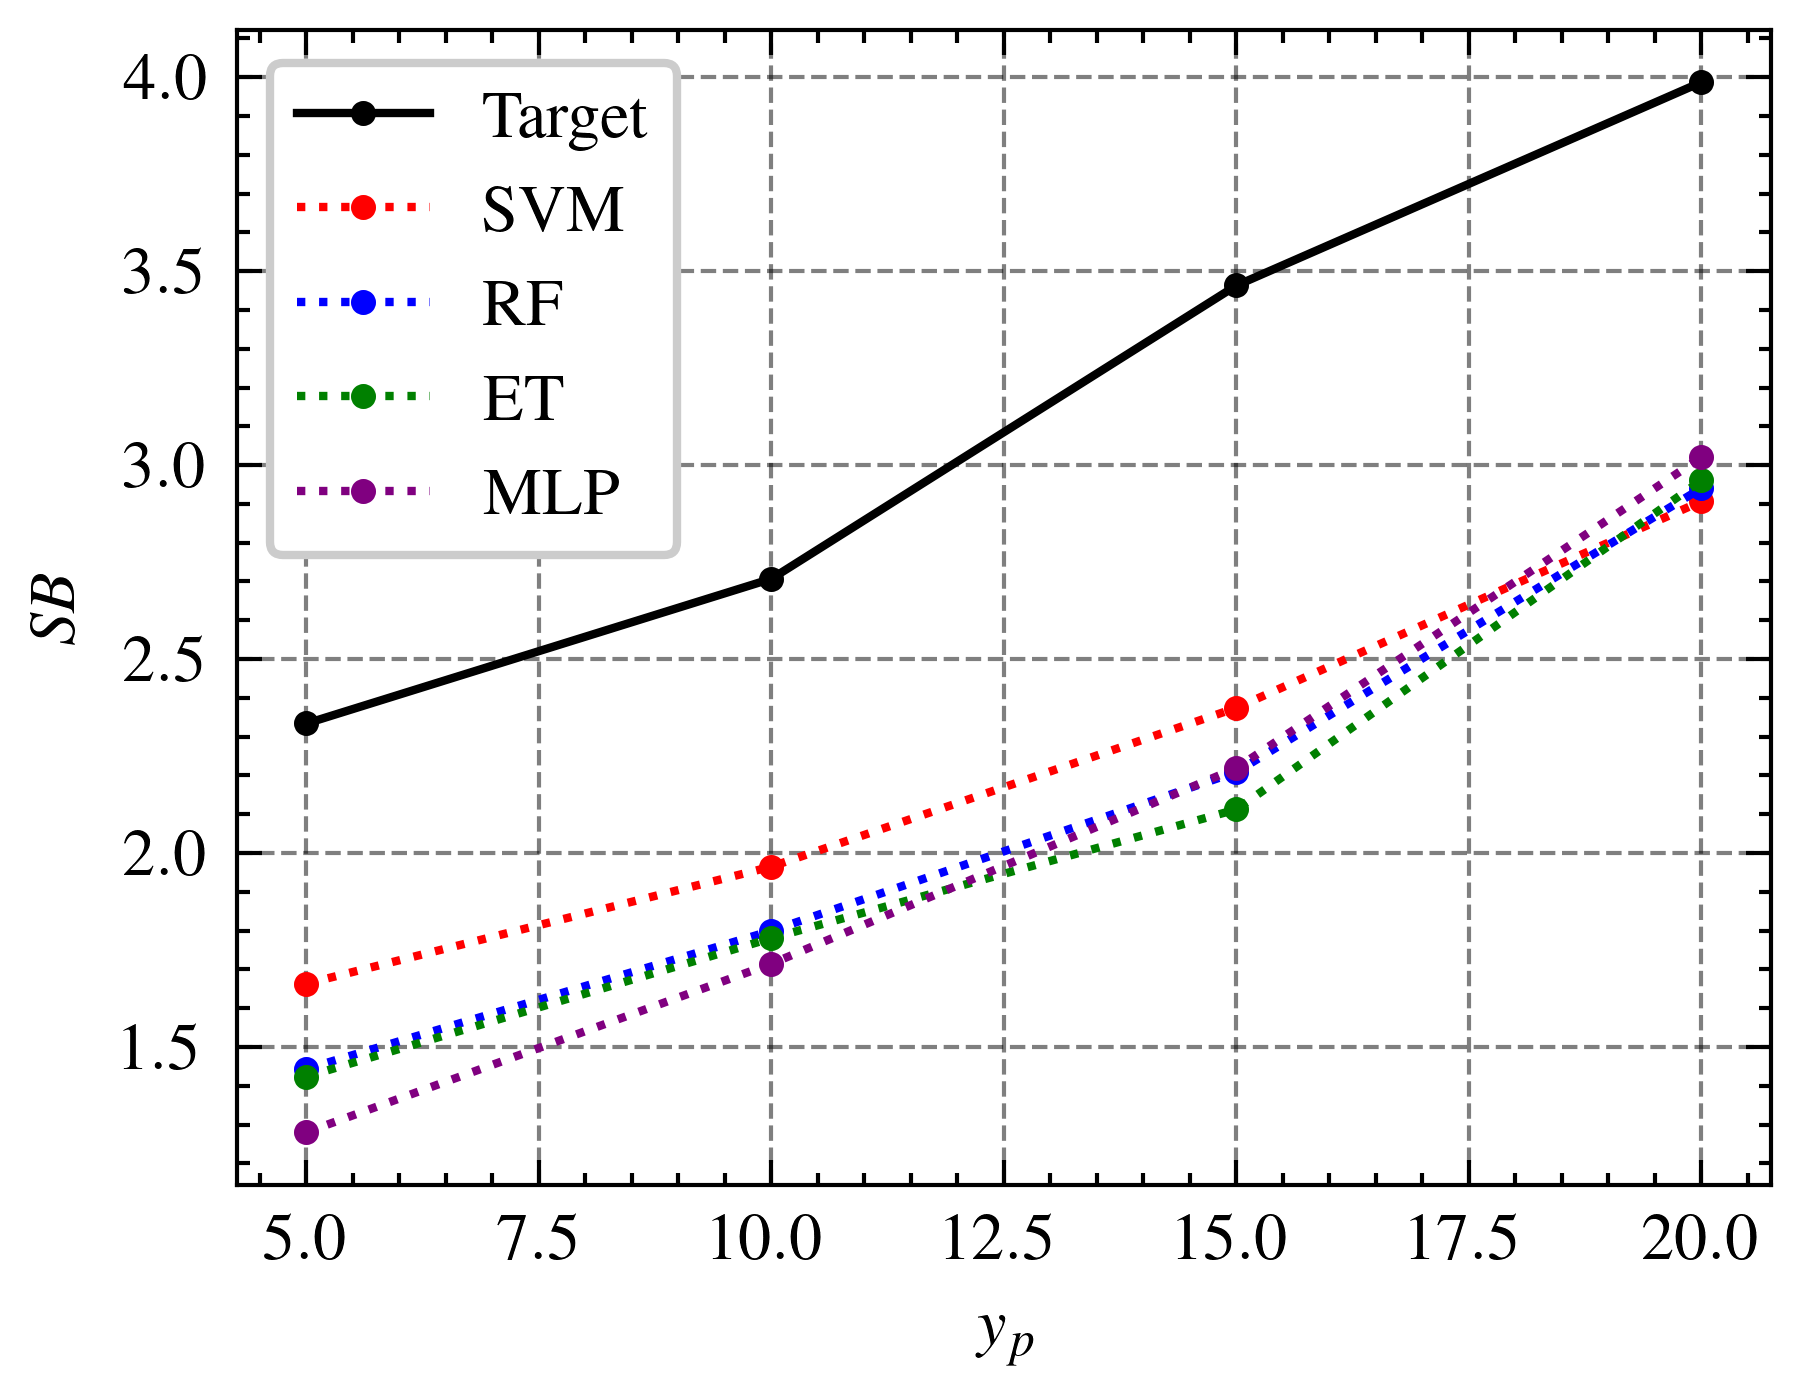
\includegraphics[width=\textwidth]{chap5/images/performance_50_0.5}
            \caption{V: 50, t: 0.5}
            \label{fig:performance-50_0.5}
        \end{subfigure}
        \hfill
        \begin{subfigure}{0.5\textwidth}
            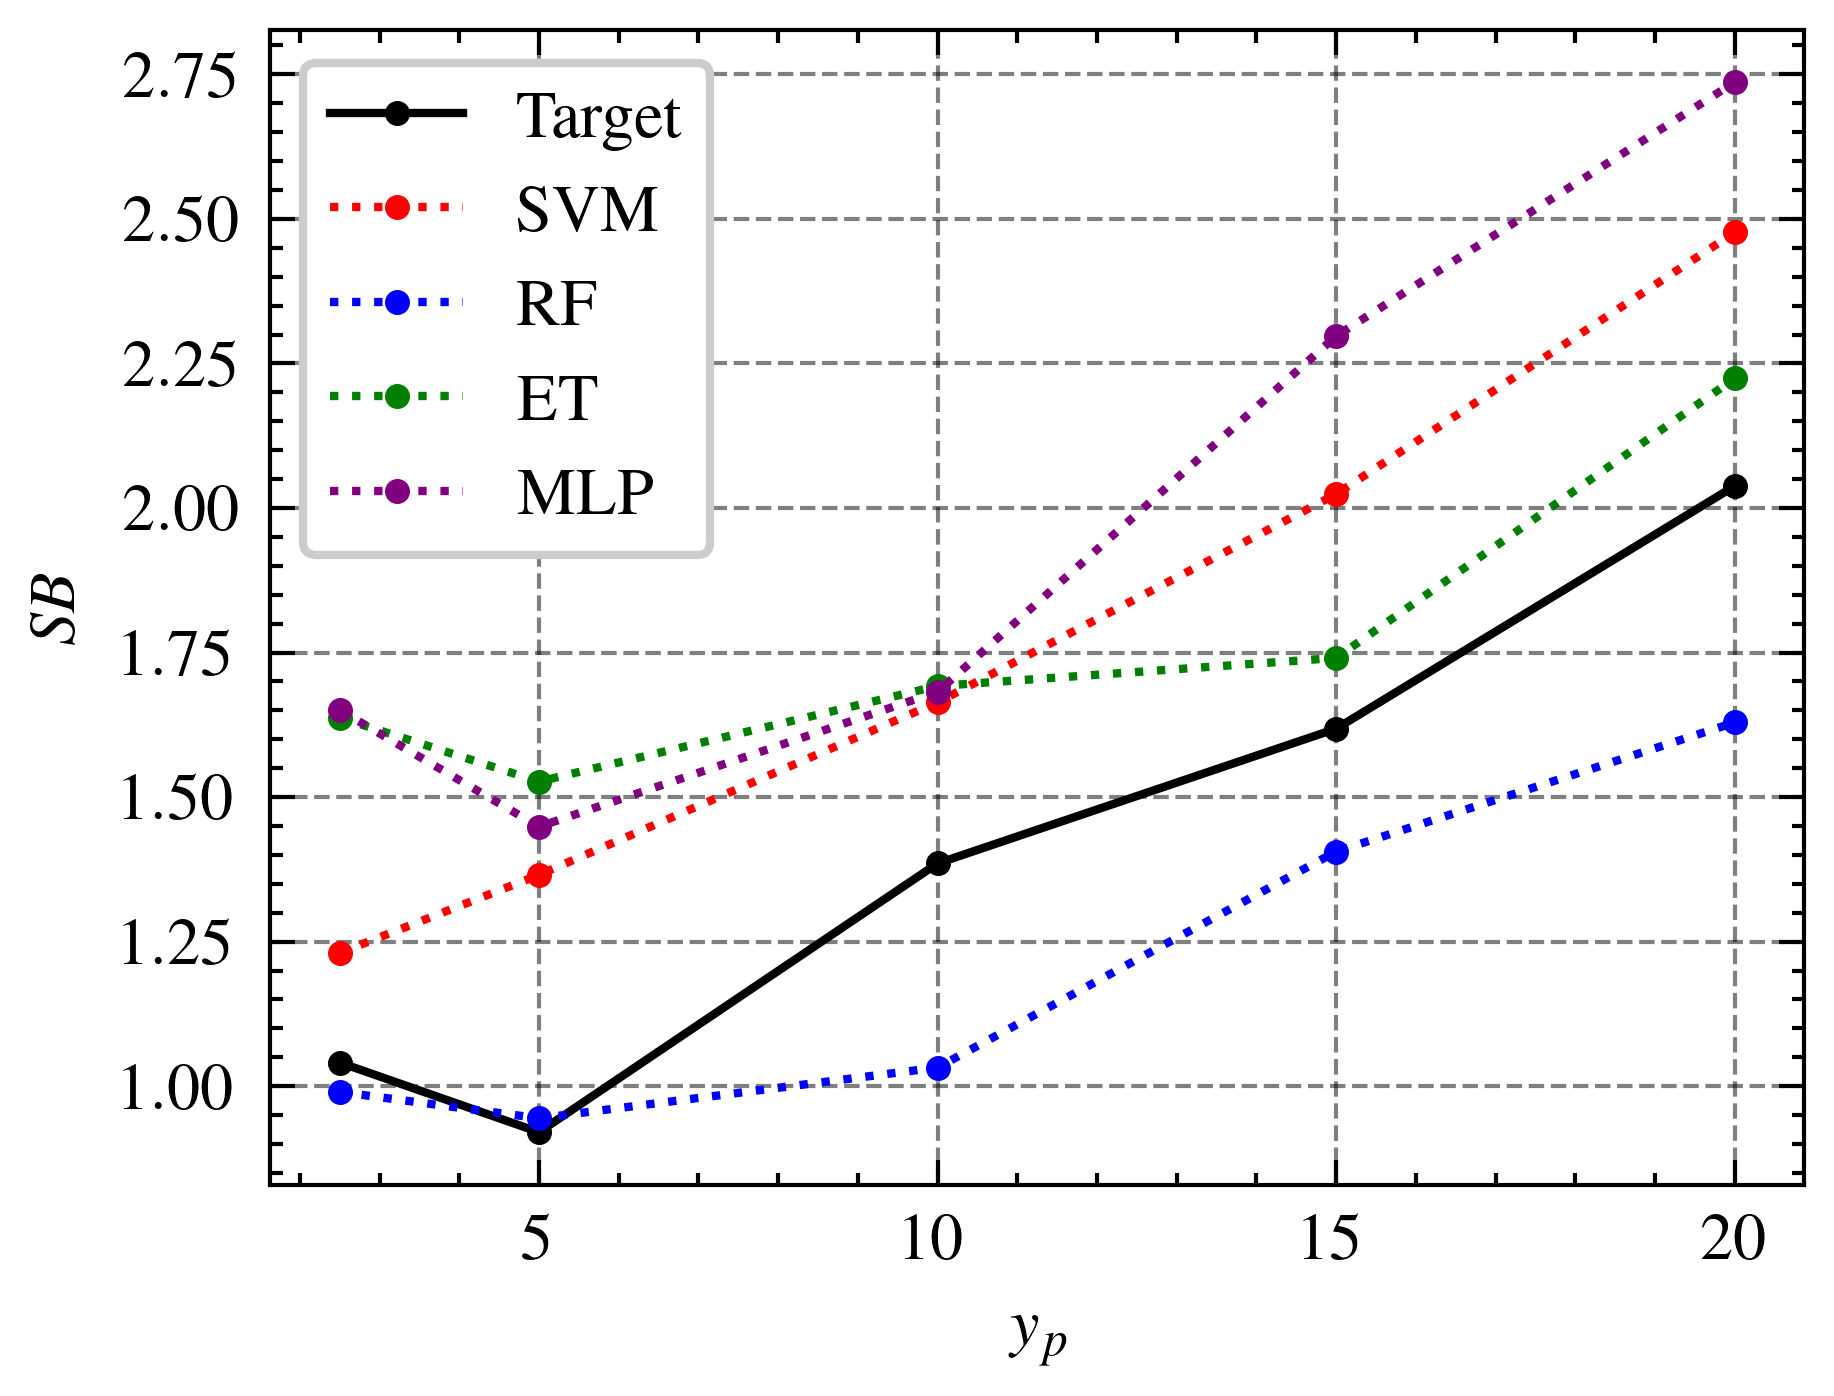
\includegraphics[width=\textwidth]{chap5/images/performance_50_1}
            \caption{V: 50, t: 1}
            \label{fig:performance-50_1}
        \end{subfigure}
    \end{tcolorbox}
    \caption{Performance plots for case C}
    \label{fig:performance-case-c}
\end{figure}

The best overall performing models are the \ac{MLP} and the \ac{SVM} model.
As seen before, the model performs consistent across all thee scenarios, indicating that it can
effectively handle a broad range of V/t ratios also outside the recommended industry guidelines
range.
Therefore the chosen models for more detailed analysis are the \ac{MLP} and the \ac{SVM} model.

Overall it can be said that the models are able to predict the spring back with high accuracy.
For bad predictions the error is less than 0.25 mm, which is within the tolerance of the
most manufacturing processes (This it not true yet).


\subsection*{Global Model-Agnostic Methods}
In the following section global-model-agnostic methods are are applied to the trained machine
learning models in order to understand the overall behavior of the models.

There are two commonly used methods for analyzing the relationship between input features and the
target variable: feature dependence plots and partial dependence plots.
In the case of \ac{MLP} has no built-in feature importance, because the importance of each
feature is determined by the weights assigned to the perceptron.
The \ac{SVM} the feature importance cannot be directly derived from the model beacuse the
algorithms applies a hyperplane that separates the data.
The importance of the feature depeneds on the influence of the hyperplane and that is not easily
measurable.
Therefore not feature importance can be plotted for the two chosen models. Other models like the
random forest have a built-in feature importance, which can be used to analyze the model.

Figure~\ref{fig:feature_impoartances_rf} compares and visualizes the relative
importance of the features used for training the model.
As shown, the thickness is the most important feature followed by distance
and die opening.
The results shows, that all three featured are relevant for the outcome and so no feature can be
removed from the dataset to get a better performance of the model.

\begin{figure}[H]
    \begin{tcolorbox}[arc=0pt,boxrule=0.5pt]
        \centering
        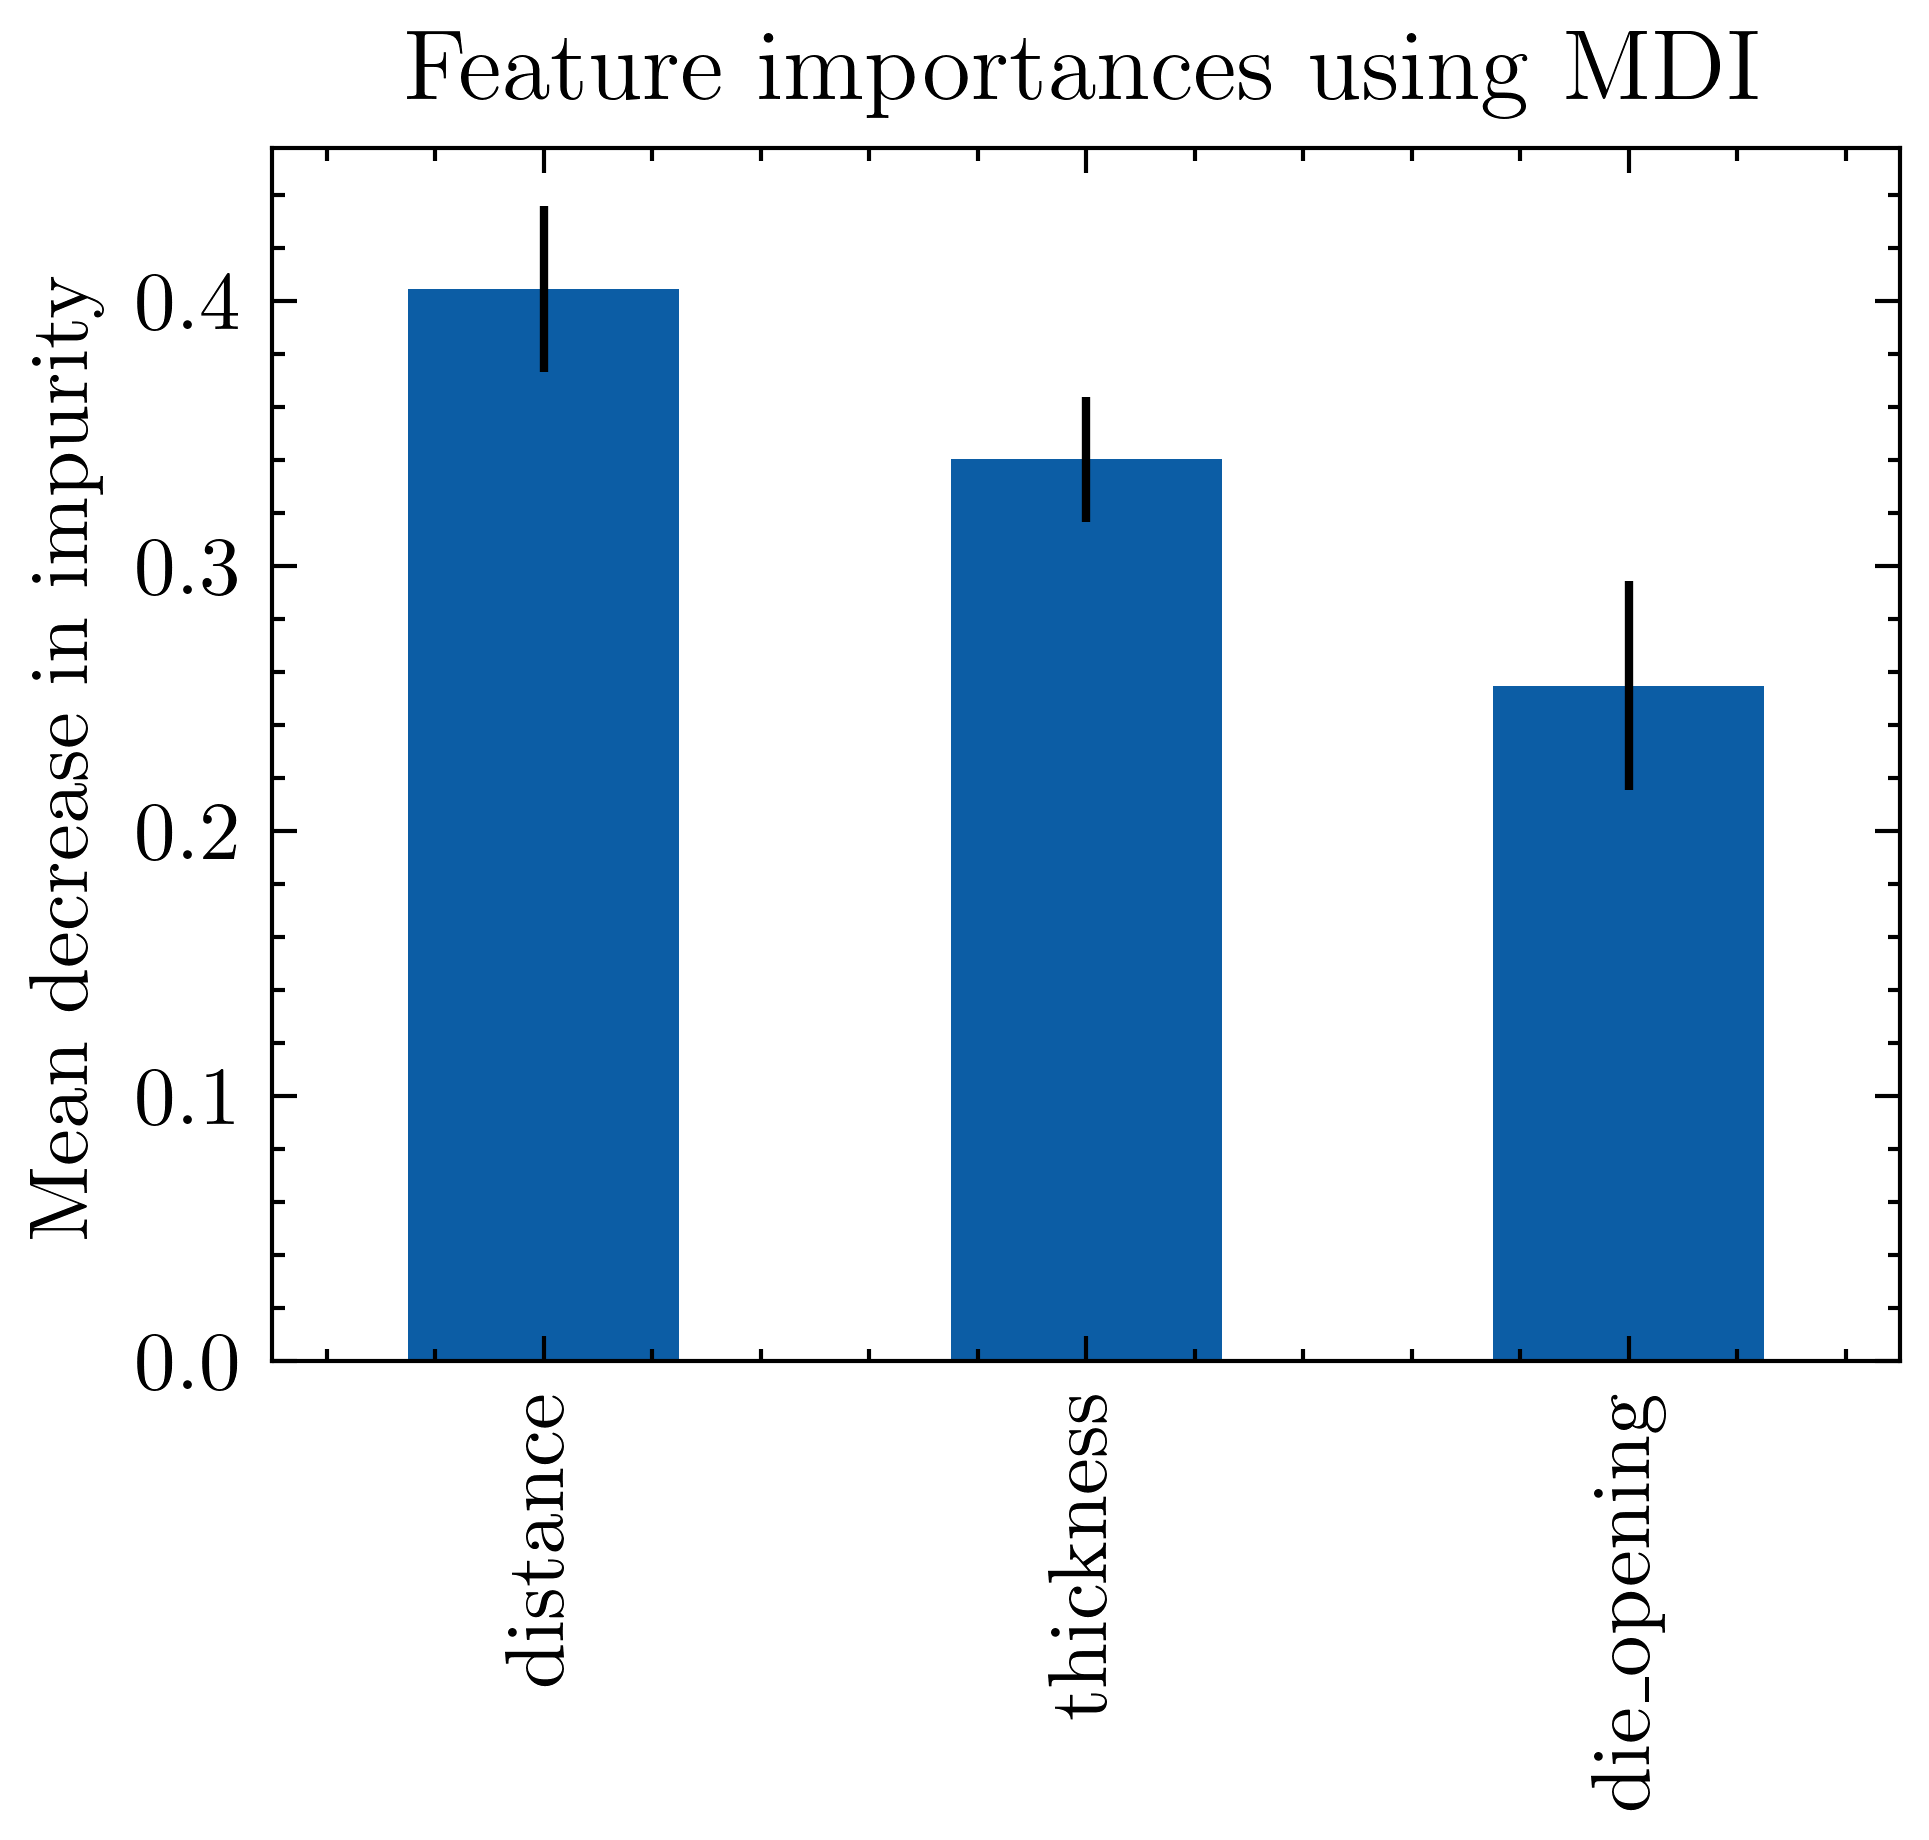
\includegraphics[width=0.9\textwidth]{chap5/images/rf_feature_importances}
    \end{tcolorbox}
    \caption{Feature importance of the random forest model.}
    \label{fig:feature-importances-rf}
\end{figure}

\subsubsection{Partial Dependence}
Feature dependence plots illustrate the relationship between a feature and the target variable.
By analyzing these plots, we can identify which features have the strongest impact on the model's
predictions, making it easier to prioritize and refine our feature selection.

Partial dependence plots, on the other hand, examine the impact of a single input feature on the
target variable while keeping all other features constant.
These plots can help us understand which individual features have the most significant impact on
the target, enabling us to fine-tune our feature engineering and gain deeper insights into the
underlying relationships in our data.

Both of these methods are powerful tools for understanding the role of input features in
predictive modeling, and can be used together to gain a comprehensive understanding of the
factors that drive model performance.

\cite{greenwell2018simple} introduced a another feature importance measure based on partial
dependence.
Partial dependence refers to the relationship between a target variable and a single predictor
variable in a statistical model, while keeping all other predictor variables constant.
A feature that has a consistent partial dependence across all values is less important than a
feature that exhibits significant variations~\cite[p. 117--118]{molnar2020interpretable}.


Figure~\ref{fig:partial_dependence_plots}, we can see the PDPs for two models: Support Vector
Machines (SVM) and Multilayer Perceptron (MLP).
The results show that a higher \(y_p\) value leads to a greater spring back, while increasing the
thickness of the metal sheet results in a lower spring back.
The effect of the die opening is less significant than the other two features, but there is still
a noticeable increase in spring
back with higher die opening.

The PDPs demonstrate that all features exhibit a non-linear relationship with the target variable.
This information can be useful for understanding the behavior of the models and the impact of
different features on the predicted outcome.

\begin{figure}
    \begin{tcolorbox}[arc=0pt,boxrule=0.5pt]
        \centering
        \begin{subfigure}{0.45\textwidth}
            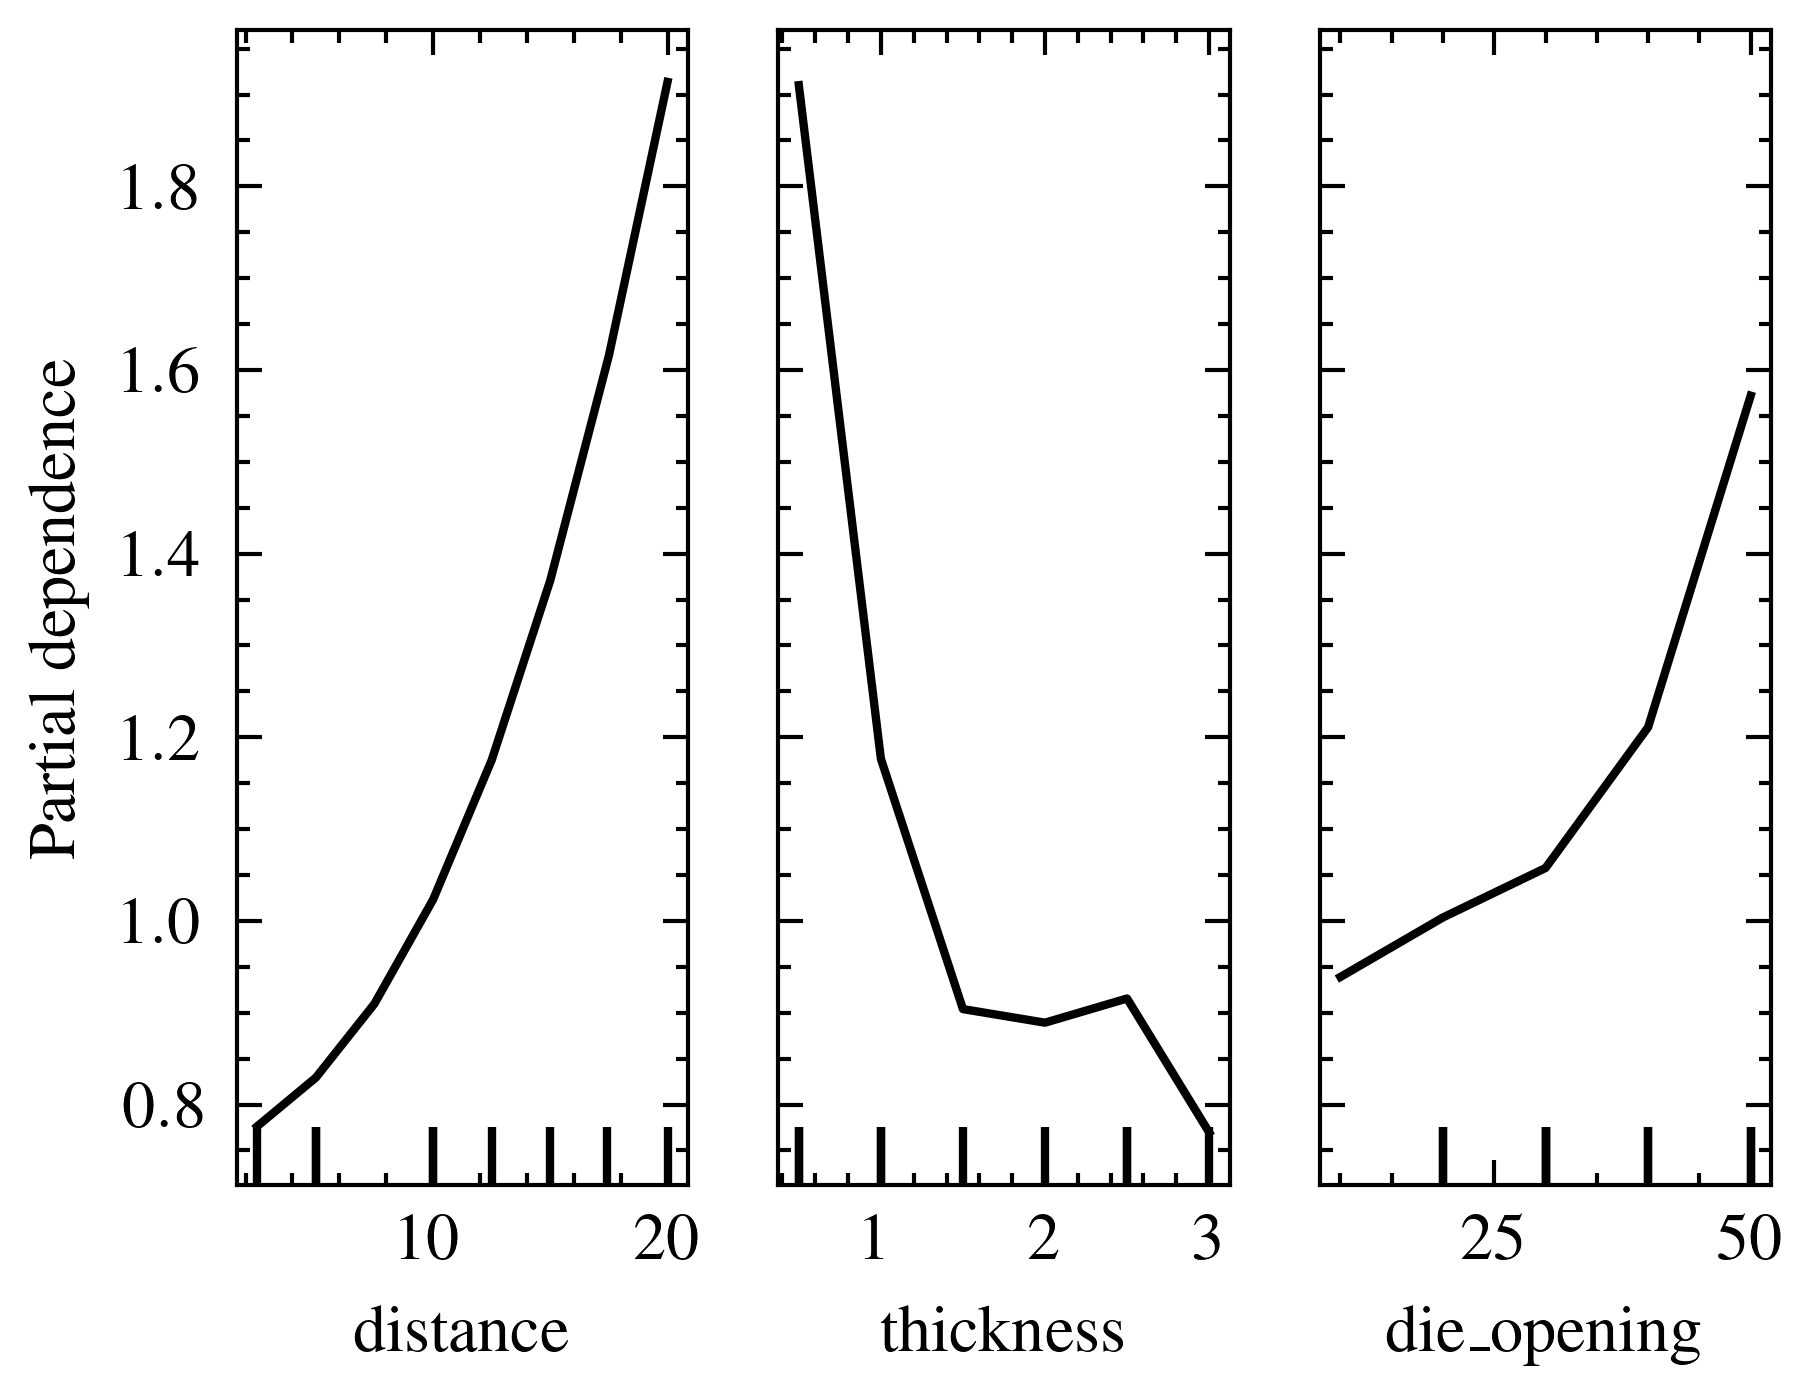
\includegraphics[width=\textwidth]{chap5/images/partial_dependence_SVM}
            \caption{SVM}
            \label{fig:feature_impoartances_rf}
        \end{subfigure}
        \hfill
        \begin{subfigure}{0.45\textwidth}
            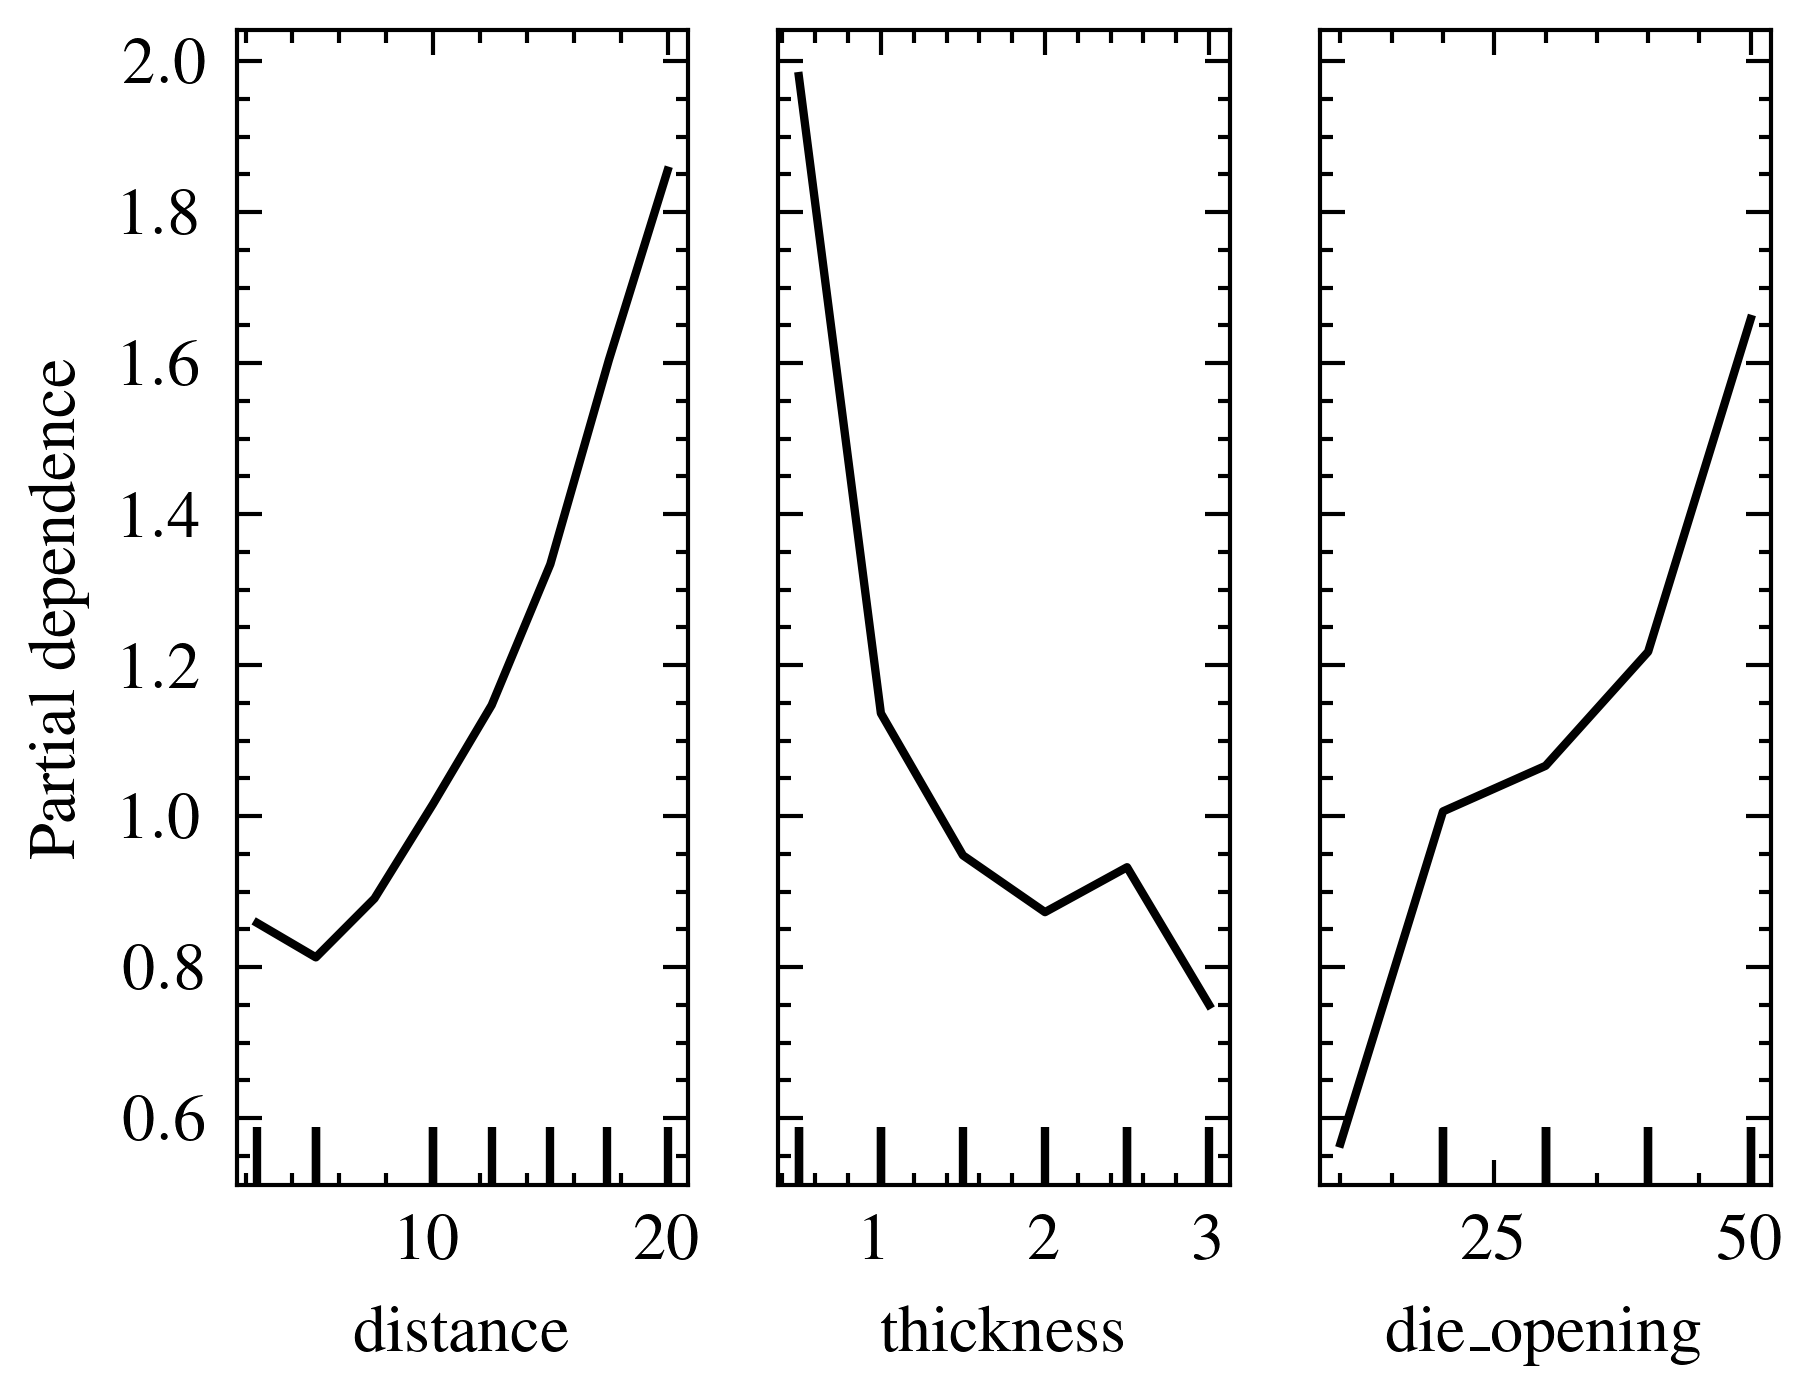
\includegraphics[width=\textwidth]{chap5/images/partial_dependence_MLP}
            \caption{MLP}
            \label{fig:partial_dependence_svm}
        \end{subfigure}
        \hfill
        \caption{Partial dependence plots}

        \label{fig:partial_dependence_plots}
    \end{tcolorbox}
\end{figure}

It is important to note that partial dependence plots and feature importance plots are limited to
identifying linear relationships between features and the target variable.
Since this is not the case as state previously, the results of the partial dependence plots are
alternative models as permutation feature importance and SHAP values are used to gain further
information.

\subsection{Permutation Feature Importance and SHAP}\label{subsec:permutation-feature-importance-
and-shap}

Permutation feature importance's asseses the impact on the model's prediction error when the values
of a feature a randomly permutes. Permutation in this context means the proces of randomly
shuffling the values of a single features while keeping the values of all other feautres unchanged.
Thereby the association between the feature and the actual outcome is disrupted~\cite[p. 157]{
    molnar2020interpretable}.

The importance of a feature is evaluated by assessing the degree to which permuting its values
results in an increase in the prediction error fo the model.
If permuting a features results in a significant increases in errors the features is deemed
important because the model relied on it for making accurate predictions.
Conversely, if permuting a feature doesn't change the prediction error is considered unimportant
because the model didn't utilize it for it's prediction~\cite[p. 158]{molnar2020interpretable}.

Figure~\ref{fig:permutation_feature_importance} shows the permutation feature importance for the
\ac{MLP} and \ac{SVM} models.
Interestingly, the results show that the permutation feature importances for the die opening is
always zero.
This could mean that the die opening is not relevant for the overall decision making of both
models.
The normal feature importance plots showed that die die opening is important so that might not be
explanation.
So most likely the die opening is still and important feature when combined with either the
thickness ore the penetration distance.




\begin{table}[ht]
    \begin{tcolorbox}[arc=0pt,boxrule=0.5pt]
        \centering
        \subfloat[Subtable 1 list of tables text][MLP]{
            \begin{tabular}{lll}
                \toprule
                \multicolumn{3}{}{\textbf{$R^2$}} \\
                \toprule
                thickness   & 1.337 & +/-  0.173542 \\
                \hdashline
                distance    & 1.293 & +/-  0.145488 \\
                \hdashline
                die opening & 0.000 & +/-  0.000000 \\
                \toprule
                \multicolumn{3}{l}{\textbf{$MSE$}} \\
                \toprule
                thickness   & 0.274 & +/-  0.035613 \\
                \hdashline
                distance    & 0.265 & +/-  0.029856 \\
                \hdashline
                die opening & 0.000 & +/-  0.000000 \\
                \bottomline
            \end{tabular}}
        \qquad
        \subfloat[Subtable 2 list of tables text][SVM]{
            \begin{tabular}{lll}
                \toprule
                \multicolumn{3}{}{\textbf{$R^2$}} \\
                \toprule
                distance    & 1.237 & +/-  0.139285 \\
                \hdashline
                thickness   & 1.178 & +/-  0.157247 \\
                \hdashline
                die opening & 0.000 & +/-  0.000000 \\
                \toprule
                \multicolumn{3}{l}{\textbf{$MSE$}} \\
                \toprule
                distance    & 0.254 & +/-  0.028583 \\
                \hdashline
                thickness   & 0.242 & +/-  0.032269 \\
                \hdashline
                die opening & 0.000 & +/-  0.000000 \\
                \bottomline
            \end{tabular}}
    \end{tcolorbox}
    \caption{Permutation feature importance}
    \label{tab:permutation_feature_importance}
\end{table}

To investigate the joint performance of the die opening feature with the other two features,
again partial dependence plots can be used.
Figure~\ref{fig:partial_dependence_plots} shows a two-way partial dependence plot for the
\ac{MLP} model.
The x- and y-axes represent the thickness and the distance, respectively.
The slope of the contour lines indicates the direction of the effect of the die opening on the
prediction.
The contour lines are colored and labeled according to the value of the prediction.
It can be seen that the contour lines are not parallel which suggest the two features are
interaction with each other and therefore have a joint effect on the model prediction.

Therefore it can be concluded than different to the first appearance in the partial dependence
plots the die opening is not irrelevant for the model prediction.

\begin{figure}[H]
    \begin{tcolorbox}[arc=0pt,boxrule=0.5pt]
        \centering
        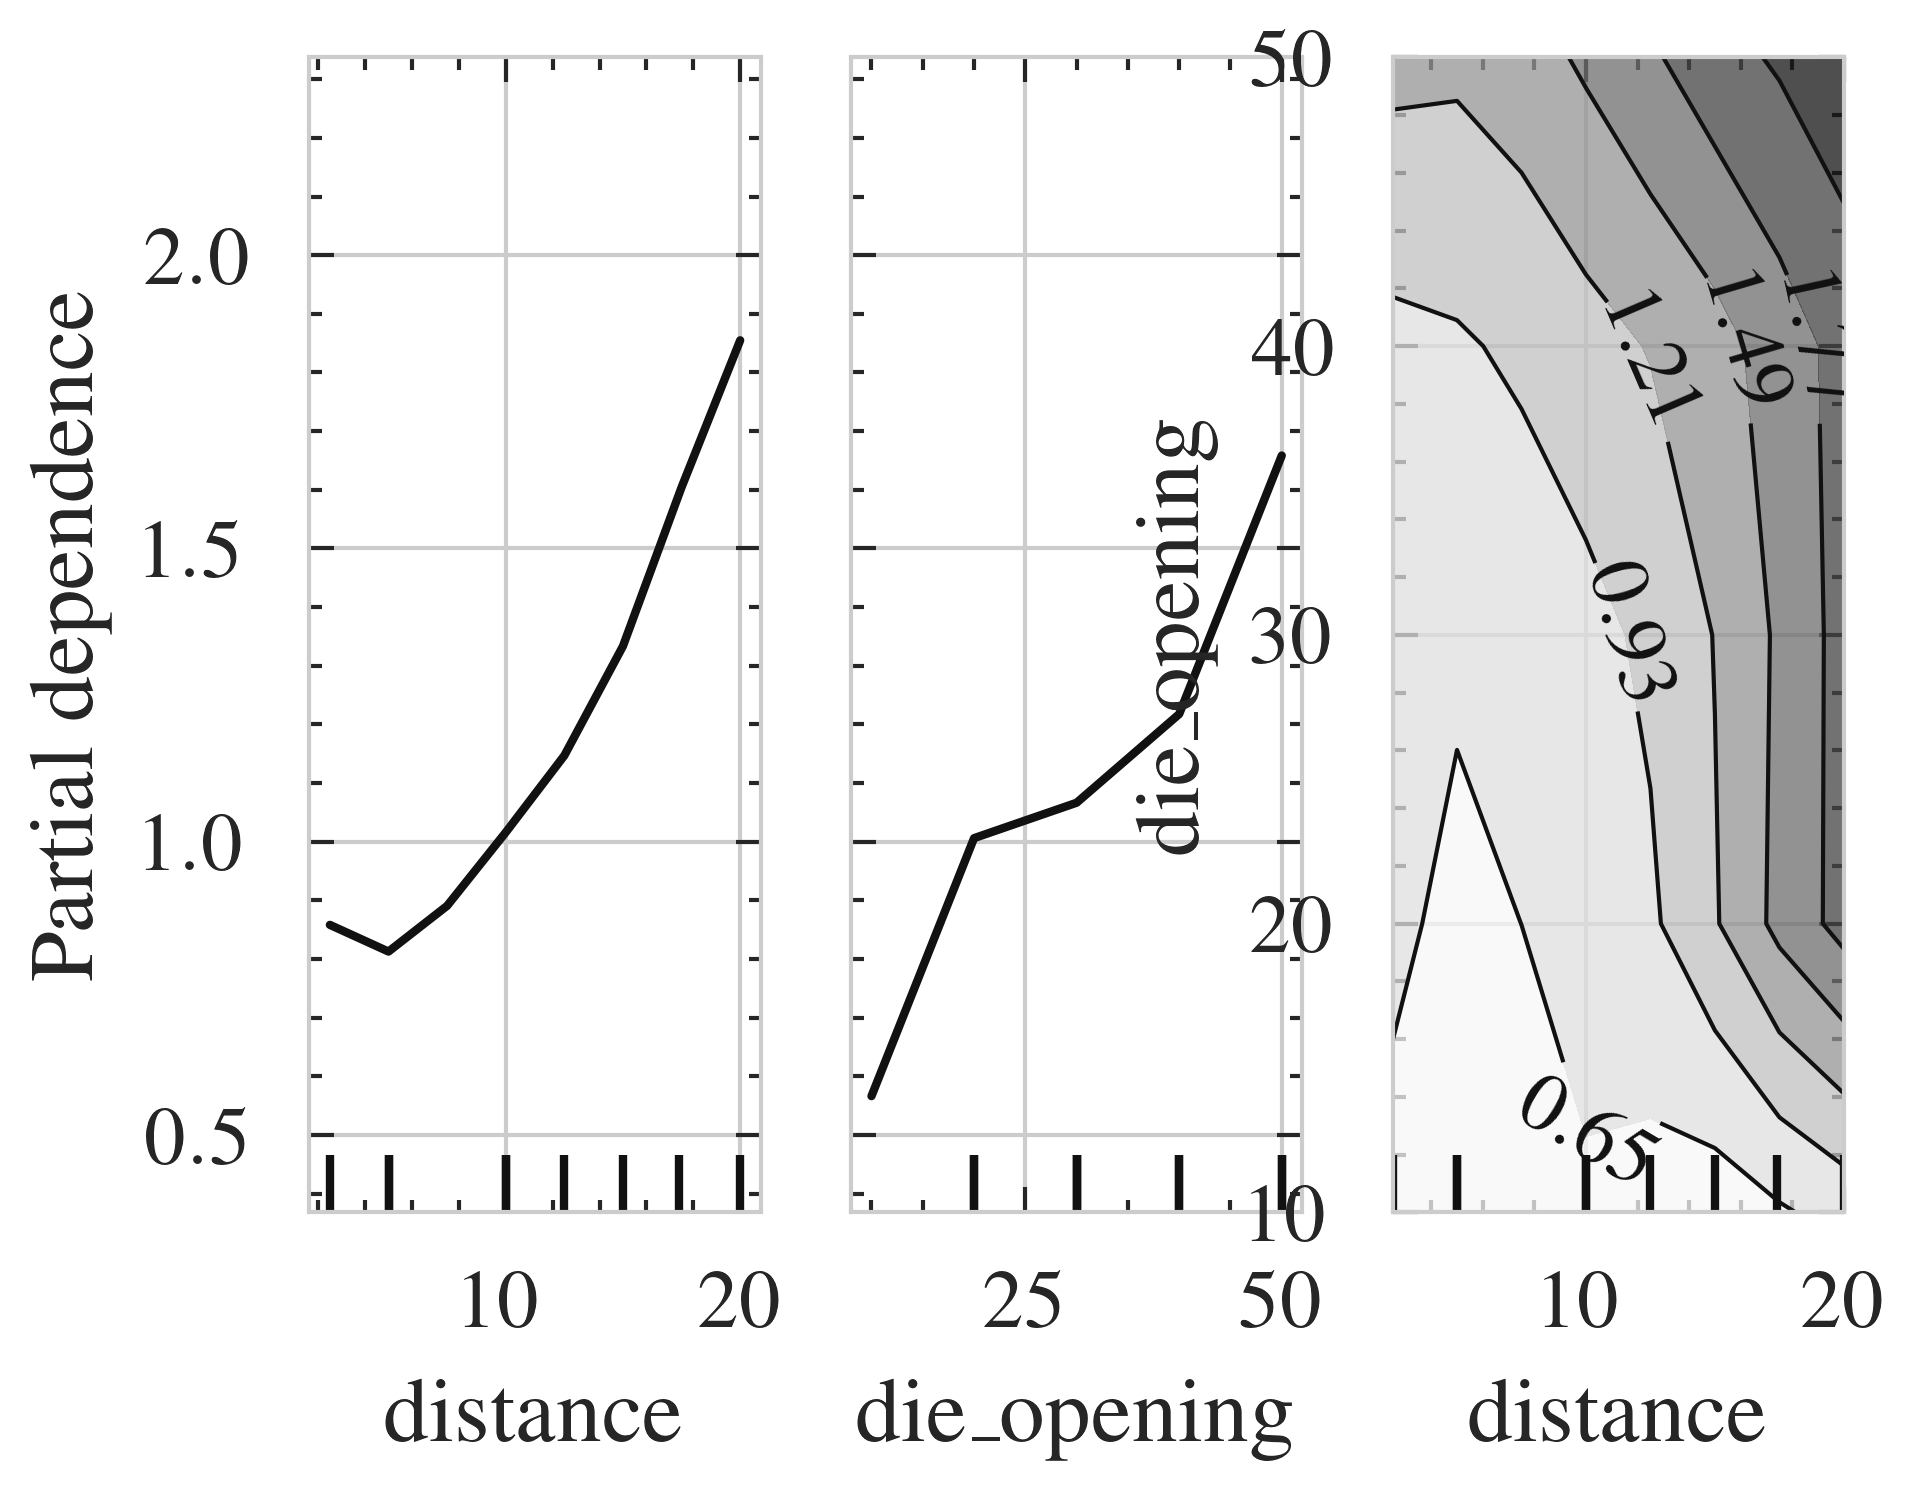
\includegraphics[width=0.9\textwidth]{chap5/images/pdp_distance_die_opening}
    \end{tcolorbox}
    \caption{DPD distance and die opening}
    \label{fig:dpd-distance-die-opening}
\end{figure}

\subsection*{Local Model Agnostic Methods}
Local interpretability refers to the ability to understand the behavior of the model for a
specific instance and is often used to explain the predictions of a model.
Model agnostic methods can be used to explain the predictions of any model type~\cite{
    molnar2020interpretable}.

Local methods rely on interpreting individual instances from a dataset, and as such, it is
crucial to select representative samples.
One way to achieve this is by considering the V/t ratio of each instance.

\subsection{LIME}\label{subsec:lime}
The LIME method stands for Local interpretable model-agnostic explanations
and a model itself that can be used to explain the predictions of any machine
learning model, the model is treated as a black-box~\cite{ribeiro2016model}.
To accomplish this, LIME generates a new dataset with permuted samples along with the predictions
made by the black box model for each sample.
Using this dataset, LIME trains an interpretable model that is given weights based on the
proximity of the sampled instance to the instance of interest.
The interpretable model can be any model that is considered interpretable, such as a Liner
Regression or Decision Trees.

This approach allows LIME to provide explanations for individual predictions by approximating the
behavior of the black box model in a localized and interpretable way~\cite[p. 185]{
    molnar2020interpretable}.

\cite{molnar2020interpretable} express local surrogate models like LIME as follows:

\begin{tcolorbox}[arc=0pt,boxrule=0.5pt]
    \begin{equation}
        explanation(x) = arg\; min\underset{g \in G}\; L(f,g,\pi_x) + \Omega(g)
    \end{equation}
\end{tcolorbox}

The model for explaining a certain instance $x$ is represented by the model $g$ (such as a
linear regression model), which reduces the loss (for example \ac{MSE}), measuring how closely
the explanation aligns with the prediction made by the original model $f$ (for instance, an
\ac{MLP} model).
At the same time, the model complexity $\Omega(g)$ should remain low.
The set of all possible linear regression models is referred to as $G$ , which encompasses all
potential explanations.
The proximity measure, denoted as $\pi_x$ , determines the size of the area surrounding the area
surrounding the instance $x$ that is taken into account for the
explanation~\cite[p. 185]{molnar2020interpretable}.

LIME mainly provides instance explanations in the form of feature importance values.
It can show the predicted values along with the explanations on how which features contributed
in which direction to the prediction.
This can be seen similar to PDP plots but instead of showing the average effect of a feature
on the the overall prediction of the model, it shows the effect of a feature on the prediction
for a specific instance.
One instance in this case consists of the thickness, distance die opening and the corresponding
spring back value.


\textit{If I have questions for specific instances I should put them here.}



    \chapter{Conclusions}

\section{Revisiting the Aims and Objectives}

\section{Critique and Limitations}

\section{Future Work}

\section{Final Remarks}

%    \input{chap_test/test}
    \appendix
    \chapter{Appendix}\label{ch:appendix}

\section*{Machine Configuration}\label{sec:machine-configuration}

\begin{table}[H]
    \begin{tcolorbox}[arc=0pt,boxrule=0.5pt]
% \sisetup{group-minimum-digits = 4}
        \centering
        \begin{tabular}{ll}
            \toprule
            \textbf{Parameter} & \textbf{Value}
            \\
            \toprule
            andere Geschwindigkeit für Entlastung & 300 mm/min           \\
            Anzahl Stufen                         & 4                    \\
            Anzahl Zyklen                         & 1                    \\
            Automatische Kraftnullung             & Nein                 \\
            Geschwindigkeit Vorlaufwe             & 100 mm/min           \\
            Geschwindigkeit Zyklus                & 80 mm/min            \\
            Keilspannfaktor                       & 5 bar/kN             \\
            LE-Geschwindigkeit                    & 100 mm/min           \\
            \hdashline
            Maschinendaten                        & 1454MO WN:805754     \\
            Traversenwegaufnehmer                 & WN:805754            \\
            Kraftsensor                           & ID:0 WN:820243 20 kN \\
            \hdashline
            Material                              & Stahl                \\
            Prüfart                               & Druck                \\
            Prüfgeschwindigkeit                   & 5 mm/min             \\
            Prüfnorm                              & DIN 178              \\
            Vorkraft                              & 1 N                  \\
            Vorkraft-Geschwindigkeit              & 100mm/min            \\
            \bottomrule
        \end{tabular}
    \end{tcolorbox}
    \caption{Overview of the used machine learning models and their metrics.}
    \label{tab:machine-config}
\end{table}


\section*{Technology Tables}\label{sec:technology-tables}

\begin{figure}[h]
    \begin{tcolorbox}[arc=0pt,boxrule=0.5pt]
        \centering
        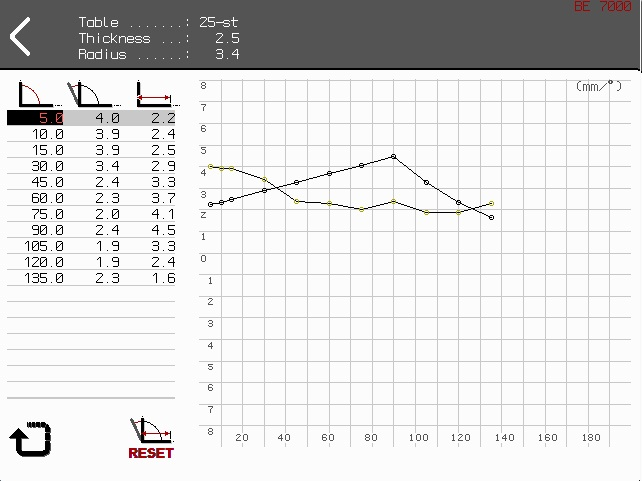
\includegraphics[width=1\textwidth,
            clip]{schwenkbiegen_1}
    \end{tcolorbox}
    \caption{Example of an technology table.}
    \label{fig:technology-table}
\end{figure}

\section*{Hyper Parameters}\label{sec:hyper-parameters}

\subsection*{Decision Tree}
Grid search cross validation was used to find the best hyper-parameters for
the decision tree.
All hyper-parameters are summarized in Table~\ref{tab:hyperparameters_decision_tree}.

\begin{table}[H]
    \begin{tcolorbox}[arc=0pt,boxrule=0.5pt]
        \sisetup{group-minimum-digits = 4}
        \centering
        \begin{tabular}{ll}
            \toprule
            \thead{\textbf{Hyperparameter}} & \thead{\textbf{Value}} &
            \thead{\textbf{Description}}
            \\
            \toprule
            criterion & absolute\_error
            \hdashline
            max\_depth & 30 \\
            \hdashline
            min\_samples\_split & 4 \\
            \hdashline
            min\_weight\_fraction\_leaf & 0. \\
            \hdashline
            splitter & random \\
            \hdashline
            ccp_alpha & 0.0 \\
            \bottomrule
        \end{tabular}
        \caption{Hyperparameters of \ac{DT} model.}
        \label{tab:hyperparameters_decision_tree}
    \end{tcolorbox}
\end{table}

\subsection*{Random Forest}

\begin{table}[h]
    \begin{tcolorbox}[arc=0pt,boxrule=0.5pt]
        \sisetup{group-minimum-digits = 4}
        \centering
        \begin{tabular}{ll}
            \toprule
            \thead{\textbf{Hyperparameter}} & \thead{\textbf{Value}} &
            \thead{\textbf{Description}}
            \\
            %  \unit{(Kcal\per\mole)\squared}}} & \thead{RMSD l.b.} &
            %  \thead{RMSD u.b.}  \\
            \toprule
            n\_estimators & 10 & The number of trees in the forest.
            \\
            \hdashline
            criterion & absolute\_error \\
            \hdashline
            max\_depth & 30 \\
            \hdashline
            min\_samples\_split & 4 \\
            \hdashline
            min\_samples\_leaf & 2 \\
            \hdashline
            max\_features & auto \\
            \hdashline
            max\_leaf\_nodes & X \\
            \hdashline
            max\_leaf\_nodes & X \\
            \bottomrule
        \end{tabular}
        \caption{Hyperparameters of the \ac{RF} model.}
        \label{tab:hyperparameters_rf}
    \end{tcolorbox}
\end{table}

\subsection*{Extra Trees}

\begin{table}[h]
    \begin{tcolorbox}[arc=0pt,boxrule=0.5pt]
        \sisetup{group-minimum-digits = 4}
        \centering
        \begin{tabular}{ll}
            \toprule
            \thead{\textbf{Hyperparameter}} & \thead{\textbf{Value}} &
            \thead{\textbf{Description}}
            \\
            %  \unit{(Kcal\per\mole)\squared}}} & \thead{RMSD l.b.} &
            %  \thead{RMSD u.b.}  \\
            \toprule
            bootstrap & True
            \\
            \hdashline
            criterion & absolute\_error \\
            \hdashline
            max\_depth & 6 \\
            \hdashline
            min\_samples\_split & 4 \\
            \hdashline
            min\_samples\_leaf & 1 \\
            \bottomrule
        \end{tabular}
        \caption{Hyperparameters of the Extra Trees model.}
        \label{tab:hyperparameters_et}
    \end{tcolorbox}
\end{table}

\subsection*{Gradient Boosting}

\begin{table}[h]
    \begin{tcolorbox}[arc=0pt,boxrule=0.5pt]
        \sisetup{group-minimum-digits = 4}
        \centering
        \begin{tabular}{ll}
            \toprule
            \thead{\textbf{Hyperparameter}} & \thead{\textbf{Value}} &
            \thead{\textbf{Description}}
            \\
            \toprule
            loss & huber
            \\
            \hdashline
            learning\_reate & 0.1 \\
            \hdashline
            max\_depth & 4 \\
            \hdashline
            min\_samples\_split & 3 \\
            \hdashline
            min\_samples\_leaf & 3 \\
            \hdashline
            n\_estimators & 200 \\
            \bottomrule
        \end{tabular}
        \caption{Hyperparameters of the Extra Trees model.}
        \label{tab:hyperparameters_gradient_boosting}
    \end{tcolorbox}
\end{table}

\subsection{Extra Trees}\label{subsec:extra-trees}

\begin{table}[h]
    \begin{tcolorbox}[arc=0pt,boxrule=0.5pt]
        \sisetup{group-minimum-digits = 4}
        \centering
        \begin{tabular}{lll}
            \toprule
            \thead{\textbf{Hyperparameter}} & \thead{\textbf{Value}} &
            \thead{\textbf{Description}}
            \\
            \toprule
            bootstrap & True \\
            \\
            \hdashline
            learning\_reate & 0.1 \\
            \hdashline
            criterion & 'absolute_error' \\
            \hdashline
            max\_depth & 6 \\
            \hdashline
            min\_samples_split & 4 \\
            \hdashline
            n\_estimators & 10 \\
            \hdashline
            min\_samples\_leaf & 1 \\
            \bottomrule
        \end{tabular}
        \caption{Hyperparameters of the Extra Trees model.}
        \label{tab:hyperparameters_gradient_boosting}
    \end{tcolorbox}
\end{table}


\subsection*{SVM}

\begin{table}[h]
    \begin{tcolorbox}[arc=0pt,boxrule=0.5pt]
        \sisetup{group-minimum-digits = 4}
        \centering
        \begin{tabular}{ll}
            \toprule
            \thead{\textbf{Hyperparameter}} & \thead{\textbf{Value}} &
            \thead{\textbf{Description}}
            \\
            \toprule
            bootstrap & True \\
            \hdashline
            criterion & absolute\_error \\
            \hdashline
            min\_samples\_split & 4 \\
            \hdashline
            max\_depth & 6 \\
            \hdashline
            min\_samples\_leaf & 1 \\
            \hdashline
            n\_estimators & 10 \\
            \bottomrule
        \end{tabular}
        \caption{Hyper-paramters of the SVM model.}
        \label{tab:hyperparameters_svm}
    \end{tcolorbox}
\end{table}

\subsection*{MLP}

\begin{table}[H]
    \begin{tcolorbox}[arc=0pt,boxrule=0.5pt]
        \sisetup{group-minimum-digits = 4}
        \centering
        \begin{tabular}{ll}
            \toprule
            \thead{\textbf{Hyperparameter}} & \thead{\textbf{Value}} &
            \thead{\textbf{Description}}
            \\
            %  \unit{(Kcal\per\mole)\squared}}} & \thead{RMSD l.b.} &
            %  \thead{RMSD u.b.}  \\
            \toprule
            random\_state & 1 \\
            \hdashline
            solver & lbfgs \\
            \hdashline
            max\_iter & 5000 \\
            \hdashline
            alpha & 0.01 \\
            \hdashline
            hidden\_layer\_sizes & (100, 100) \\
            \hdashline
            learning\_rate & constant \\
            \bottomrule
        \end{tabular}
        \caption{Hyperparameters of the \ac{MLP} model.}
        \label{tab:hyperparameters_mlp}
    \end{tcolorbox}
\end{table}











    \pagestyle{umpageback}
    {\backmatter
    % Bibliography
    \if@openright\cleardoublepage\else\clearpage\fi

    \bibliographystyle{apa} %% specific plainnat does not show url for articles
    % Use something like https://flamingtempura.github.io/bibtex-tidy/ to clean all your bibtex
    % entries
    {    \scriptsize\bibliography{
        chap1/introduction_biblio,
        chap2/background_and_lit_overview_biblio,
        chap2/theoretical_foundations_biblio,
        chap3/research_methodology_biblio,
        chap4/build_biblio,
        chap5/evaluate_biblio,
    }}
    \printindex
    }

\end{document}

%%% The End %%%
